\chapter{Hadronic recoil calibration}\label{sec:HadrCalib}
\minitoc

As mentioned in Sec.~\ref{sec:EtMissRec} due to discrepancies between the data and simulation, this analysis uses a hadronic recoil algorithm for the missing transverse energy reconstruction. The missing transverse energy significantly affects the W-boson measurement, so it is important to have a solid understanding  of discrepancies in hadronic recoil.
In Sec.~\ref{sec:HRIntro} the hadronic recoil calibration procedure is described. Sec.~\ref{sec:HRReso} presents the procedure of the hadronic recoil resolution correction. In Sec.~\ref{sec:HRBias} the hadronic recoil bias determination is presented. The summary of the hadronic recoil calibration studies is given in Sec.~\ref{sec:HRSum}. 

\section{Introduction}\label{sec:HRIntro}

\begin{figure}[!bp]
\centering
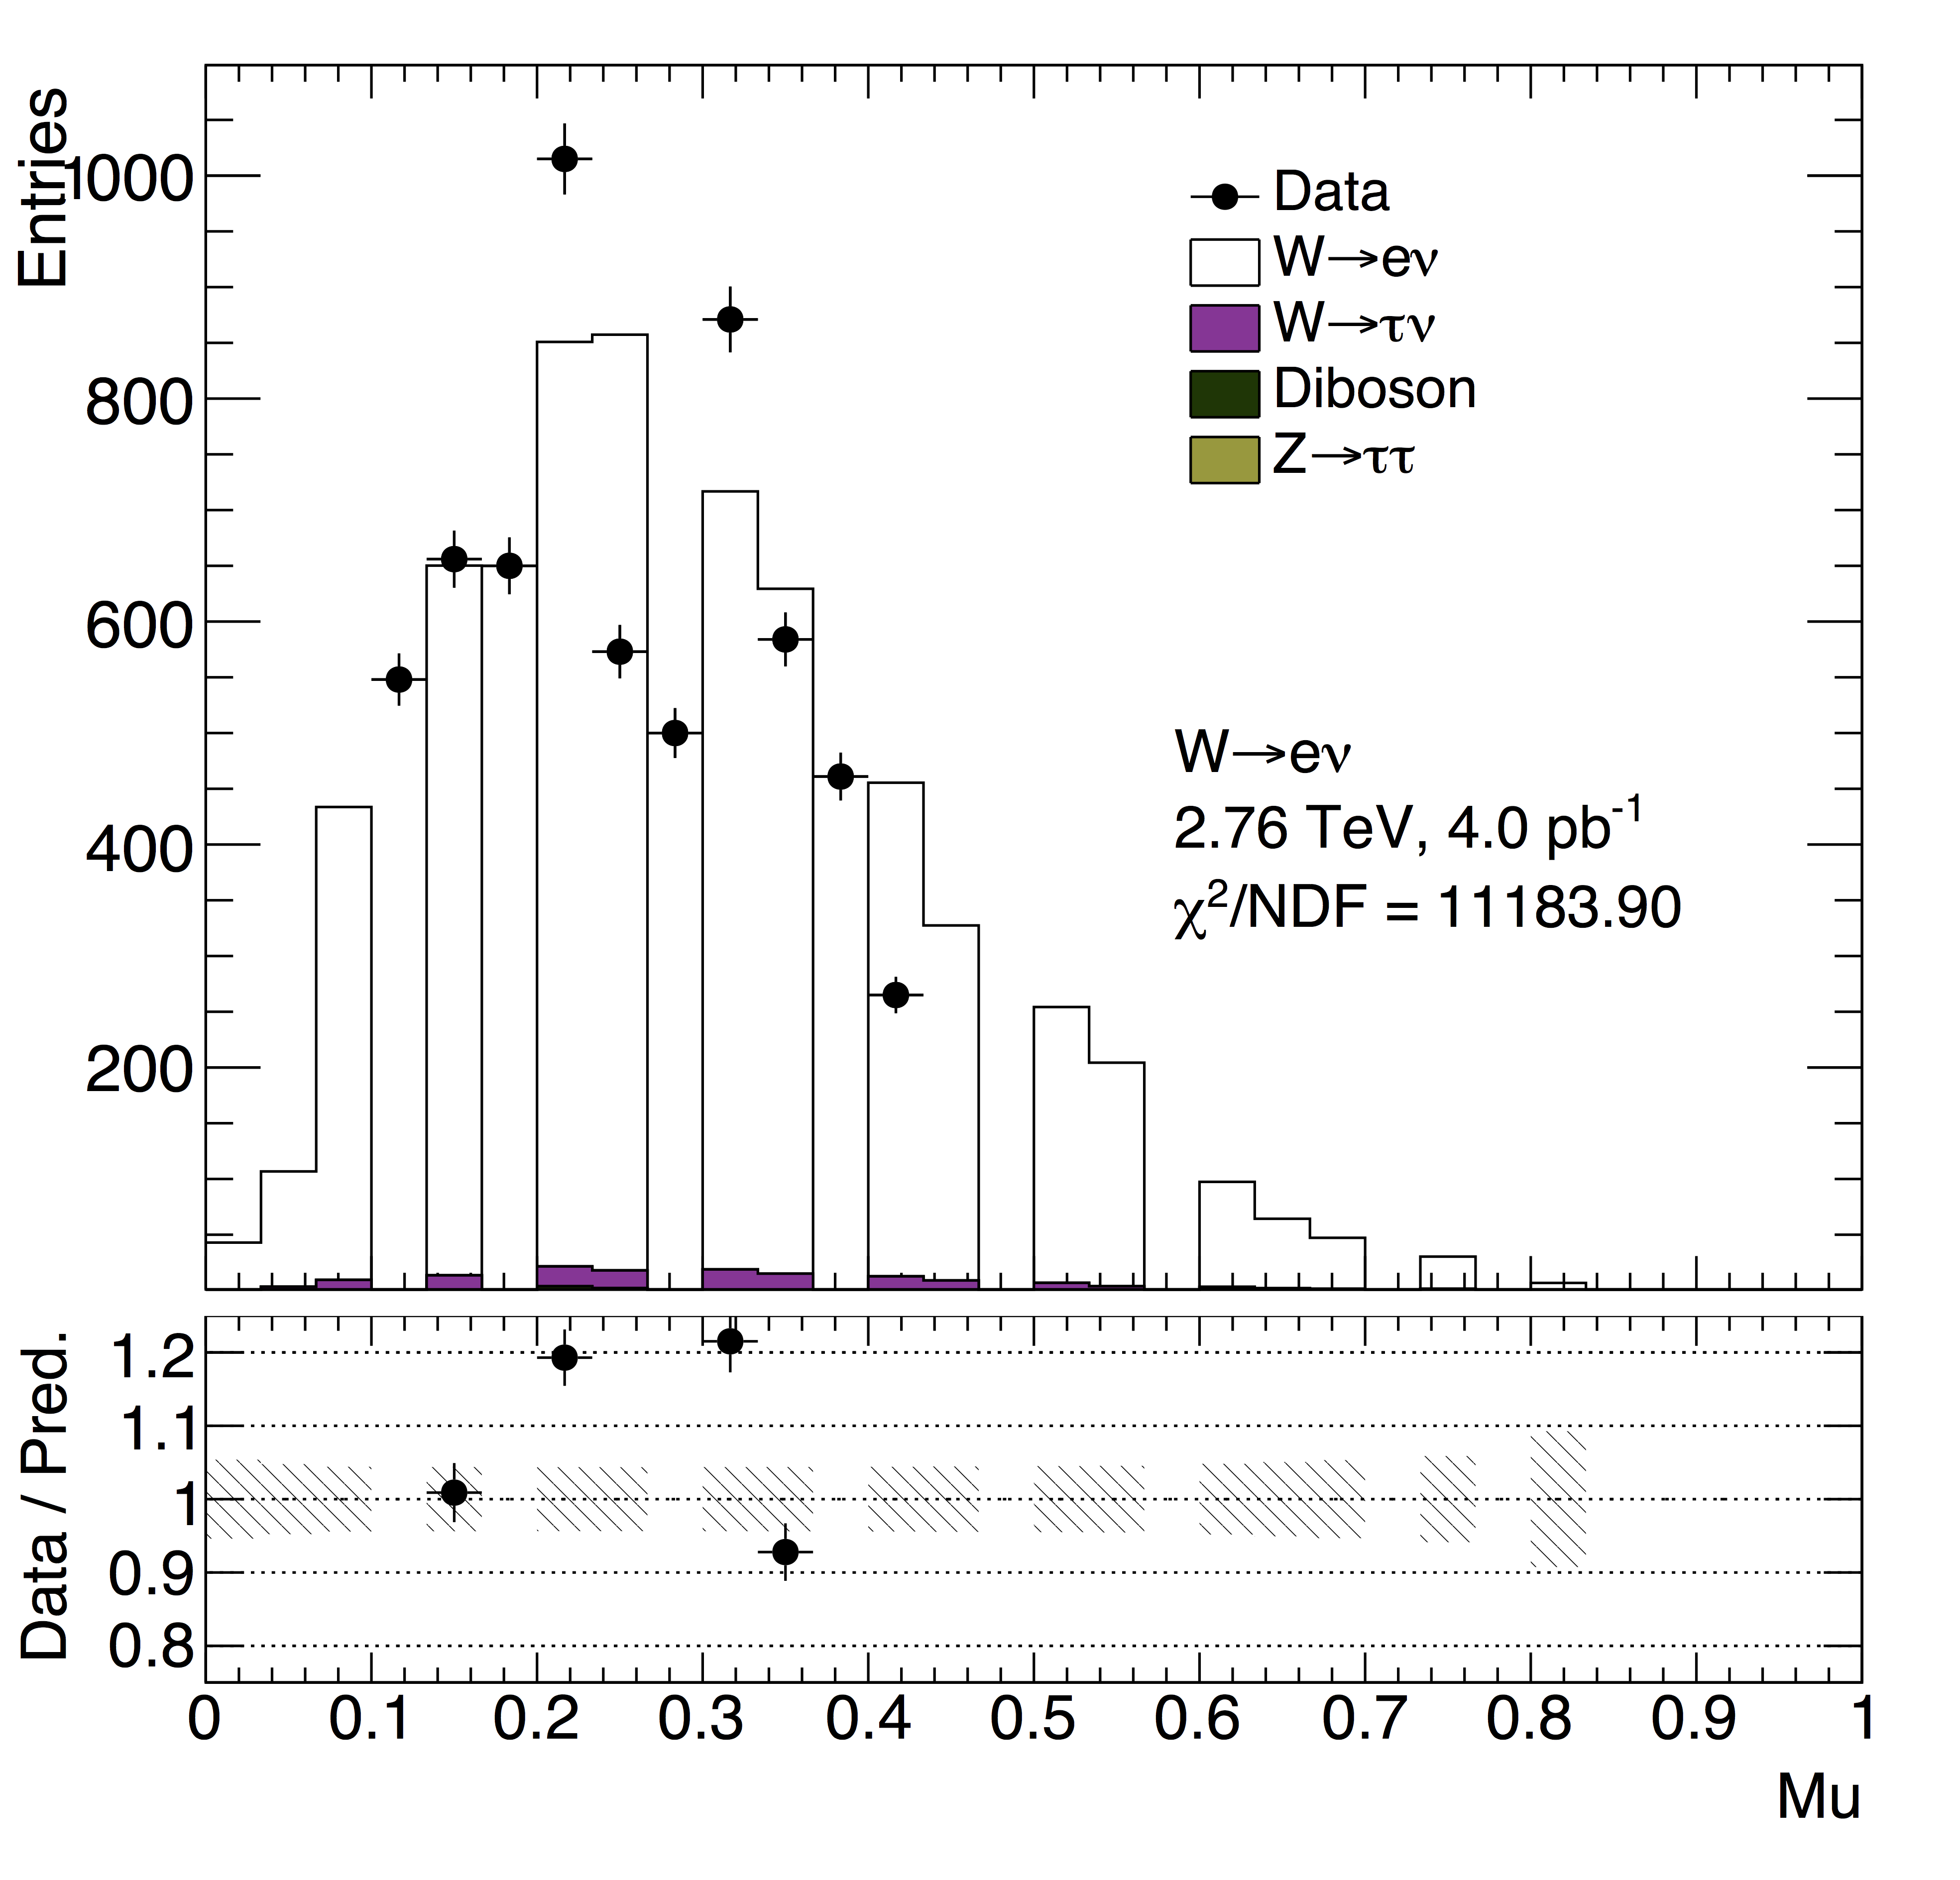
\includegraphics[width=0.5\textwidth]{HadronRecoil/W_Event_Mu.png}
\caption{Mean number of interactions per bunch crossing in \wenu analysis.}
\label{HadrRecoil:mu}
\end{figure} 

This analysis uses a standard hadronic recoil calibration procedure, described in details in \cite{HRCorrections}, that was modified and adapted for the $\sqrt{s}$ = 2.76 TeV data sample.  The procedure, described in \cite{HRCorrections} consists of three main steps. 

In the first step, the differences in the pile-up modeling are corrected. Possible discrepancies are usually corrected by reweighting an average number of interactions per bunch crossing in MC to match the data.  Due to the precision of the pile-up modeling at $\sqrt{s}$ = 2.76 TeV (Fig.~\ref{HadrRecoil:mu}) the precise reweighting is impossible. However, since the mean number of interactions per bunch crossing is below 1, the effect of pile-up mismodelling  on \etmiss distribution can be neglected.

In the second and the third steps, possible discrepancies in the resolution and the scale of the hadronic recoil are corrected. The performance of hadronic recoil algorithm can be studied in MC simulation using the projection of hadronic recoil vector $\vec{HR}$ on the direction of the transverse momentum of the vector boson, as shown in Fig.~\ref{ris:HadrRecoilTruthPt}. This projection can be divided into perpendicular \uperp and parallel \upar components as follows:
\begin{equation}
\upar=\vec{v_{xy}}\cdot\vec{HR},
\end{equation}
\begin{equation}
\uperp=v_x\cdot HR_y - v_y \cdot HR_x,
\end{equation}
where $\vec{v_{xy}}$ is a unit vector along the transverse component of a vector boson momentum and $v_x$ and $v_y$ are its projections on the $x$ and $y$ axis respectively. In the case of the true kinematics $\upar=-P_T^{bos}$ and $\uperp = 0$. However, the limited calorimeter resolution is causing relatively wide distributions for these projections. The parallel component \upar is sensitive to a possible bias in the hadronic recoil, while the perpendicular \uperp can be used for determination of the resolution discrepancies. The mean and the width of these distributions can depend on different variables, such as a mean number of interactions in an event per bunch crossing, hadronic activity and $P_{T}^{bos}$. 


\begin{figure}[!tbp]
\begin{center}
\begin{minipage}[h]{0.49\linewidth}
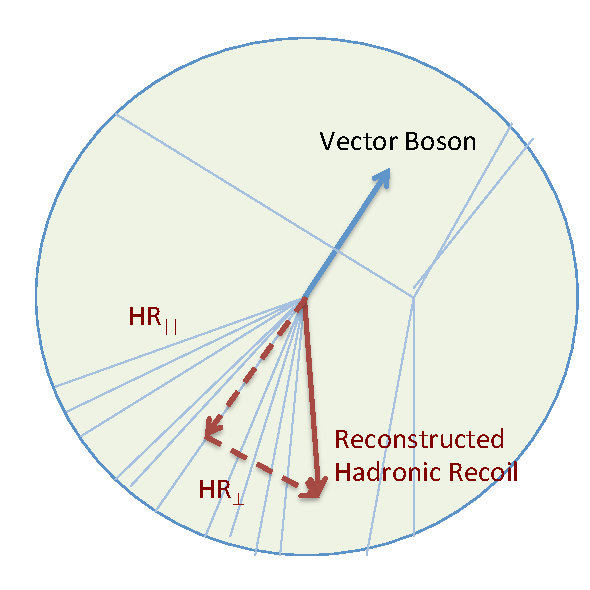
\includegraphics[width=1\textwidth]{HadronRecoil/RecoHRParPerp.pdf}
\end{minipage}
\caption{Parallel and perpendicular projections of the hadronic recoil with respect to the transverse momentum of the vector boson \cite{HRPlots}.}
\label{ris:HadrRecoilTruthPt}
\end{center}
\end{figure}

It is very convenient to use Z-boson decays for hadronic recoil calibration since its transverse momentum $P_T^Z$ can be determined not only from the hadronic recoil but also from its decay products.  It is discovered that $P_T^Z$ resolution from a lepton reconstruction is 3-4 times more precise, than the one extracted from a hadronic recoil. This allows treating leptonically reconstructed $P_T^{Z}$ as a reference $P_T$ of the boson and to compare directly \uperp and \upar in the data and the simulation. However, a small size of the Z sample in the 2.76 TeV data leads to a high statistical error for this method. 

The hadronic recoil calibration constants can also be  derived from the W-boson decays. In order to exclude a possible bias from the $P_T^W$ mismodelling in simulation, these calibration constants are derived through the data-MC comparison of the $P_T^{W}$ independent distributions (such as \mtw).  

In this analysis, a combined procedure based on Z and W-bosons decays is used for a hadronic recoil calibration.


\section{Hadronic recoil resolution correction}\label{sec:HRReso}

\begin{figure}[!t]
\begin{center}

\begin{minipage}[h]{0.7\linewidth}
\center{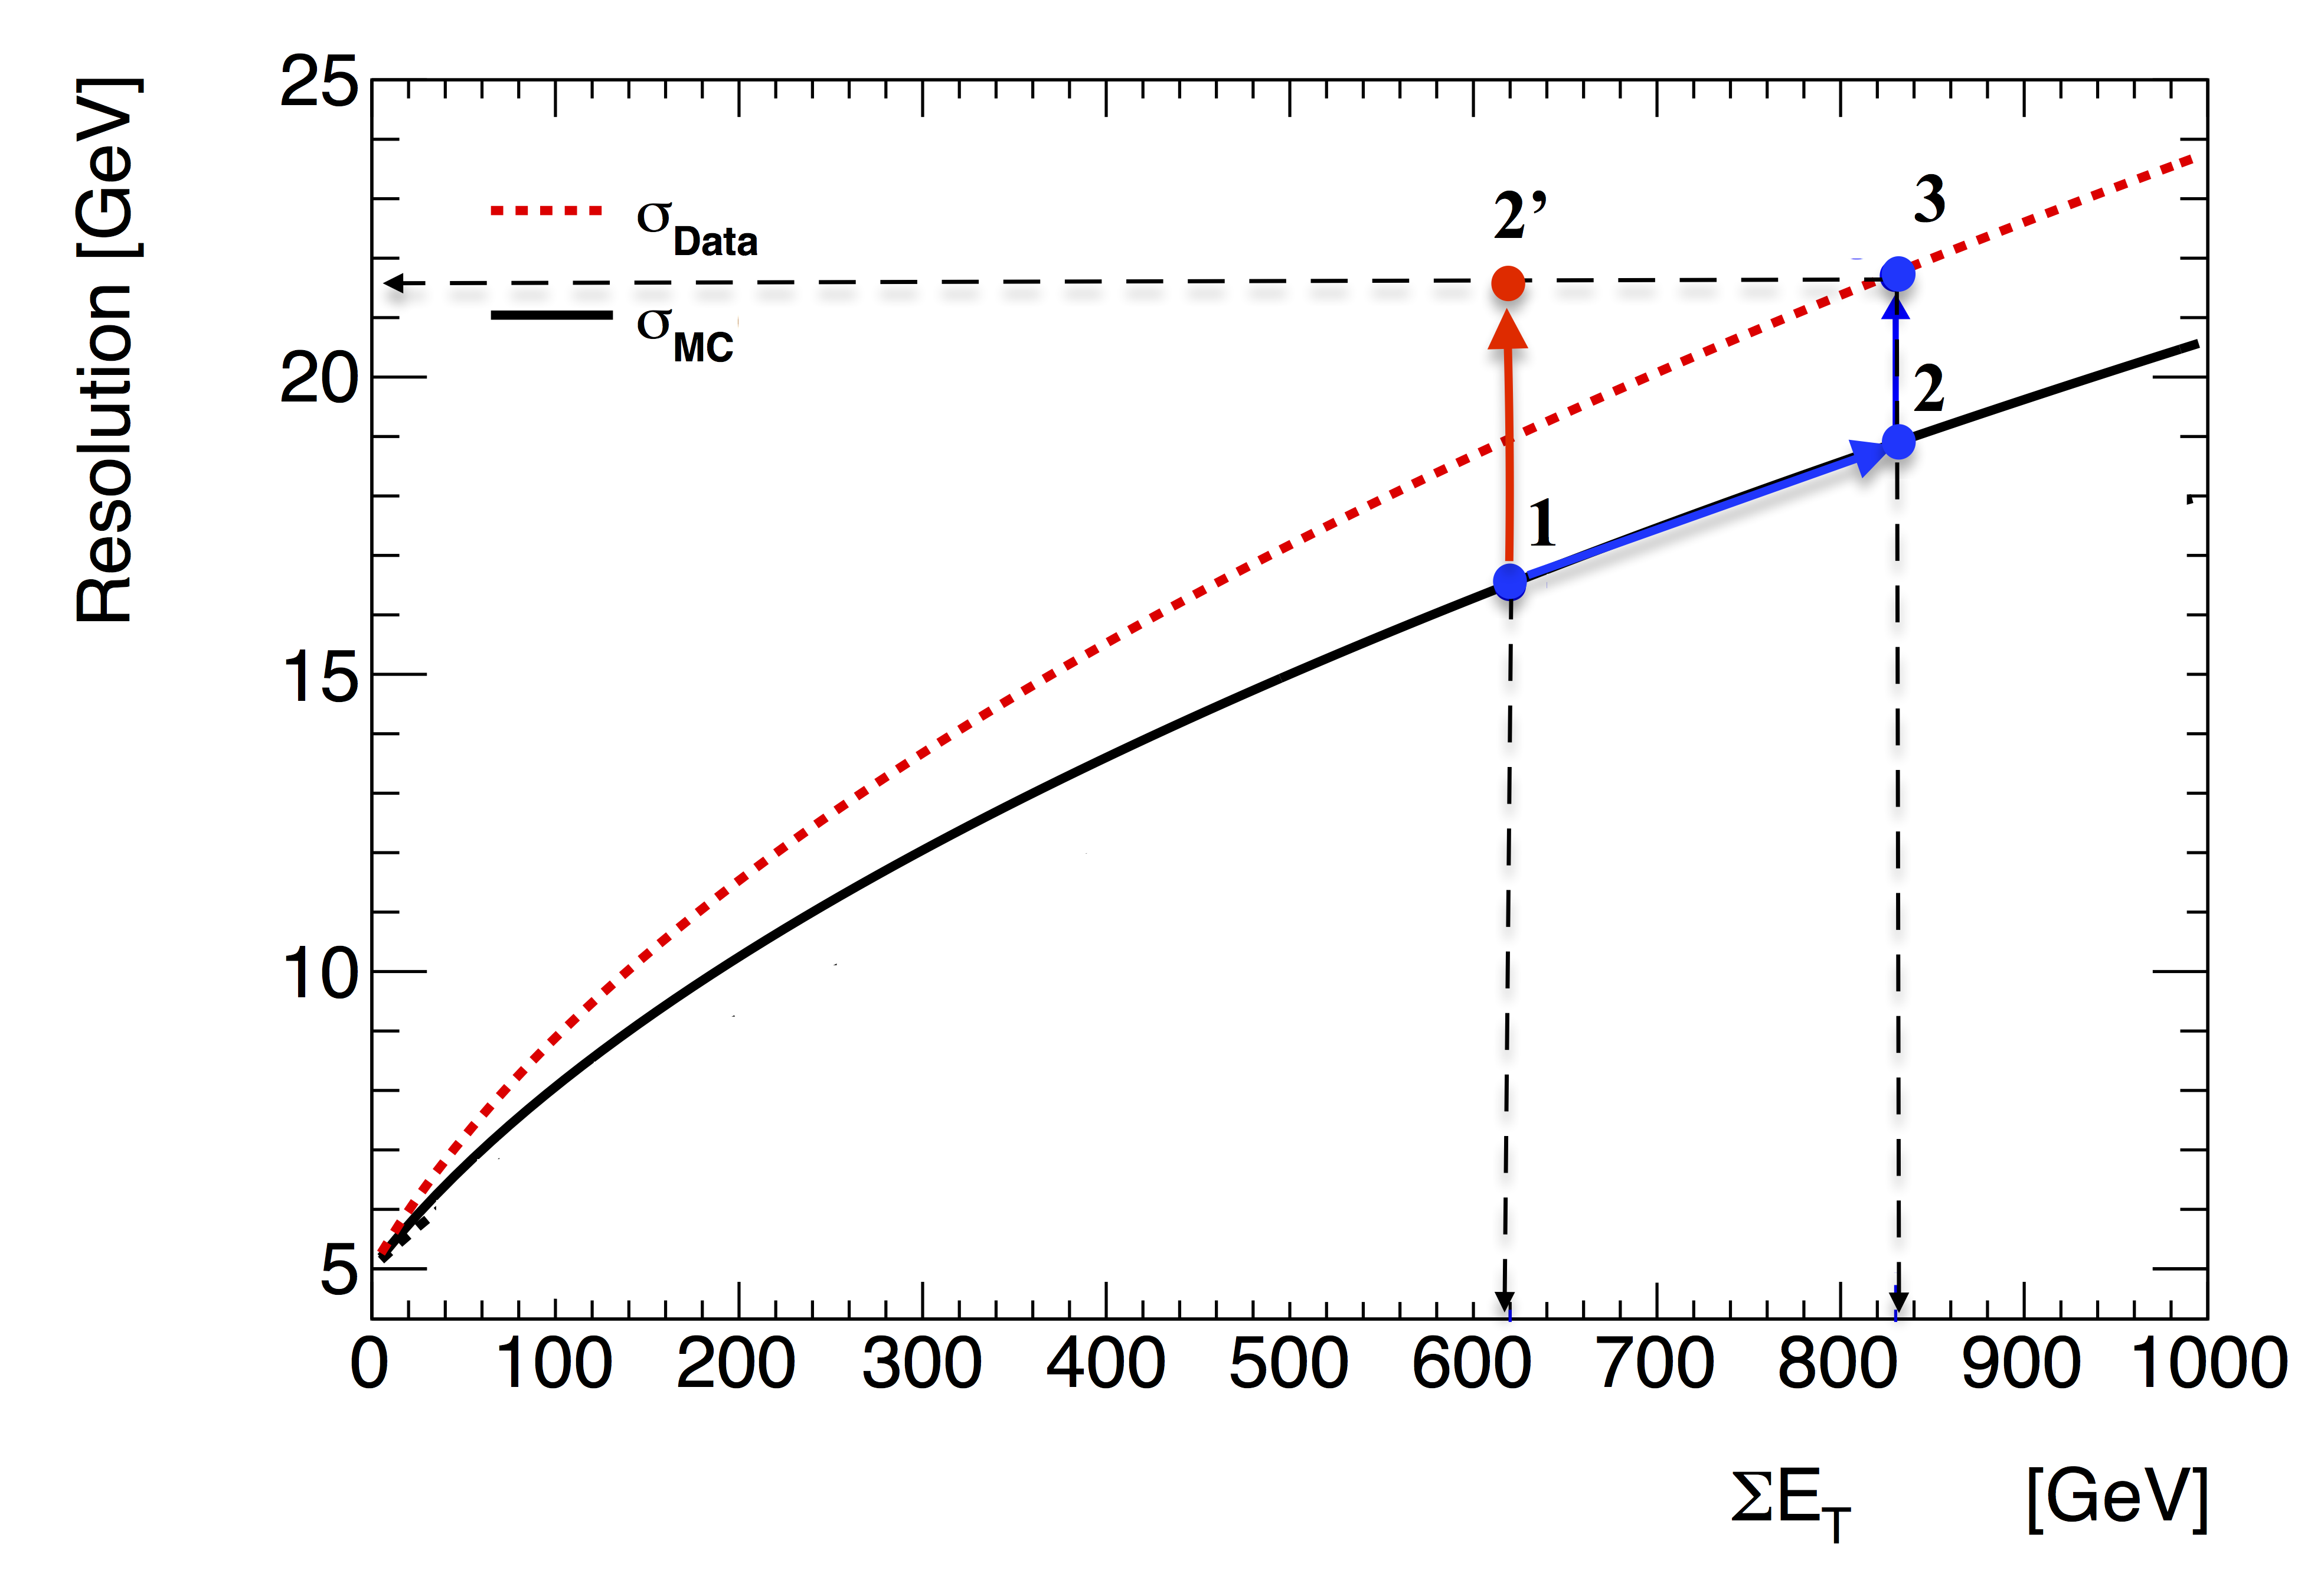
\includegraphics[width=1.\linewidth]{HadronRecoil/sumet.png}}
\end{minipage}

\end{center}
\caption{Schematic view of hadronic recoil correction procedure: this figure illustrates the resolution of \uperp as a function of event activity \sumet. The dotted curve represents \uperp resolution in data($\sigma_{data}$) and the solid black line a nominal \uperp resolution in simulation ($\sigma_{MC}$). Modified from \cite{HRCorrections}.}

\label{ris:sumetCor}
\end{figure}


The event activity plays an important role in the \etmiss reconstruction. Since \sumet and the hadronic recoil are correlated, the possible mismodelling of the event activity can lead to differences between the data and the Monte Carlo \etmiss resolution. There are two ways to correct the resolution (Fig.~\ref{ris:sumetCor}):
\begin{itemize}
\item A two-step procedure, shown as path 1-2-3 in Fig.~\ref{ris:sumetCor}. In the first step, the \sumet distribution in the simulation is corrected to match the data. In the second step, the remaining differences in hadronic recoil resolution between data and simulation are corrected.
\item As a one-step procedure, there the second order effects on \etmiss coming from \sumet modeling are neglected and the resolution differences between data and MC corrected directly. This procedure is shown as the path 1-2' in Fig.~\ref{ris:sumetCor}.
\end{itemize}
Both methods of hadronic recoil resolution correction are described in the following sections

\subsection{Event activity correction}\label{sec:SumetCor}



\begin{figure}[!tbp]
\begin{minipage}[h]{0.49\linewidth}
\center{\includegraphics[width=1.\linewidth]{HadronRecoil/UncorrSumet/W_EtMiss_CorRecoilSumet.pdf} \\ a)}
\end{minipage}
\hfill
\begin{minipage}[h]{0.49\linewidth}
\center{\includegraphics[width=1.\linewidth]{HadronRecoil/UncorrSumet/Wmu_EtMiss_CorRecoilSumet.pdf} \\ b)}
\end{minipage}
\caption{\sumet distribution from a) the \wenu and b) the \wmunu analysis selection.}
\label{HadrRecoil:UncorrSumet}
\end{figure}

\begin{figure}[!tbp]
\begin{minipage}[h]{0.49\linewidth}
\center{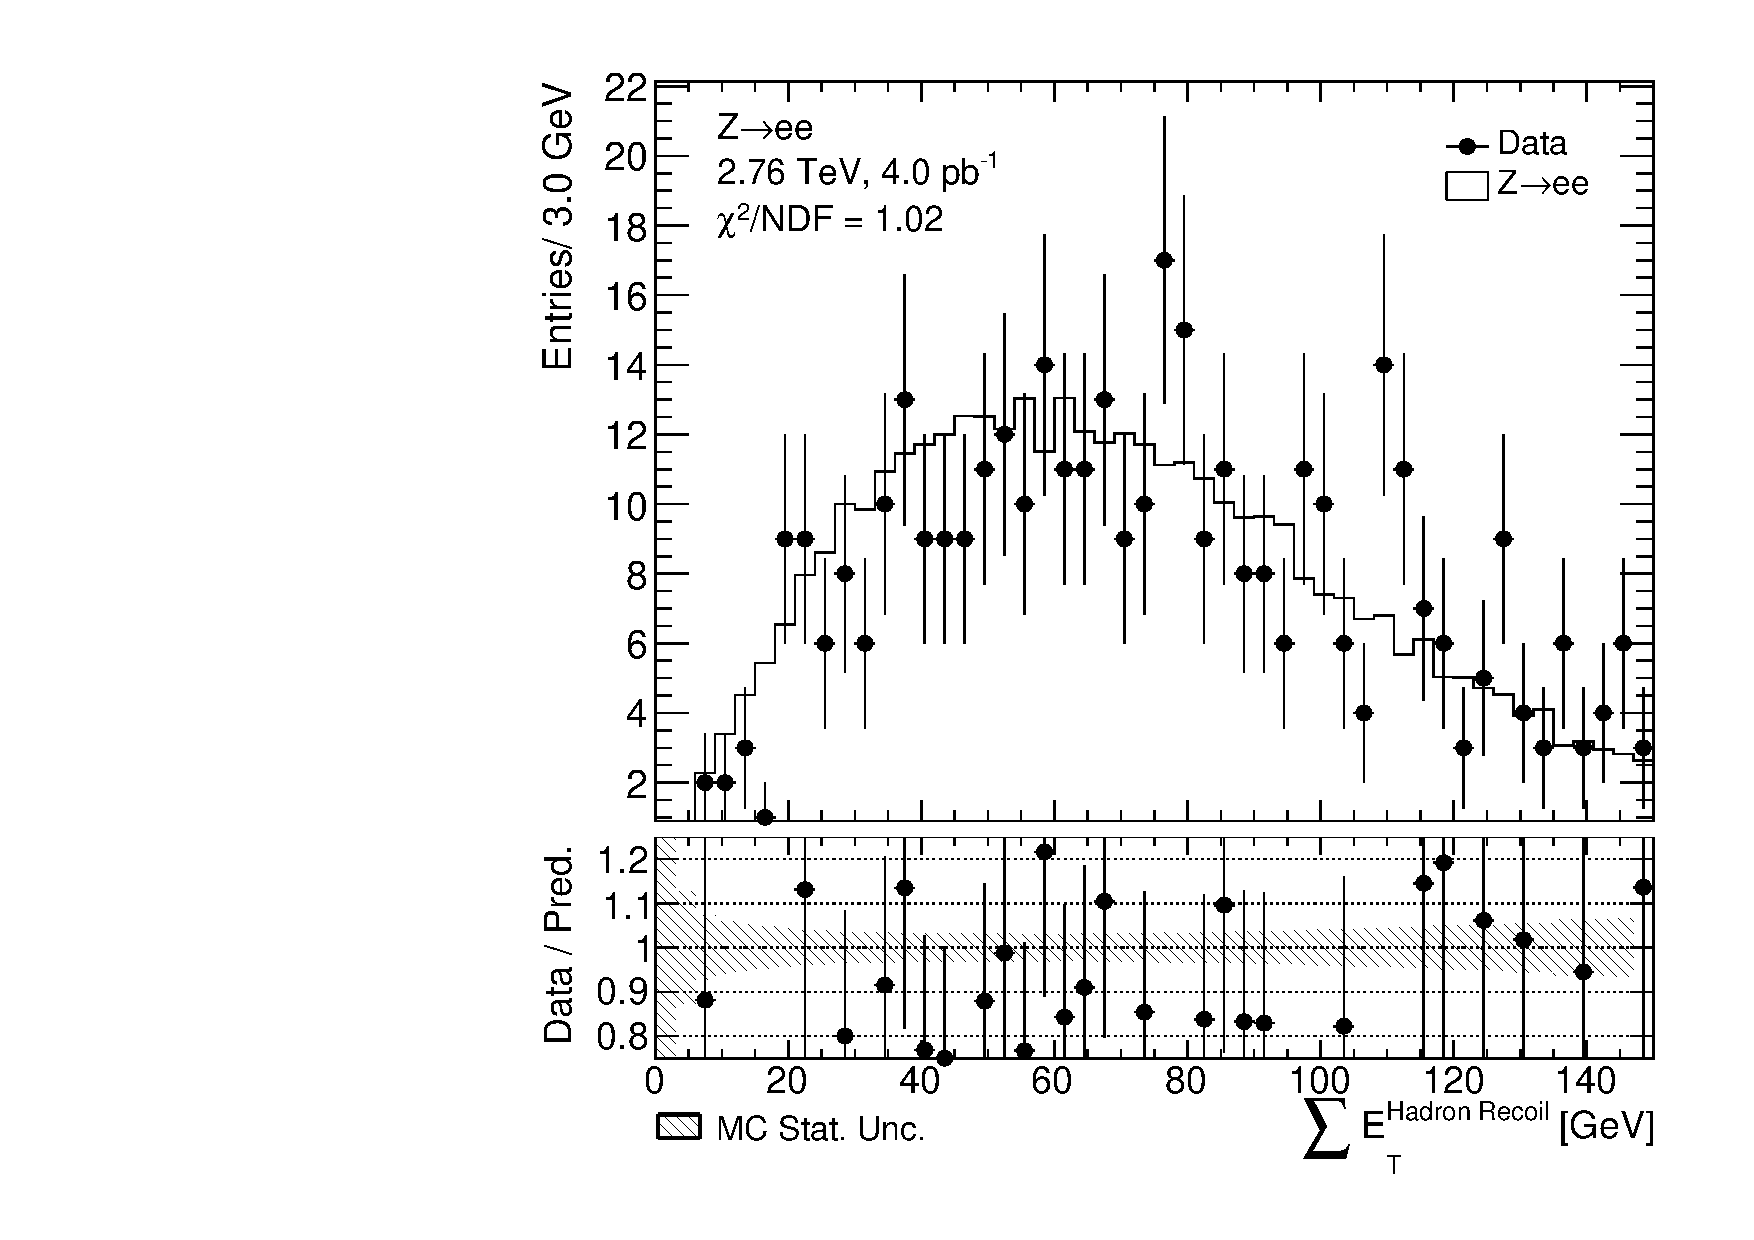
\includegraphics[width=1.\linewidth]{HadronRecoil/ZeeSumet.pdf} \\ a)}
\end{minipage}
\hfill
\begin{minipage}[h]{0.49\linewidth}
\center{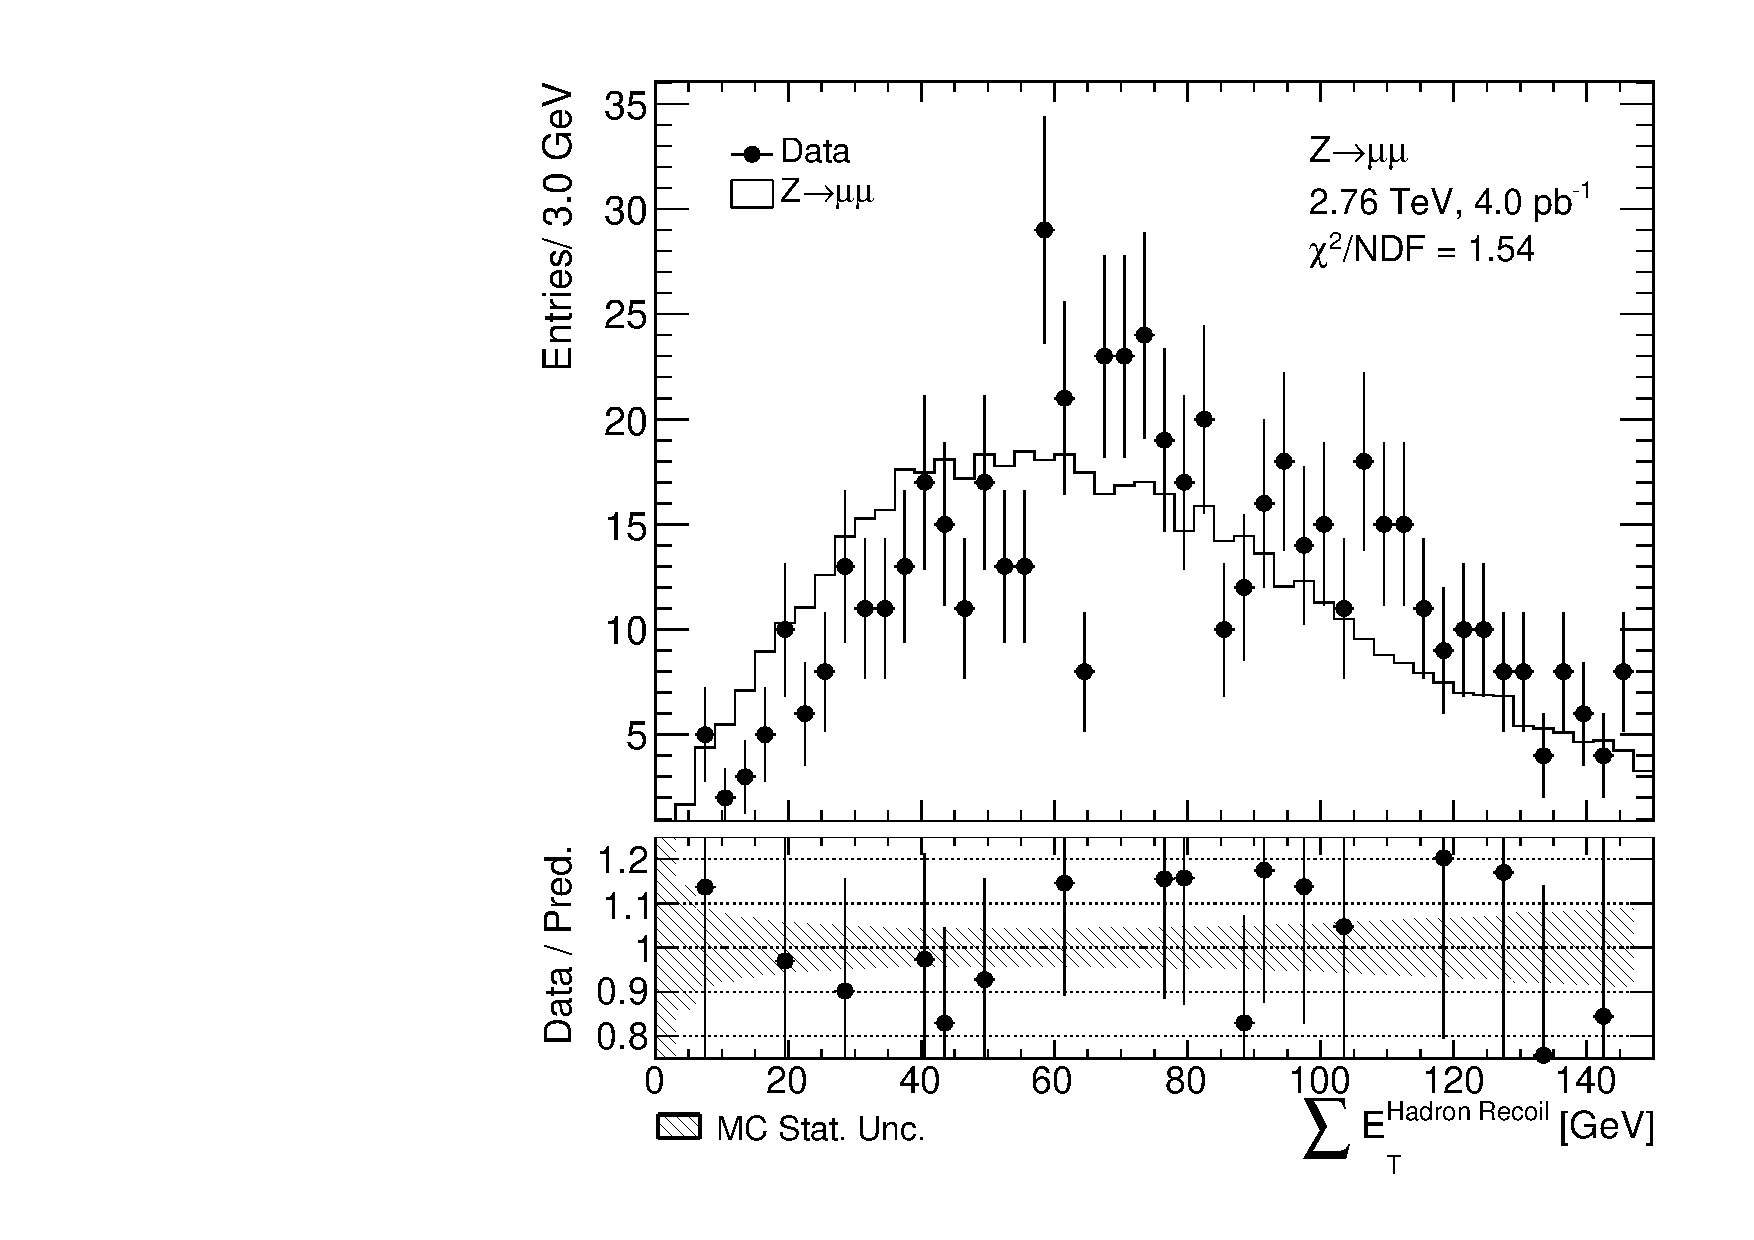
\includegraphics[width=1.\linewidth]{HadronRecoil/ZmumuSumet.pdf} \\ b)}
\end{minipage}
\caption{\sumet distribution from a) the $Z\to ee$  and b) the $Z\to \mu\mu$ analysis selection.}
\label{HadronRecoilSumetZ}
\end{figure}

\begin{figure}[!tb]
\center{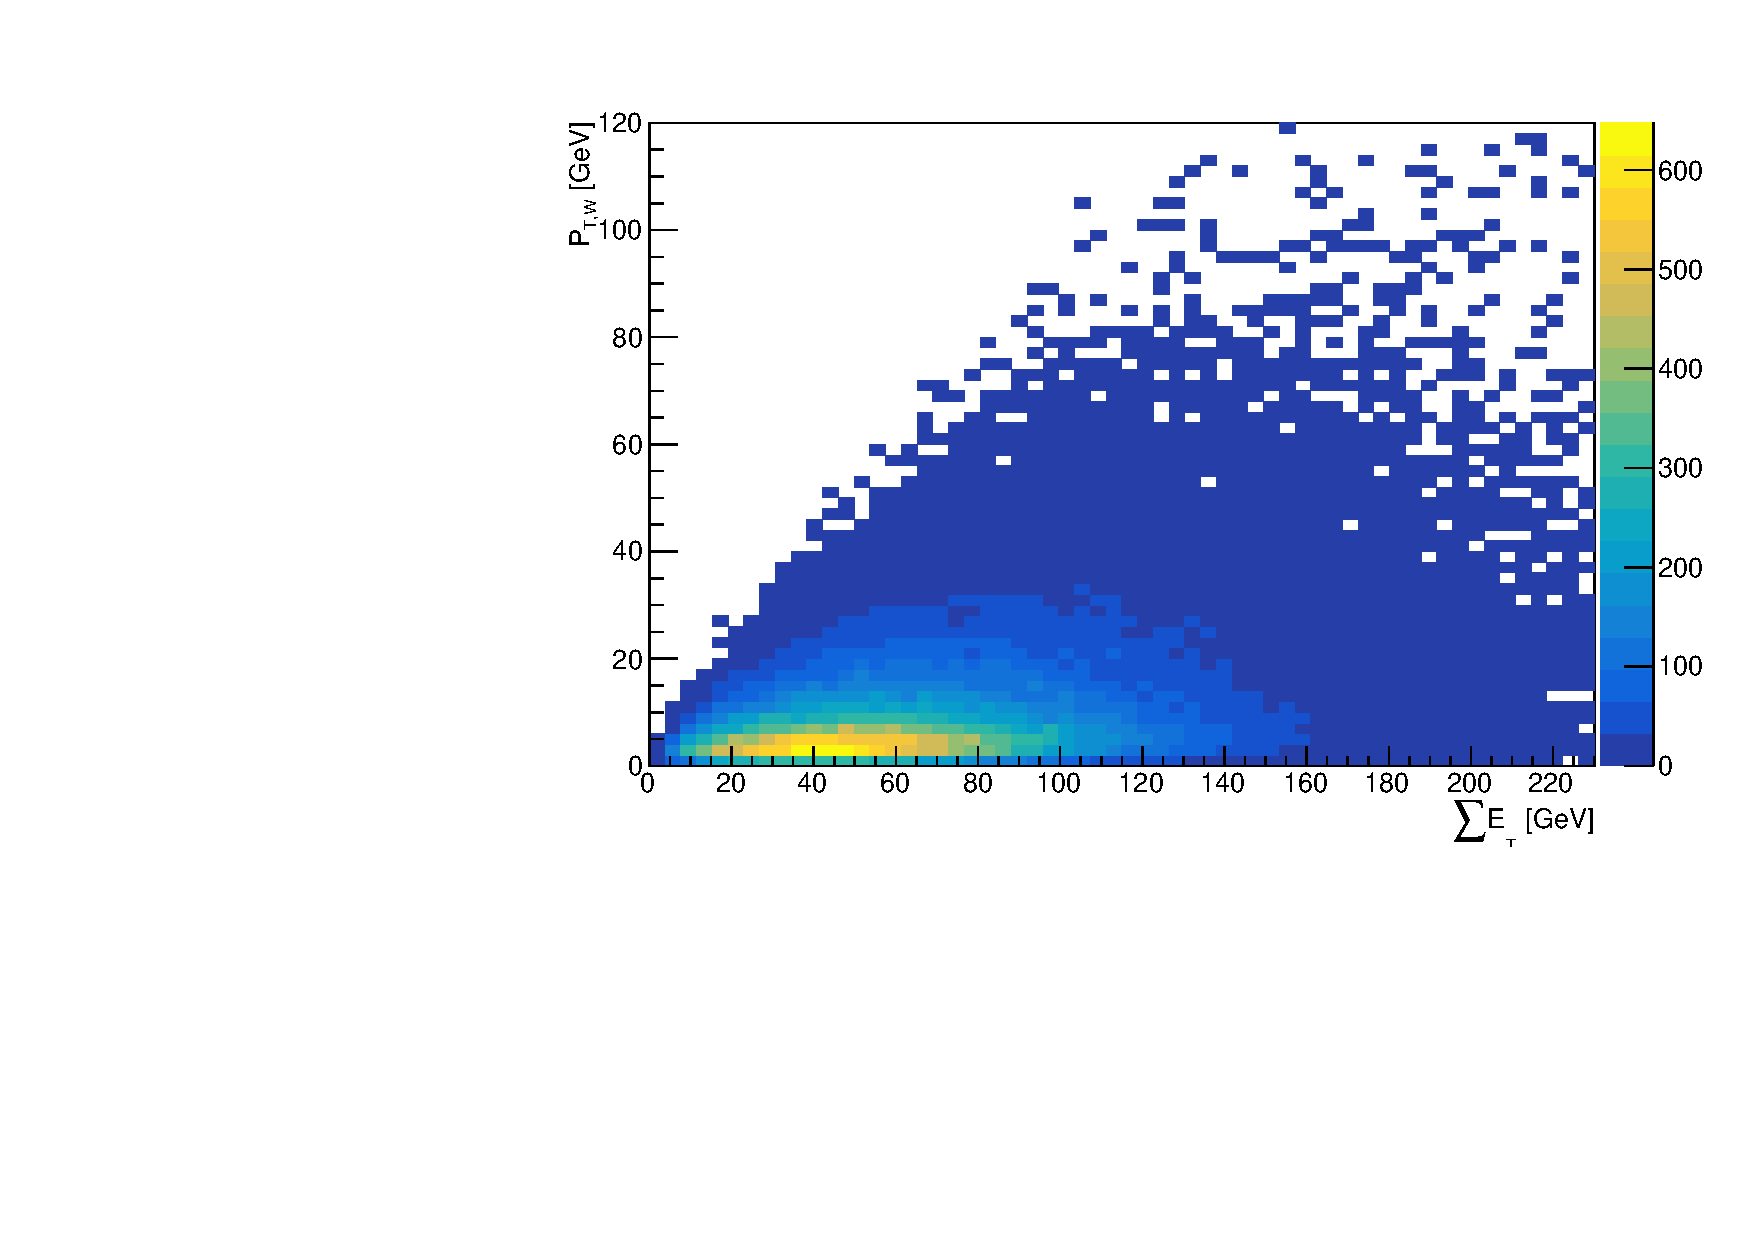
\includegraphics[width=0.9\linewidth]{HadronRecoil/SumetPtTruth.pdf} }
\caption{Distribution of \sumet vs true transverse momentum of the W boson (\ptw$^{truth}$) in the $W^{+} \to e^{+}\nu$ MC sample.  }
\label{HadrRecoil:SumetPt}
\end{figure}




The distributions of event activity are shown in Fig.~\ref{HadrRecoil:UncorrSumet}. A visible shift between the data and the MC distribution for both W boson channels is observed. The standard procedure of hadronic recoil resolution correction (used in the \mtw measurement at 7 TeV) uses a Smirnov transformation applied on simulated events from the \sumet and $P_{T}^{bos}$ distributions in events containing a Z-boson candidates \cite{HRCorrections}. Distribution of the event activity in the Z-boson candidate events is shown in Fig.~\ref{HadronRecoilSumetZ}. The discrepancies between data and simulation are not visible using the \chiD-test, therefore this procedure cannot be adapted for the $\sqrt{s}$ = 2.76 TeV data, therefore the W-boson candidate events are used to determine the event activity correction.

\begin{figure}[!tbp]
\begin{minipage}[h]{0.49\linewidth}
\center{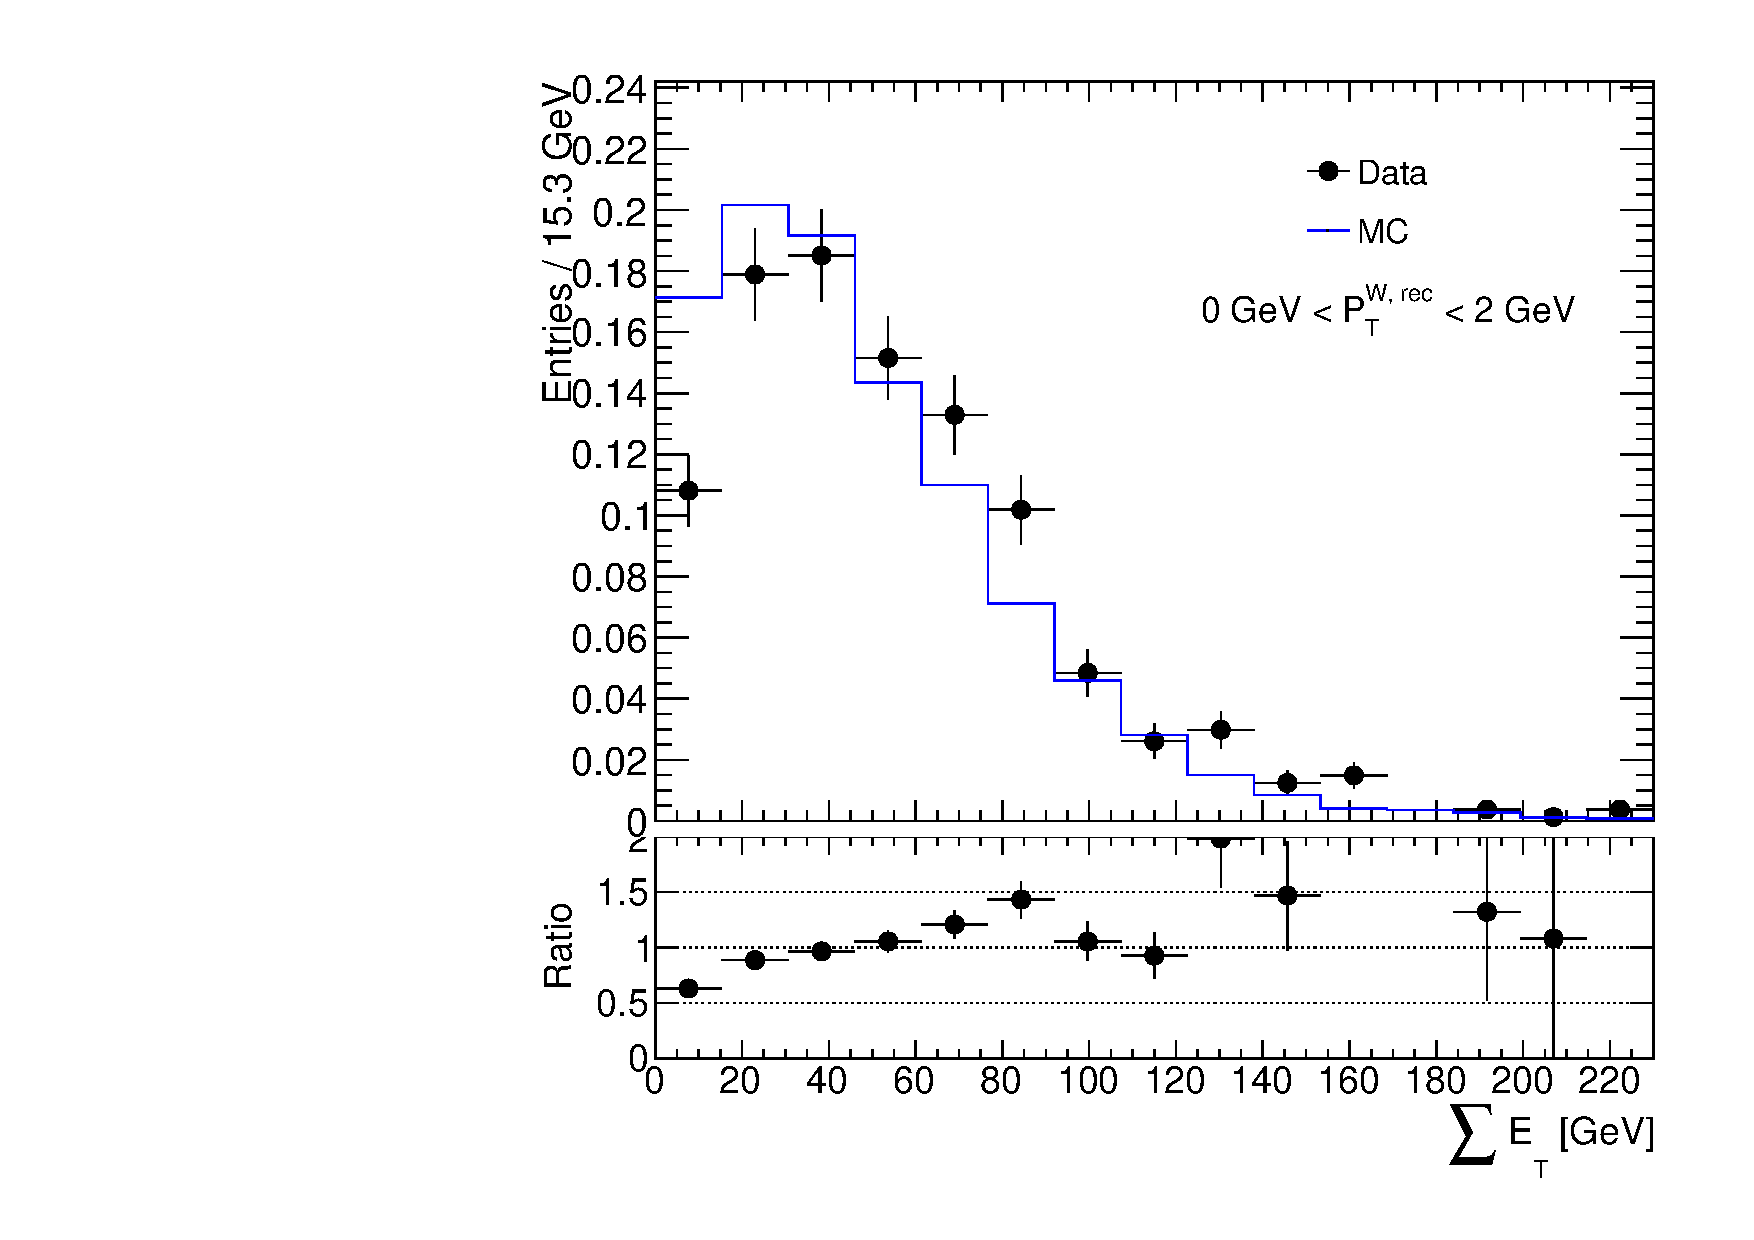
\includegraphics[width=1.\linewidth]{HadronRecoil/2.pdf} \\ a)}
\end{minipage}
\hfill
\begin{minipage}[h]{0.49\linewidth}
\center{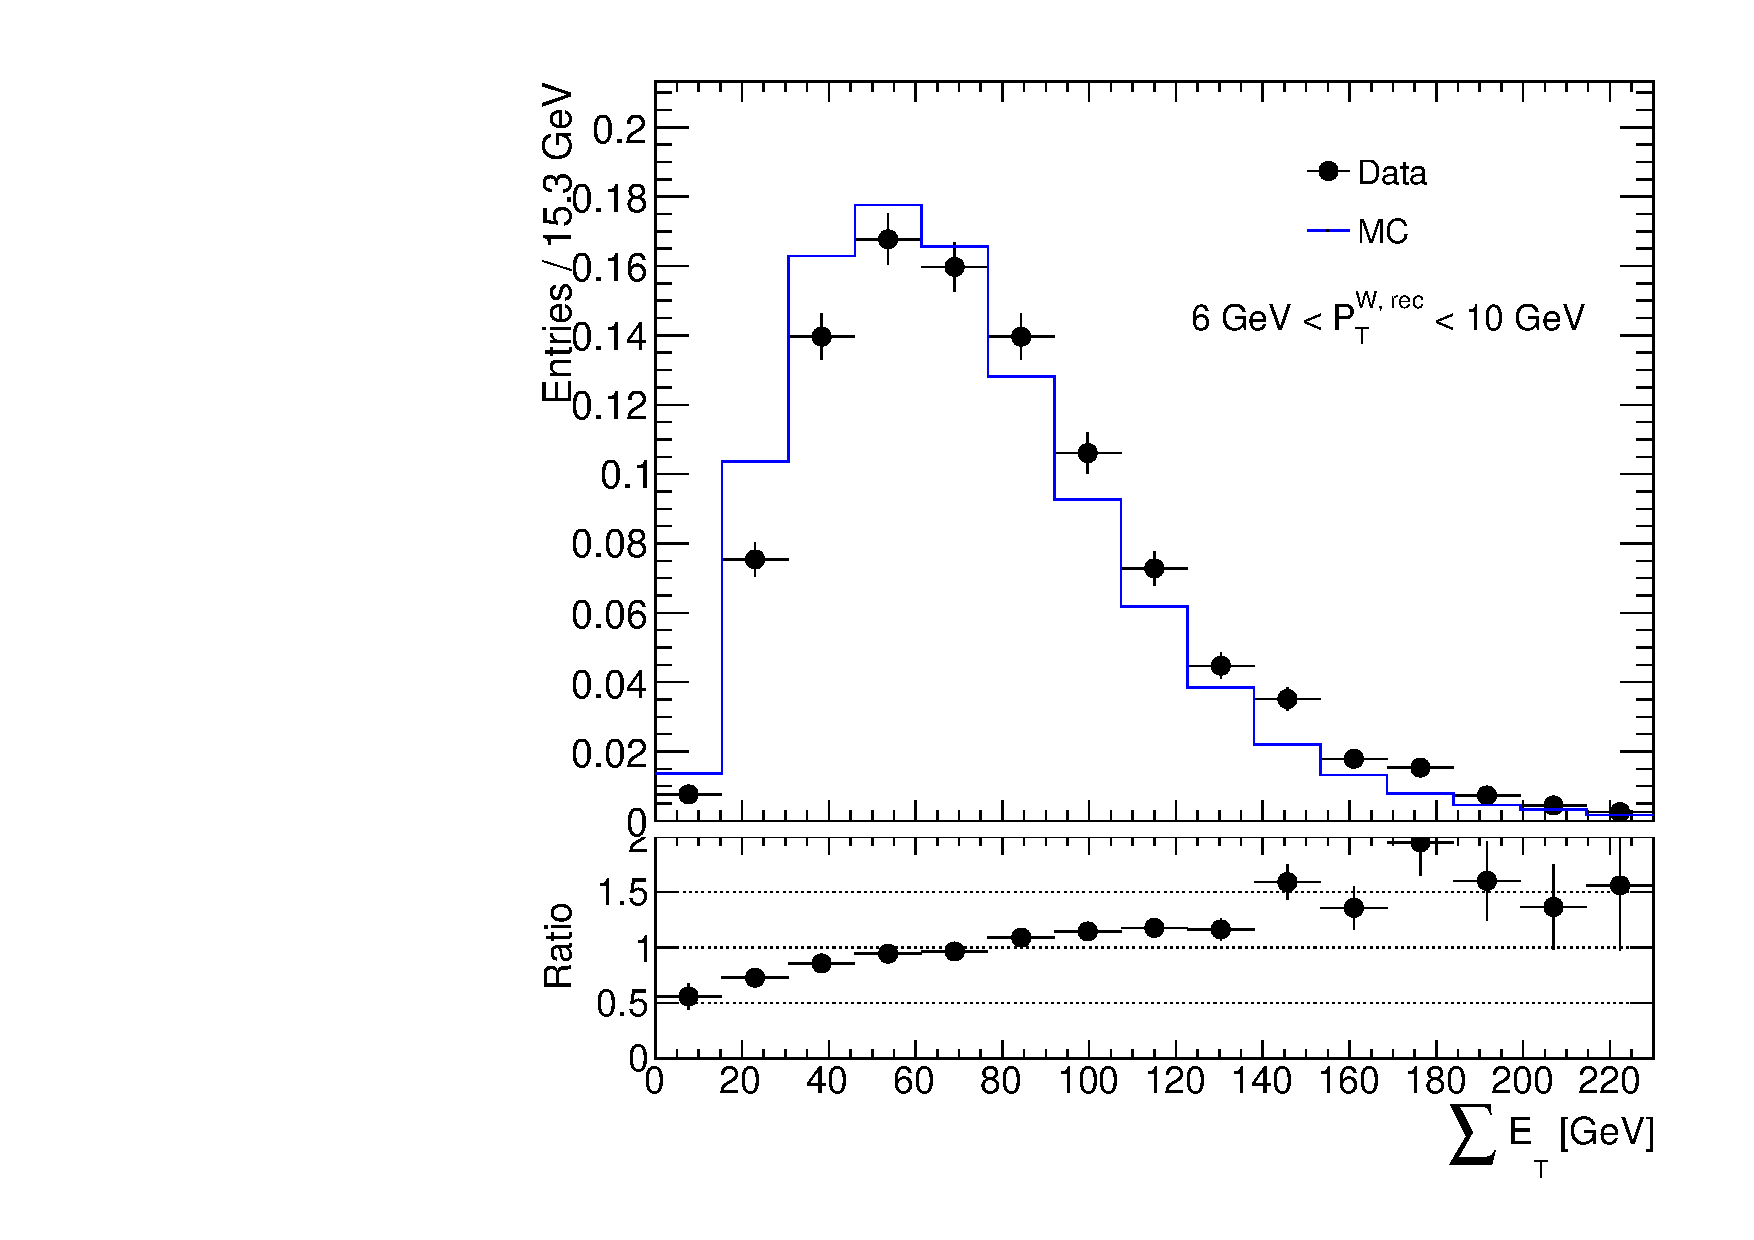
\includegraphics[width=1.\linewidth]{HadronRecoil/10.pdf} \\ b)}
\end{minipage}
\caption{\sumet distribution for the a) $P_T^{W, rec}$ < 2 GeV b) 6 GeV < $P_T^{W, rec}$ < 10 GeV .}
\label{ris:SumEtCorPtW}
\end{figure}


The event activity \sumet is correlated to the truth transverse momentum of the boson, as shown in Fig.~\ref{HadrRecoil:SumetPt}.  In order to avoid a bias introduced in \ptw spectrum by the reweighting , the reweighting constant are considered as a function of reconstructed W-boson transverse momentum $P_T^{W, rec}$. For each $P_T^{W, rec}$ bin the reweighting constants are calculated as:
\begin{equation}
SF^{channel}=\frac{\sum E_T^{data, \, selection} }{\sum E_T^{MC,\, no\, selection} },
\end{equation}
where $\sum E_T^{data,\, selection} $ is a \sumet distribution inside a given $P_T^{W, rec}$ for events satisfying the full event selection. The second term, $\sum E_T^{MC,\, no\, selection}$, stands for \sumet distribution in MC before applying event selection. The total number of $P_T^{W, rec}$ bins is 6. The scale factor are applied as a reconstructed weight on simulated events.

Distribution of \sumet for two different $P_T^{W, rec}$ regions is shown in Fig.\ref{ris:SumEtCorPtW}. The determined reweighting constants for \wenu and \wmunu MC samples are shown in Fig.~\ref{ris:SumEtCorNoPol}. The \sumet distribution after the correction is shown in Fig.~\ref{HadrRecoil:CorrSumet}. This correction has almost no effect the reconstructed transverse momentum distribution and introduces only a small change in the truth boson spectrum, as shown in Fig.~\ref{HadrRecoil:PtSpectrum}. 


\begin{figure}[!tbp]
\begin{minipage}[h]{0.49\linewidth}
\center{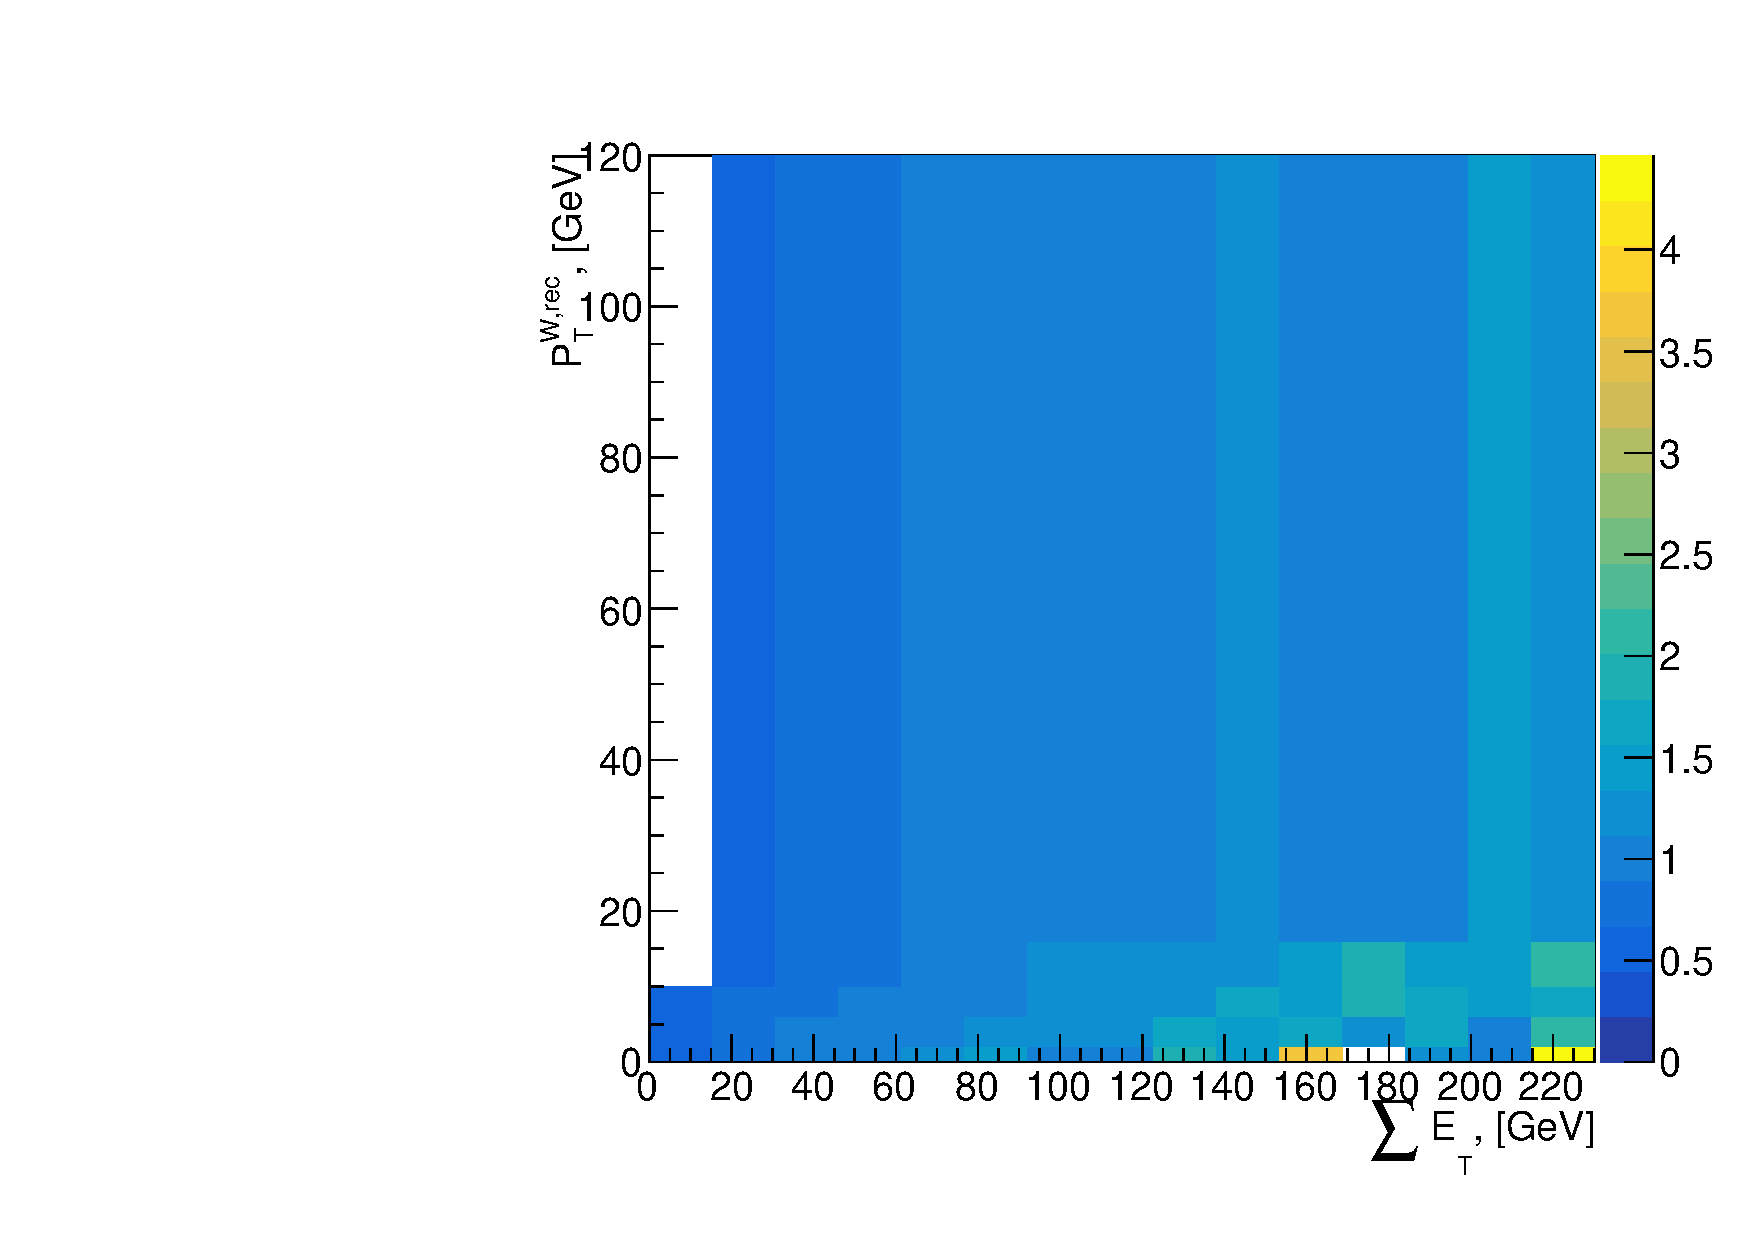
\includegraphics[width=1.\linewidth]{HadronRecoil/ReweightingNoPolEP.pdf} \\ a)}
\end{minipage}
\hfill
\begin{minipage}[h]{0.49\linewidth}
\center{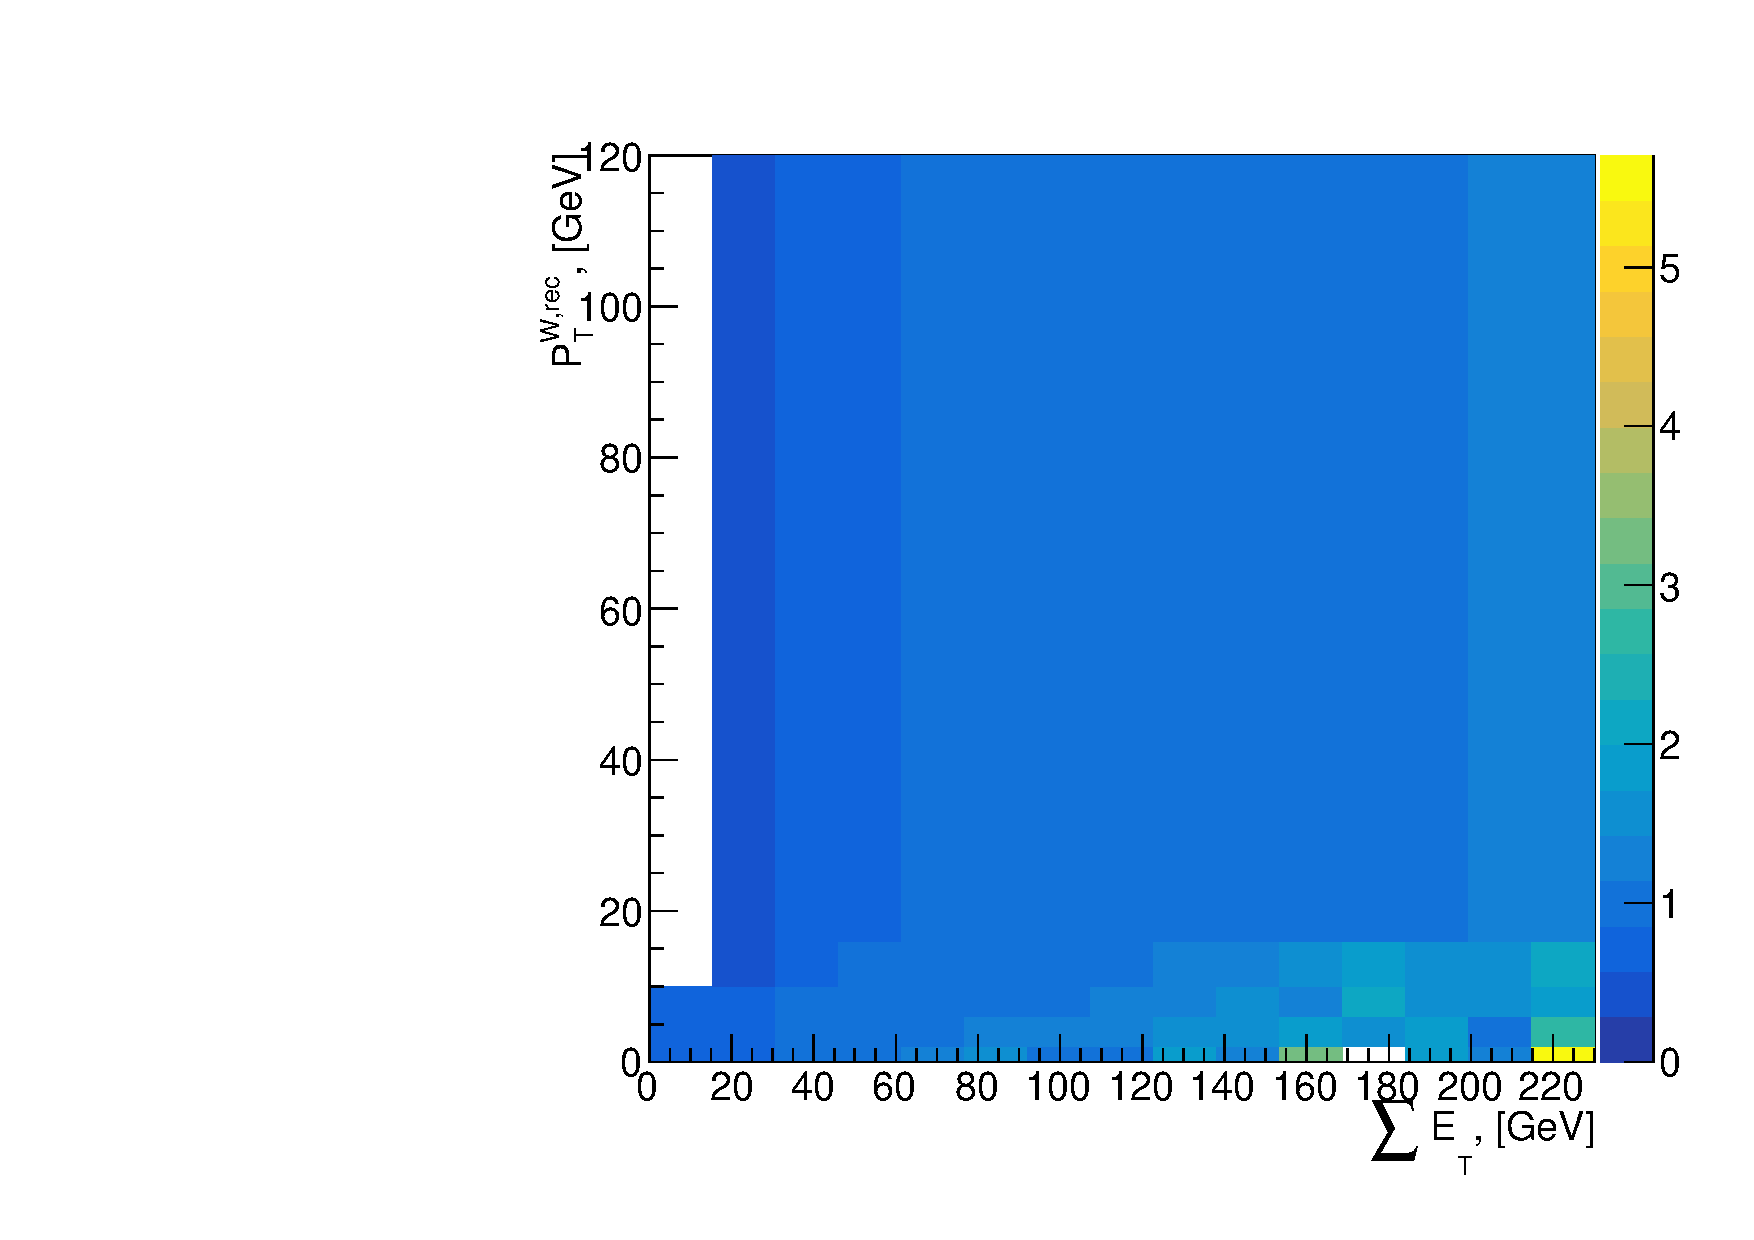
\includegraphics[width=1.\linewidth]{HadronRecoil/ReweightingNoPolMP.pdf} \\ b)}
\end{minipage}
\caption{\sumet reweighting constants derived for a) $W^{+} \to e \nu$ and b) $W^{+} \to \mu \nu$ MC sample.}
\label{ris:SumEtCorNoPol}
\end{figure}

\begin{figure}[!tbp]
\begin{minipage}[h]{0.5\linewidth}
\center{\includegraphics[width=1.\linewidth]{HadronRecoil/CorrSumet/W_EtMiss_CorRecoilSumet.pdf} \\ a)}
\end{minipage}
\hfill
\begin{minipage}[h]{0.5\linewidth}
\center{\includegraphics[width=1.\linewidth]{HadronRecoil/CorrSumet/Wmu_EtMiss_CorRecoilSumet.pdf} \\ b)}
\end{minipage}
\caption{\sumet distribution from a) the \wenu and b) the \wmunu analysis channels after applying \sumet correction. }
\label{HadrRecoil:CorrSumet}
\end{figure}

\begin{figure}[!tbp]
\begin{minipage}[h]{0.49\linewidth}
\center{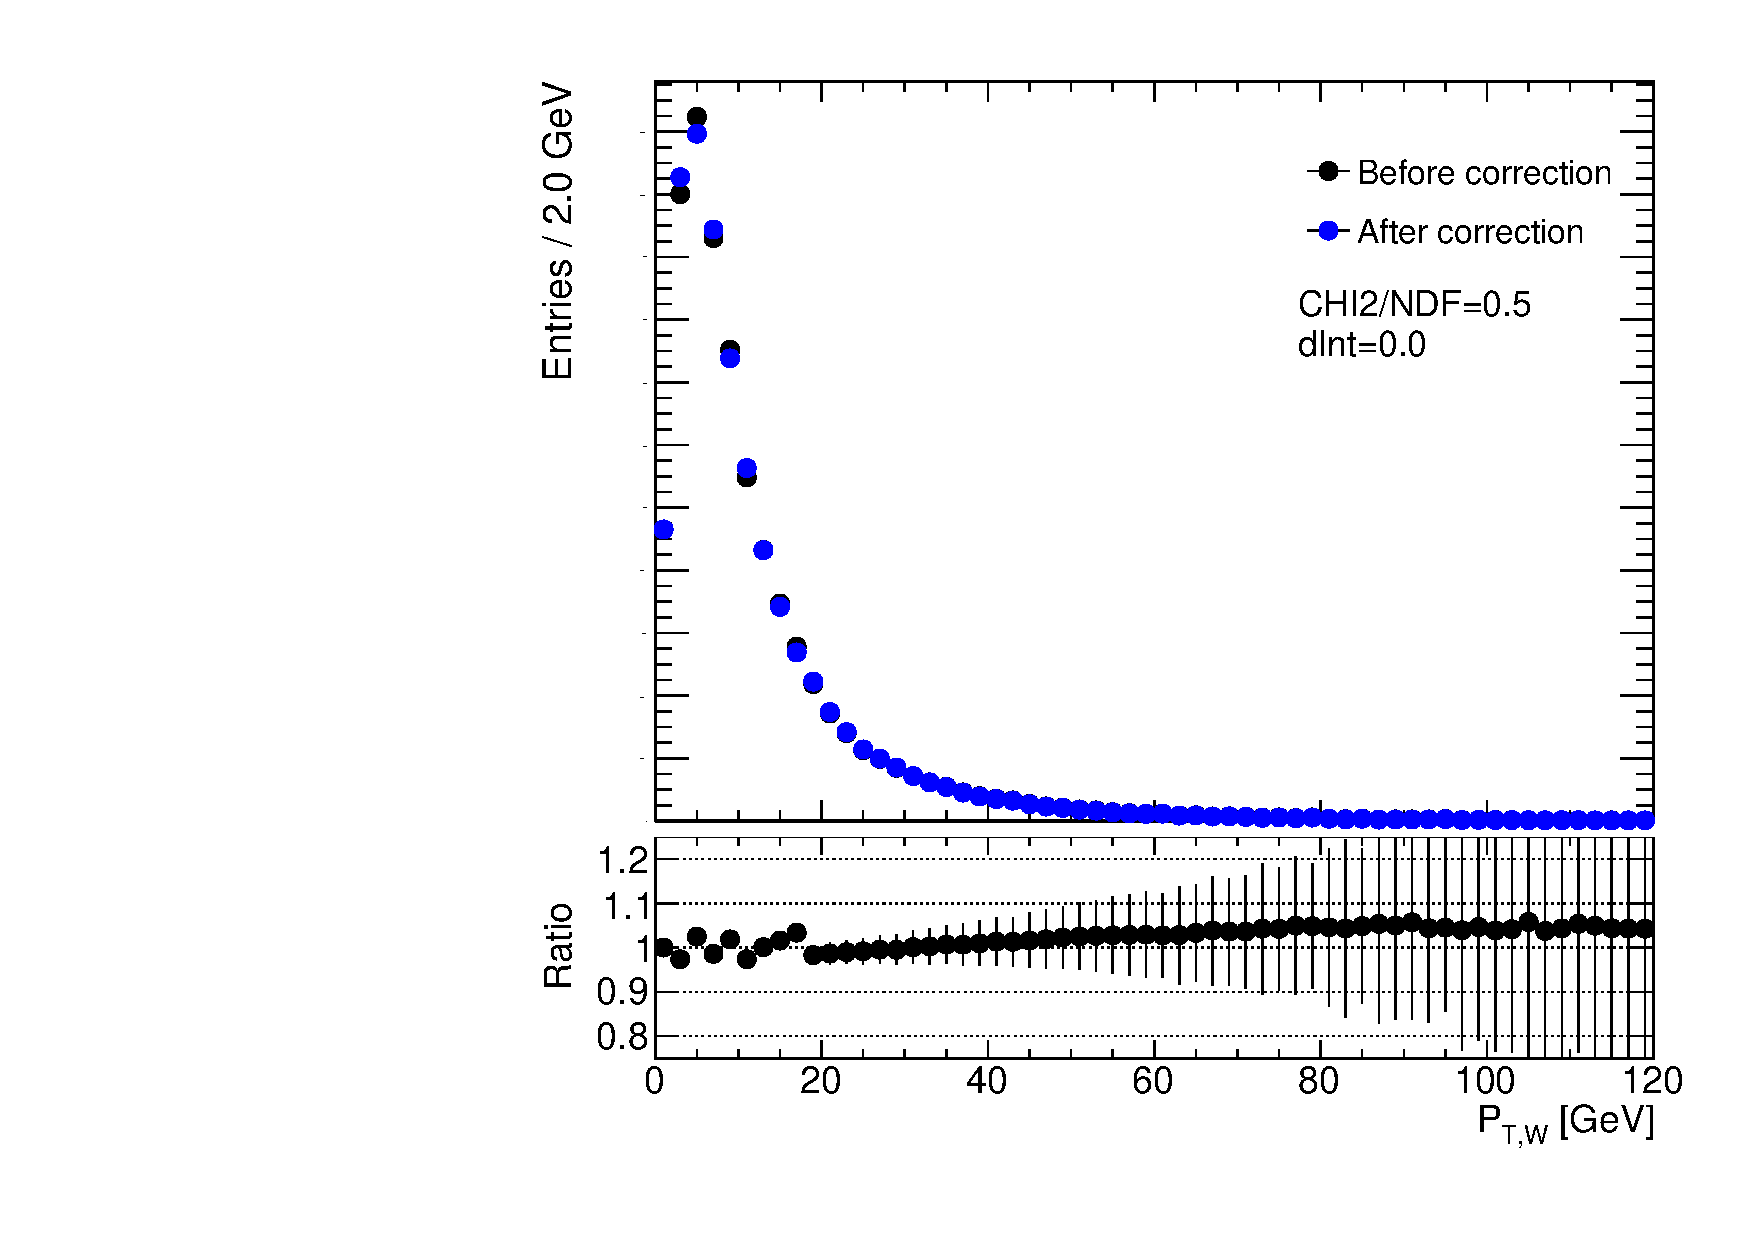
\includegraphics[width=1.\linewidth]{HadronRecoil/WplusenuRecoEffect.pdf} \\ a)}
\end{minipage}
\hfill
\begin{minipage}[h]{0.49\linewidth}
\center{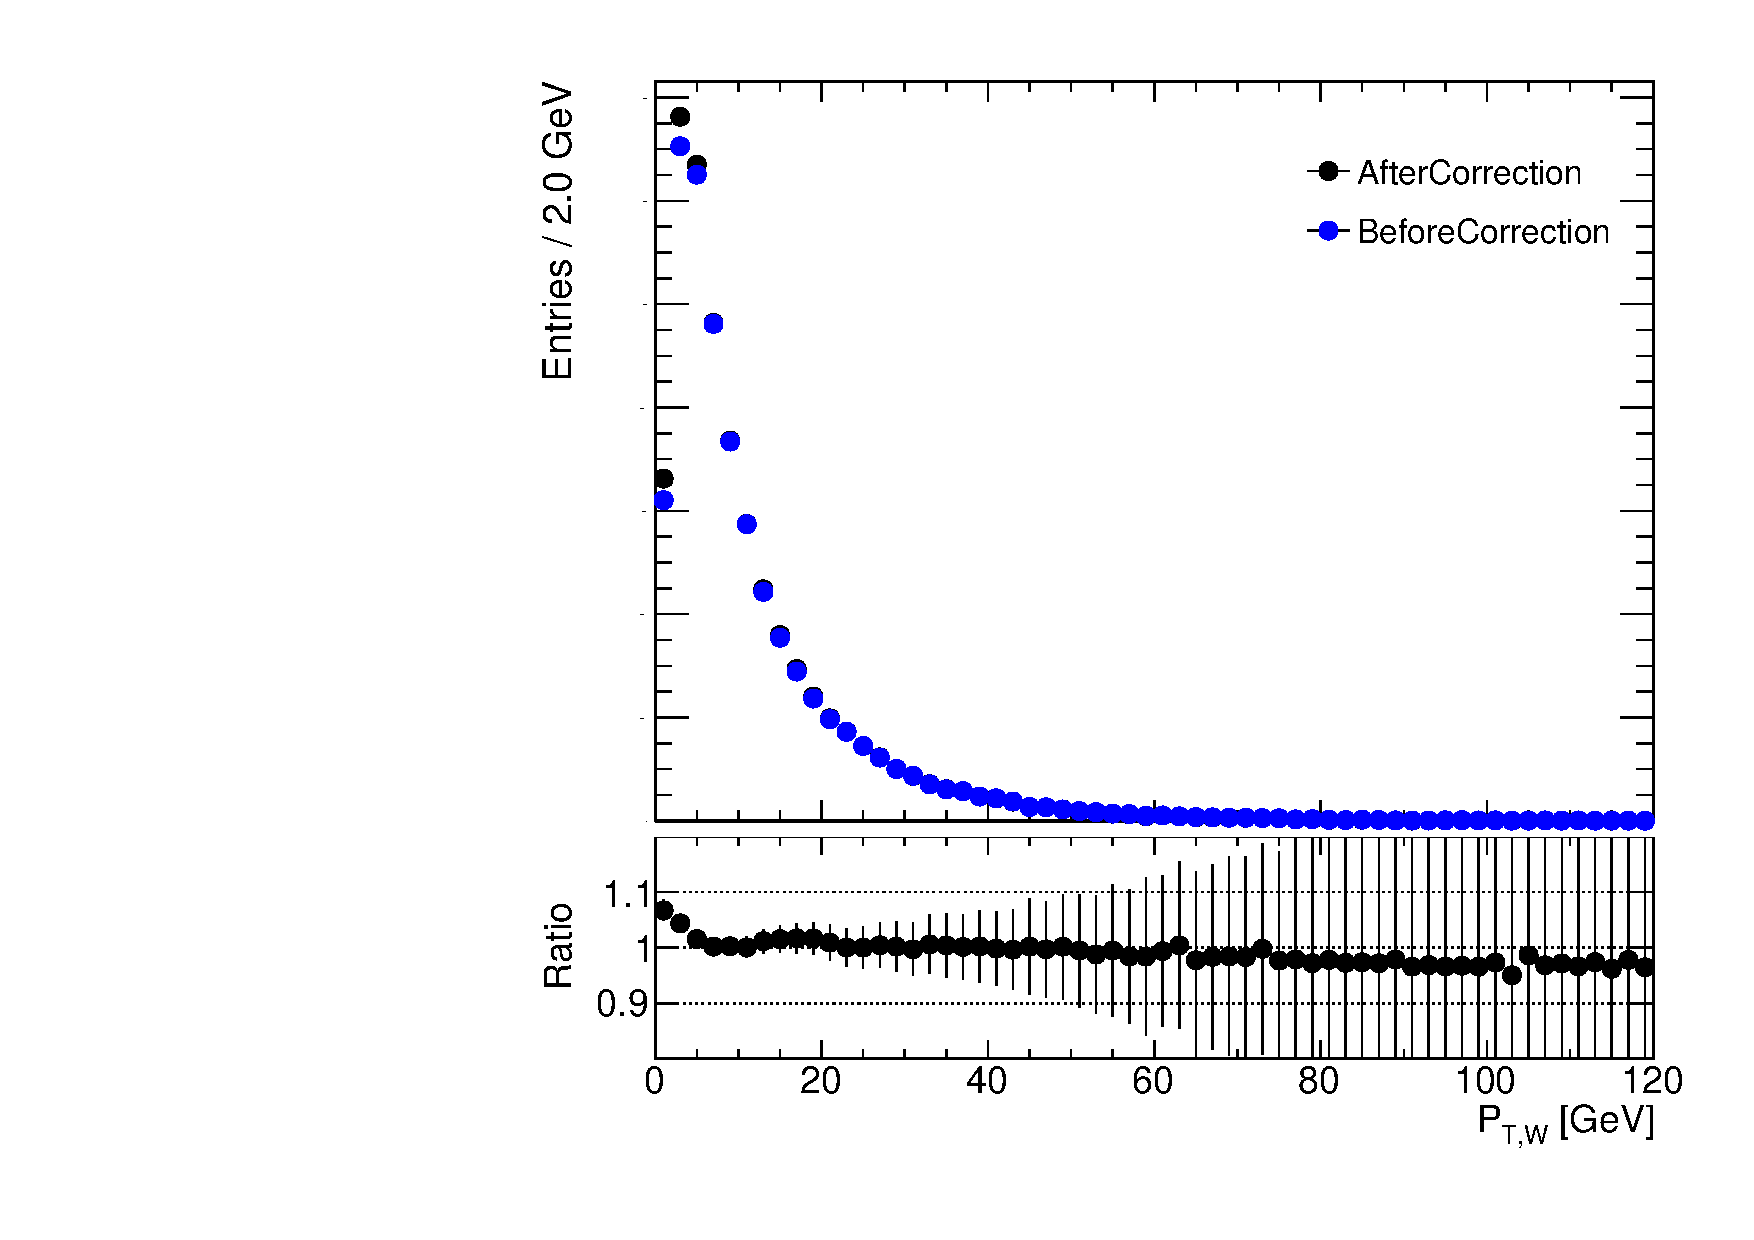
\includegraphics[width=1.\linewidth]{HadronRecoil/Wplusenu.pdf} \\ b)}
\end{minipage}
\caption{Effect of the \sumet reweighting on a) reconstructed transverse momentum of the boson and b) truth transverse momentum of the W-boson.}
\label{HadrRecoil:PtSpectrum}
\end{figure}

\subsubsection{Method cross-check}

The method can be cross-checked using the approximation of the correction constants by a polynomial degree 2 or 1 using the $\chiD$-fit \cite{Watson1967}, in which the following quantity is minimized:
\begin{equation}
\chiD (\mu) = \sum_{i=1}^{N} \frac{(y_i - y(x_i , \mu ))^2}{\sigma_i^2},
\end{equation}
where  index $i$ runs over all of the data points ($x_i$, $y_i$), the $\sigma_i$ is the error of the $i$-th measurement, $\mu\in \boldsymbol{R}^{n+1}$ is the fit parameters vector and $y(x_i, \mu)=\mu_0+\mu_1\cdot x_i +... + \mu_n \cdot x_i^n$ in case of polynomial order $n$.
The covariance matrix  $\mathbf{C}$ for the obtained fit parameters is calculated as a derivative of the minimized \chiD function as:
\begin{equation}
C_{ij}=2\Big(\frac{\delta\chiD}{\delta \mu_i \delta \mu_j} \Big)^{-1}.
\end{equation}

This method allows removing effects related to the data fluctuations, especially for the high \sumet regions (with a low number of events). The reweighting constants after applying smoothing procedure are shown in Fig.~\ref{ris:SumEtCorPol}. 

\begin{figure}[!tbp]
\begin{minipage}[h]{0.49\linewidth}
\center{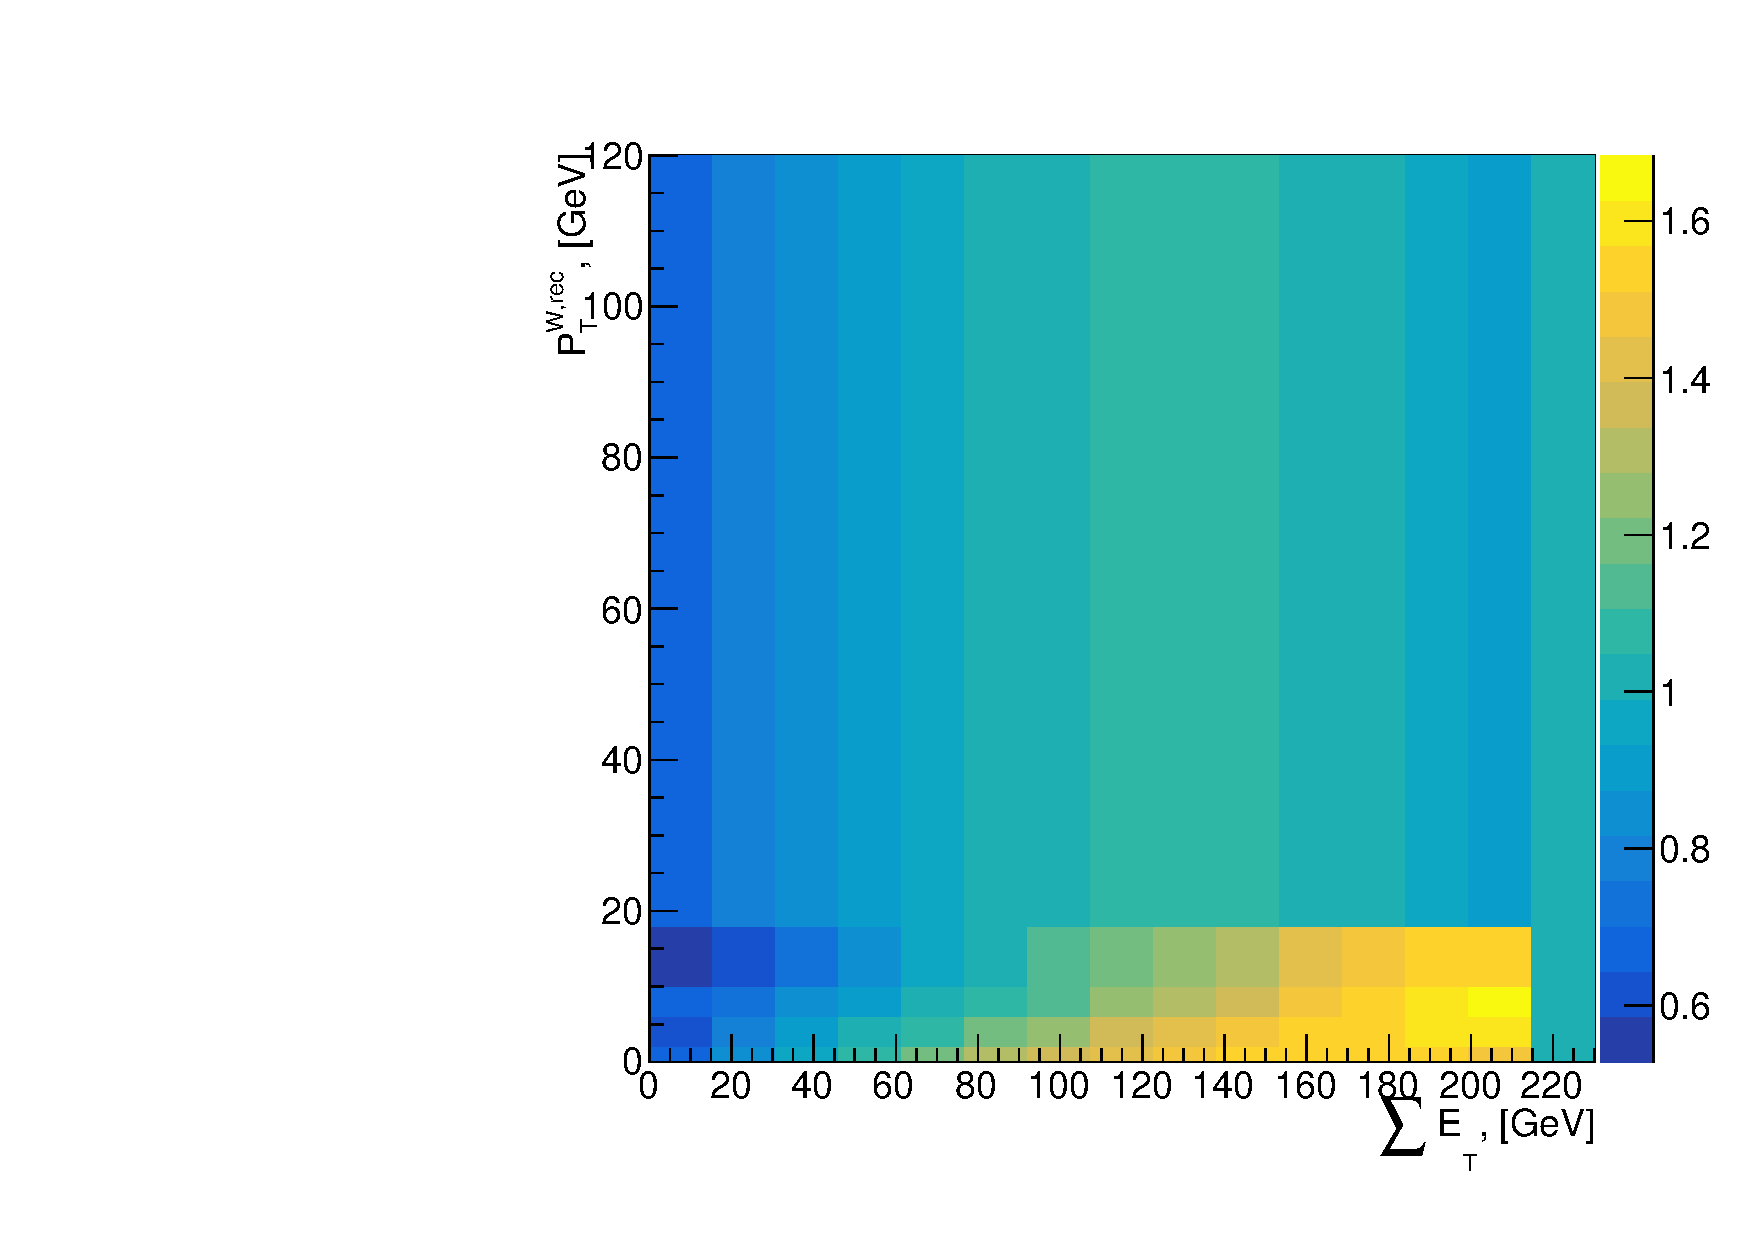
\includegraphics[width=1.\linewidth]{HadronRecoil/ReweightingPolEP.pdf} \\ a)}
\end{minipage}
\hfill
\begin{minipage}[h]{0.49\linewidth}
\center{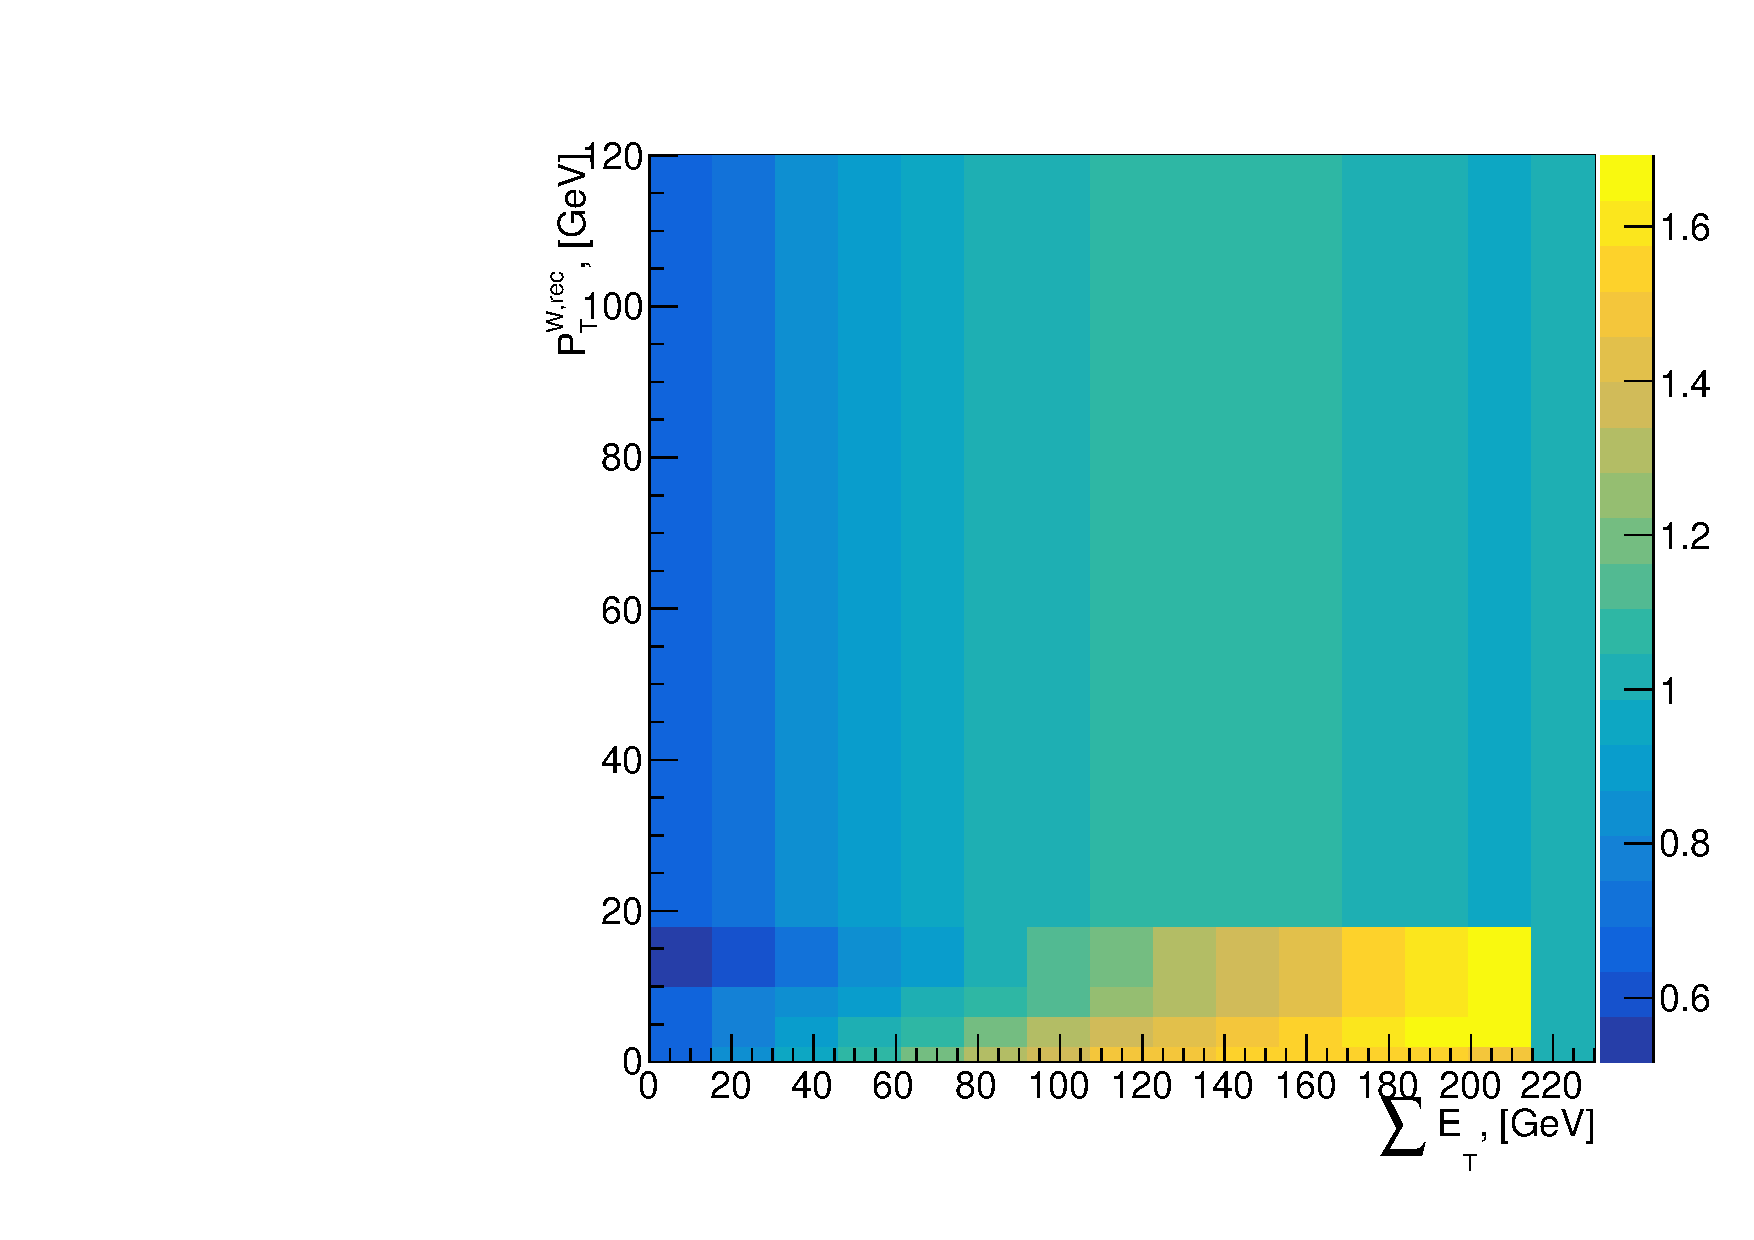
\includegraphics[width=1.\linewidth]{HadronRecoil/ReweightingPolMP.pdf} \\ b)}
\end{minipage}
\caption{\sumet reweighting constants derived for a) $W^{+} \to e \nu$ and b) $W^{+} \to \mu \nu$ analysis channels after polynomial approximation.}
\end{figure}

\subsubsection{Statistical error estimation}

The statistical error related with \sumet reweighting procedure is estimated using the pseudo-experiments (described in Chap.\ref{chap:Unc}). The parameters of polynomial, obtained from the \chiD-fi are varied inside each $P_T^{W, rec}$ bin within their fit uncertainties using the Eq.~\ref{eq:ToyMethod}. 

Because of the possible correlations between the fit parameters, a multivariate Gaussian distribution is used. This distribution is calculated as:
\begin{equation}
p(x;\mu, \mathbf{C}) =\frac{1}{(2\pi)^{n/2}|\mathbf{C}|^{1/2}} exp\Big(-\frac{1}{2}(x-\mu)^{T}\mathbf{C}^{-1}(x-\mu)\Big),
\end{equation}
where $x \in \boldsymbol{R}^{n}$ and $(x-\mu)^{T}$ is a transpose of the vector $(x-\mu)$. For the statistical error determination a total number of 25 pseudo-experiments has been used. The total error is calculated using the Eq.\ref{eq:ToyError}.

\subsubsection{Effect of the \sumet correction on the cross section measurement}
The effect of the \sumet correction on measured cross section is estimated by applying different correction factors on simulated events. The related uncertainty is estimated by calculating a difference in correction factor $C_{W}$ using On/Off method (see Chap.~\ref{chap:Unc}). The overall effect of the \sumet correction for different correction methods is summarized in Tab.~\ref{SumetCW}. Statistical error, estimated using pseudo-experiments, is negligible. The systematic uncertainty is calculated as a difference between $C_{W}$ for two methods and is considered to be small. 

The change in $C_W$ is inconsistent for different lepton flavors, however, the similar systematic uncertainties for both lepton channel are expected. Therefore, the correction was not used in the final analysis.

 \begin{table}[!t]
 \caption{Effect of \sumet correction on $C_{W}$ for different analysis channels and \sumet correction methods.}
\label{SumetCW}
\begin{center}
\begin{tabular}{c | c | c |  c |  c   }
\hline
Channel & $\delta C_W$ & $\delta C_W$ & $\delta C_W$ & $\delta C_W$ \\
& no approximation & polynomial order 2 & polynomial order 1 & Toy MC \\
\hline
\hline
$W^{+} \to e^{+}\nu$ & 0.48\% &0.39\%  & 0.31\% & 0.03\% \\
$W^{-} \to e^{-}\nu$ & 0.49\% &0.33\%  & 0.22\% & 0.03\% \\
$W^{+} \to \mu^{+}\nu$ & -0.27\% &-0.20\%  & -0.28\% & 0.03\% \\
$W^{-} \to \mu^{-}\nu$ & -0.29\% &-0.21\%  & -0.27\% & 0.03\% \\
\hline
\end{tabular}
\end{center}

\end{table}


\subsection{Resolution correction using Z boson candidate events}\label{sec:ZperpSmear}

A possible way to check the hadronic recoil resolution effects is to study \uperp and \upar  $ - P_T^{Z}$ distributions in Z-boson candidate events. This procedure assumes that the hadronic recoil resolution has a significant effect on simulation, while the effect of \sumet mismodelling is subleading.

A difference in hadronic recoil resolutions ($d\sigma$) between the data and the simulation can be obtained as:
\begin{equation}
d\sigma=\sqrt{\sigma_{data}^2-\sigma_{MC}^2},
\end{equation}
where $\sigma_{data}$ and $\sigma_{MC}$ are the RMS of some distribution in the data and simulation respectively. The statistical uncertainty of the RMS is calculated as\cite{AdvStat}:
\begin{equation}
U( \sigma_{data} ) = \frac{\sigma_{data}}{\sqrt{2N} },
\end{equation}
where $N$ is the number of events. The distribution of \uperp and \upar  $ - P_T^{Z}$ for $Z\to ll$ event selection are shown in Fig.~\ref{HadrRecoil:UparSmear}-Fig.~\ref{HadrRecoil:UpeprSmear}. A typical resolution uncertainty for data is around 0.1 GeV, while the difference in hadronic recoil resolution is around 1.0 GeV. The overall difference in resolutions is consistent between \uperp and \upar  $ - P_T^{Z}$ distributions. For the resolution correction it was decided to use the resolution difference $d\sigma$, obtained from combined $Z\to ll$ analysis, where $d\sigma$ = 1.3 GeV.

\begin{figure}[!tbp]
\begin{minipage}[h]{0.32\linewidth}
\center{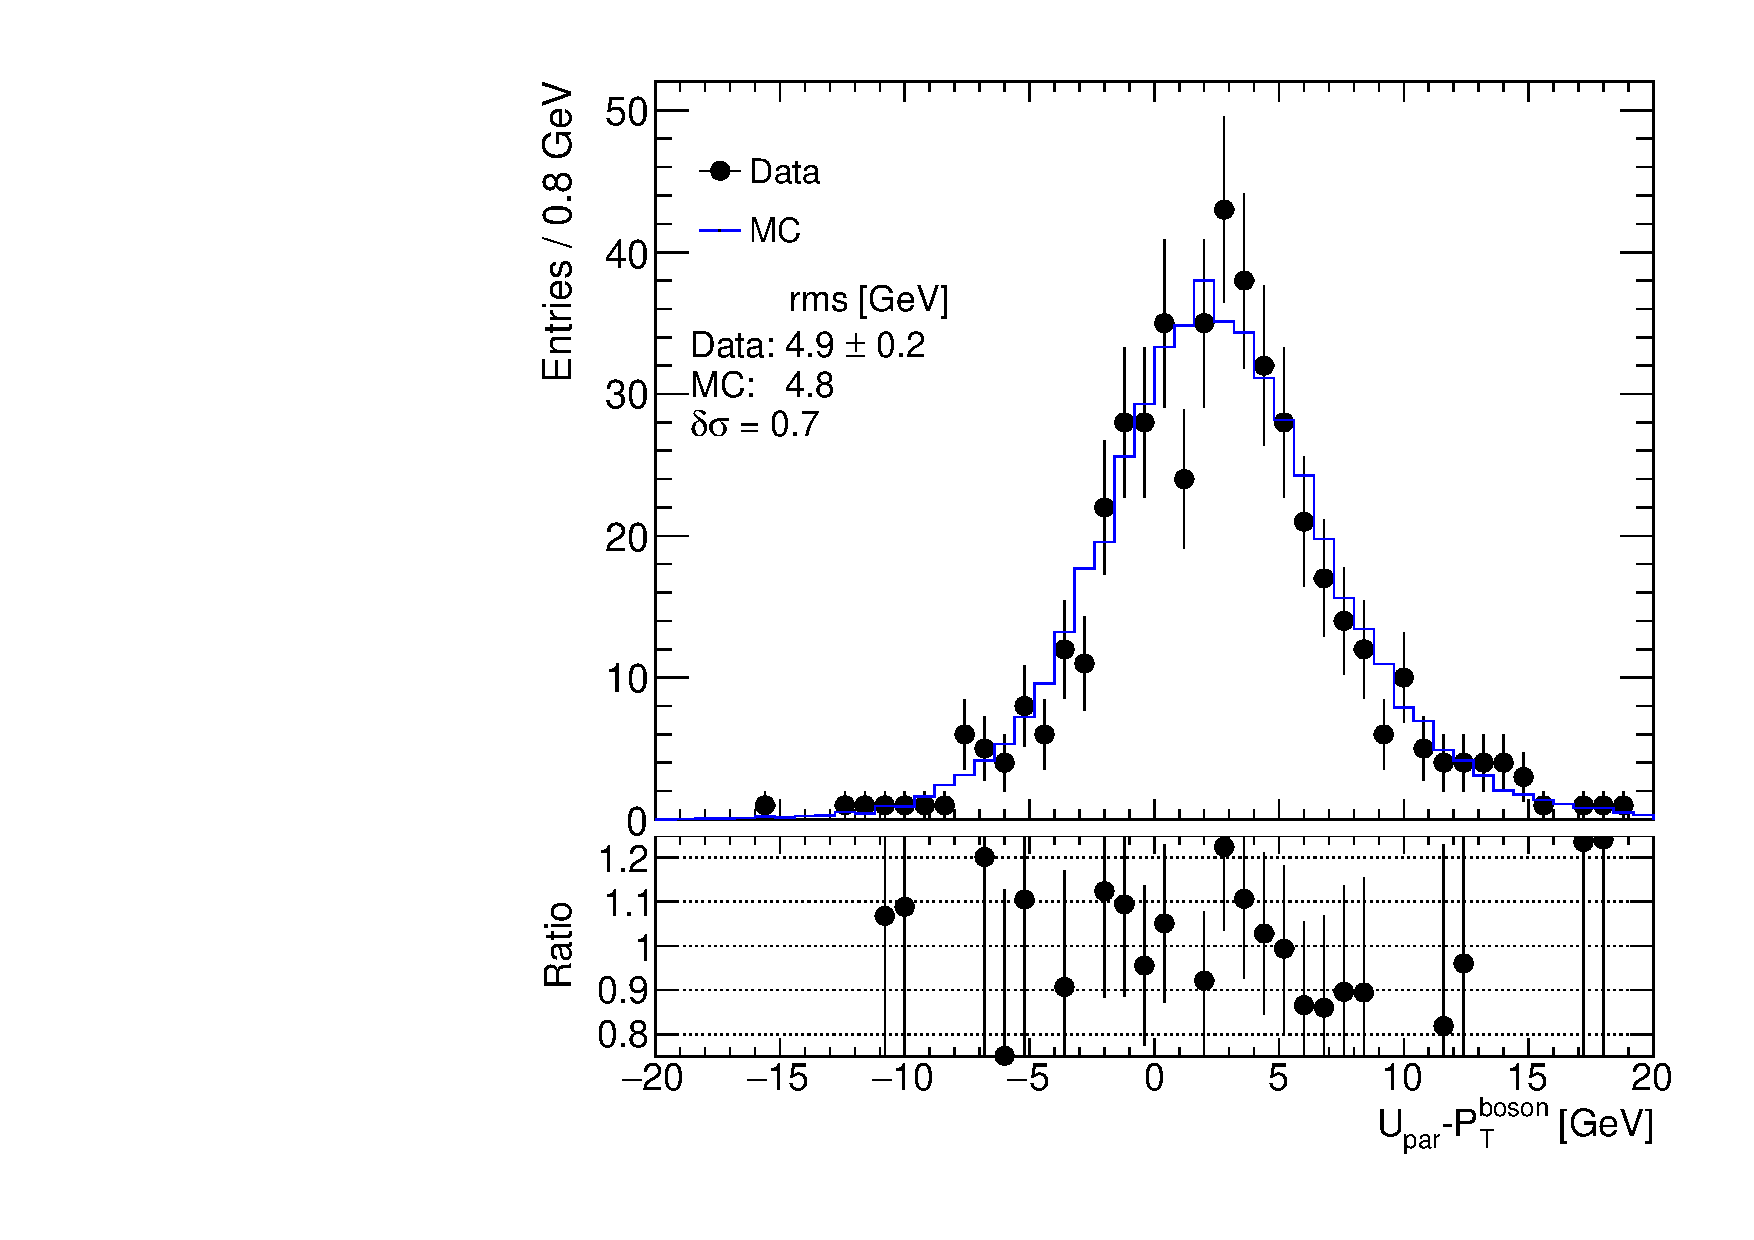
\includegraphics[width=1.\linewidth]{HadronRecoil/UParERMS.pdf} \\ a)}
\end{minipage}
\hfill
\begin{minipage}[h]{0.32\linewidth}
\center{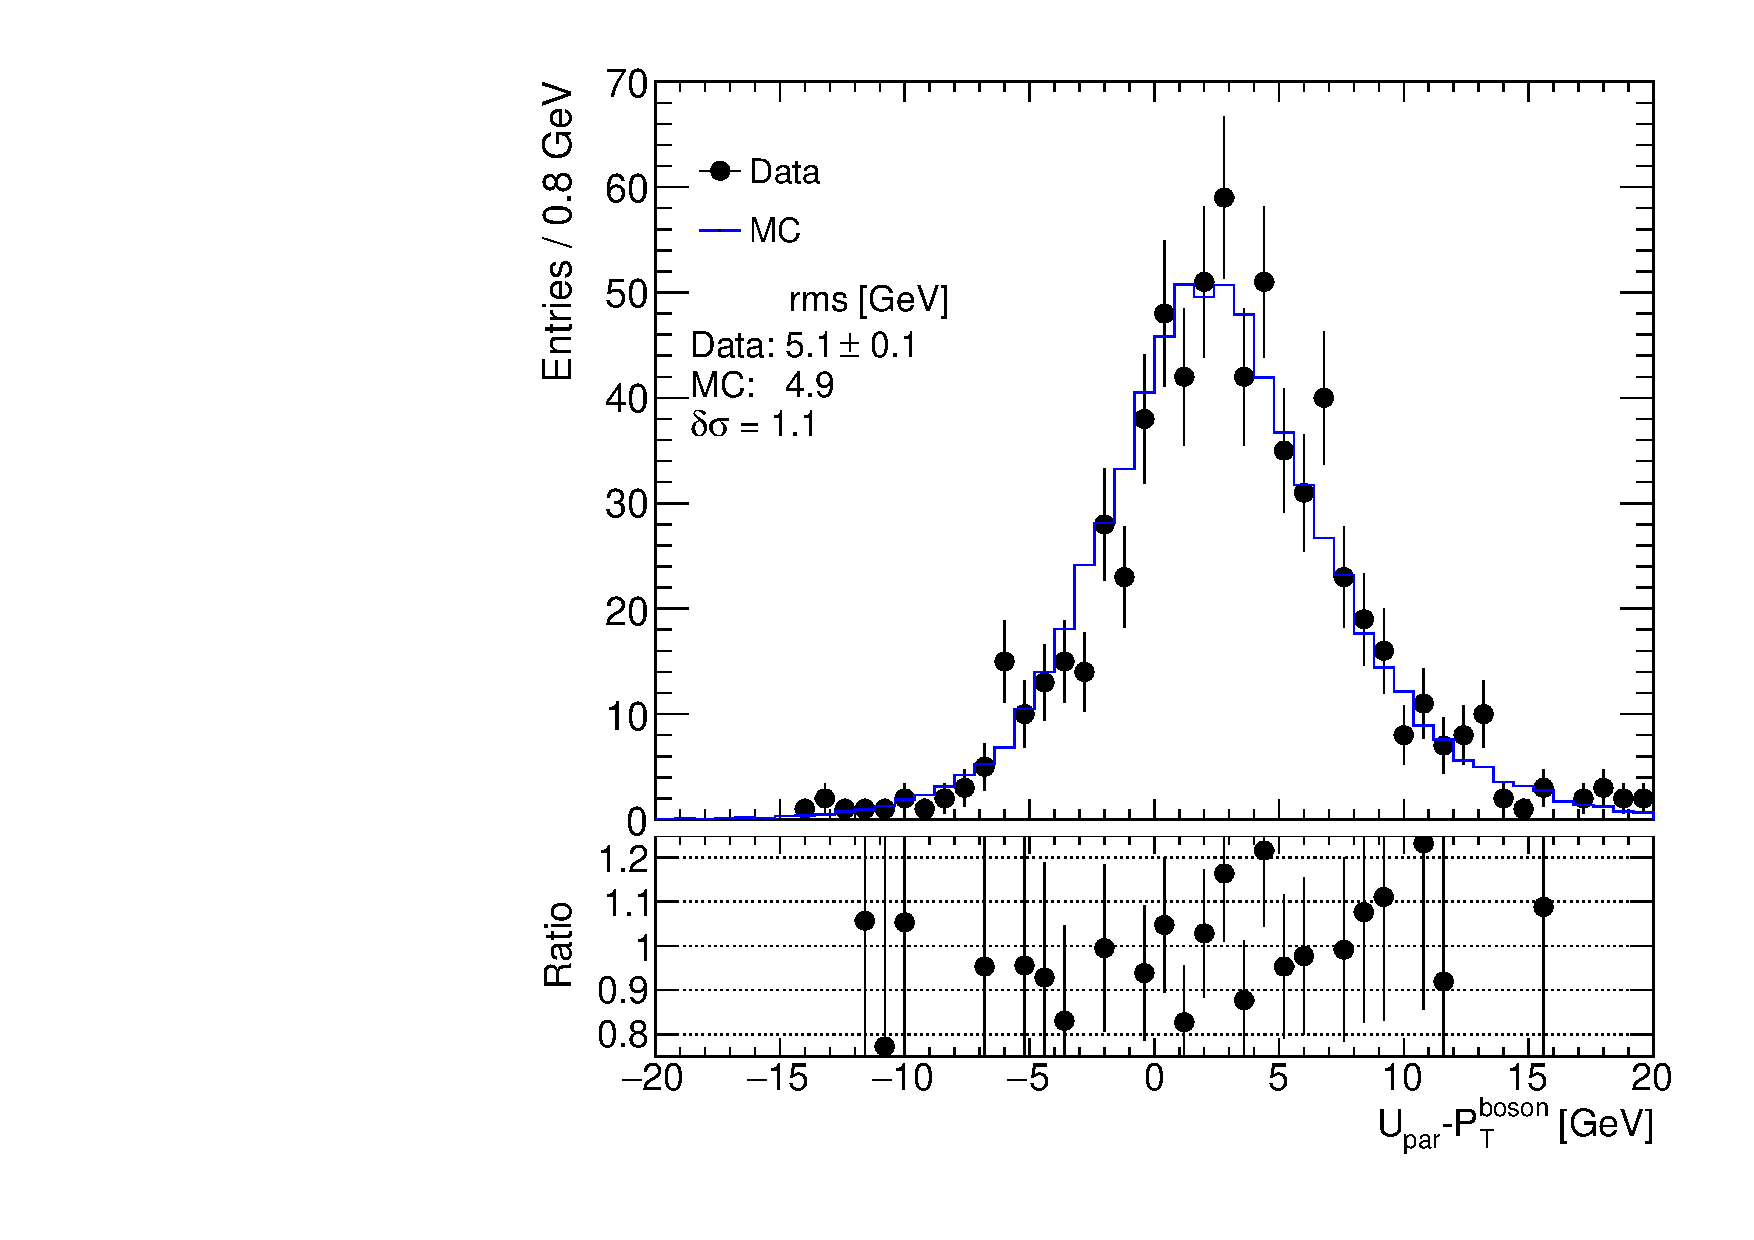
\includegraphics[width=1.\linewidth]{HadronRecoil/UParMRMS.pdf} \\ b)}
\end{minipage}
\hfill
\begin{minipage}[h]{0.32\linewidth}
\center{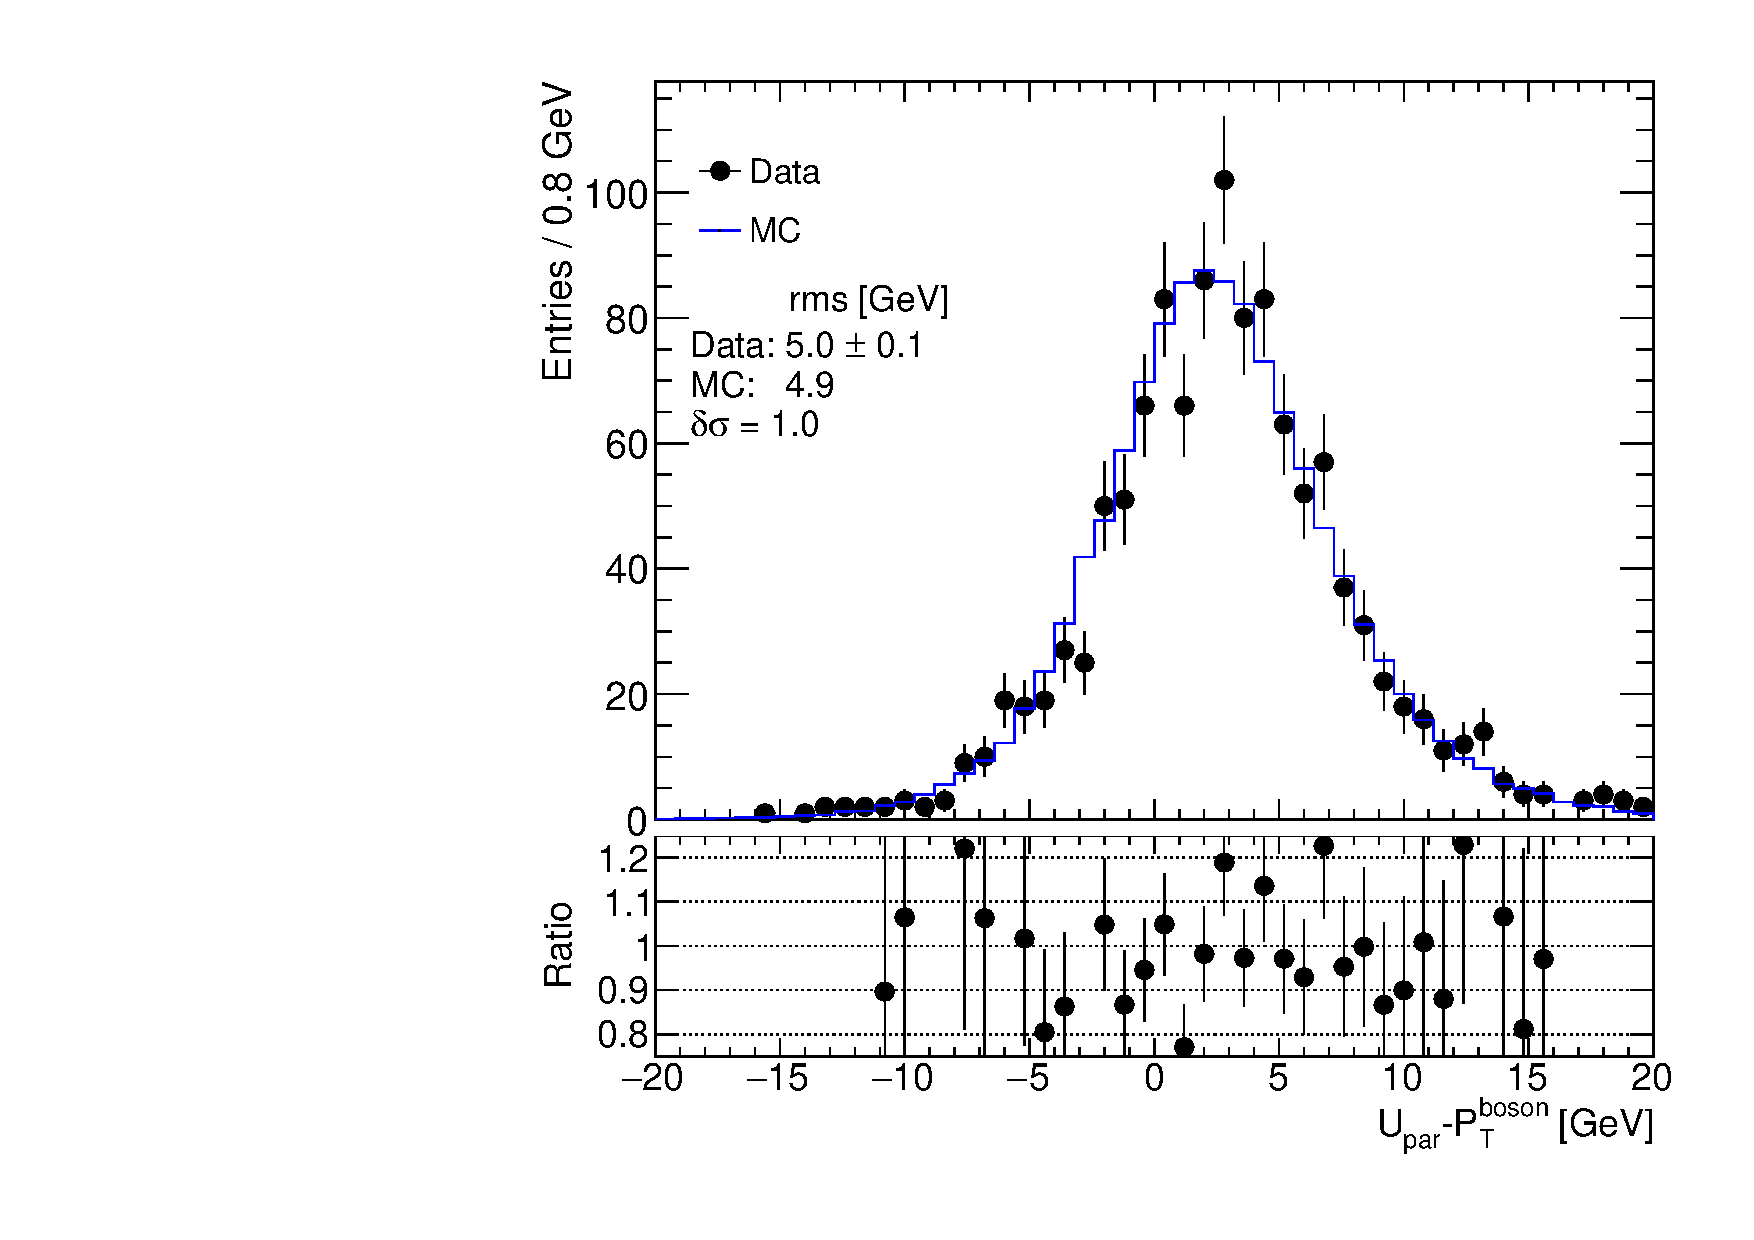
\includegraphics[width=1.\linewidth]{HadronRecoil/UParTotalRMS.pdf} \\ c)}
\end{minipage}
\caption{Difference between parallel hadronic recoil component (\upar) and the transverse momentum of the Z-boson from a) the $Z\to ee$  b) $Z\to\mu\mu$  and c) combined analysis channels. The expected contribution from signal is estimated with Monte Carlo simulation, whereas any background sources are considered negligible.}
\label{HadrRecoil:UparSmear}
\end{figure}

\begin{figure}[!tbp]
\begin{minipage}[h]{0.32\linewidth}
\center{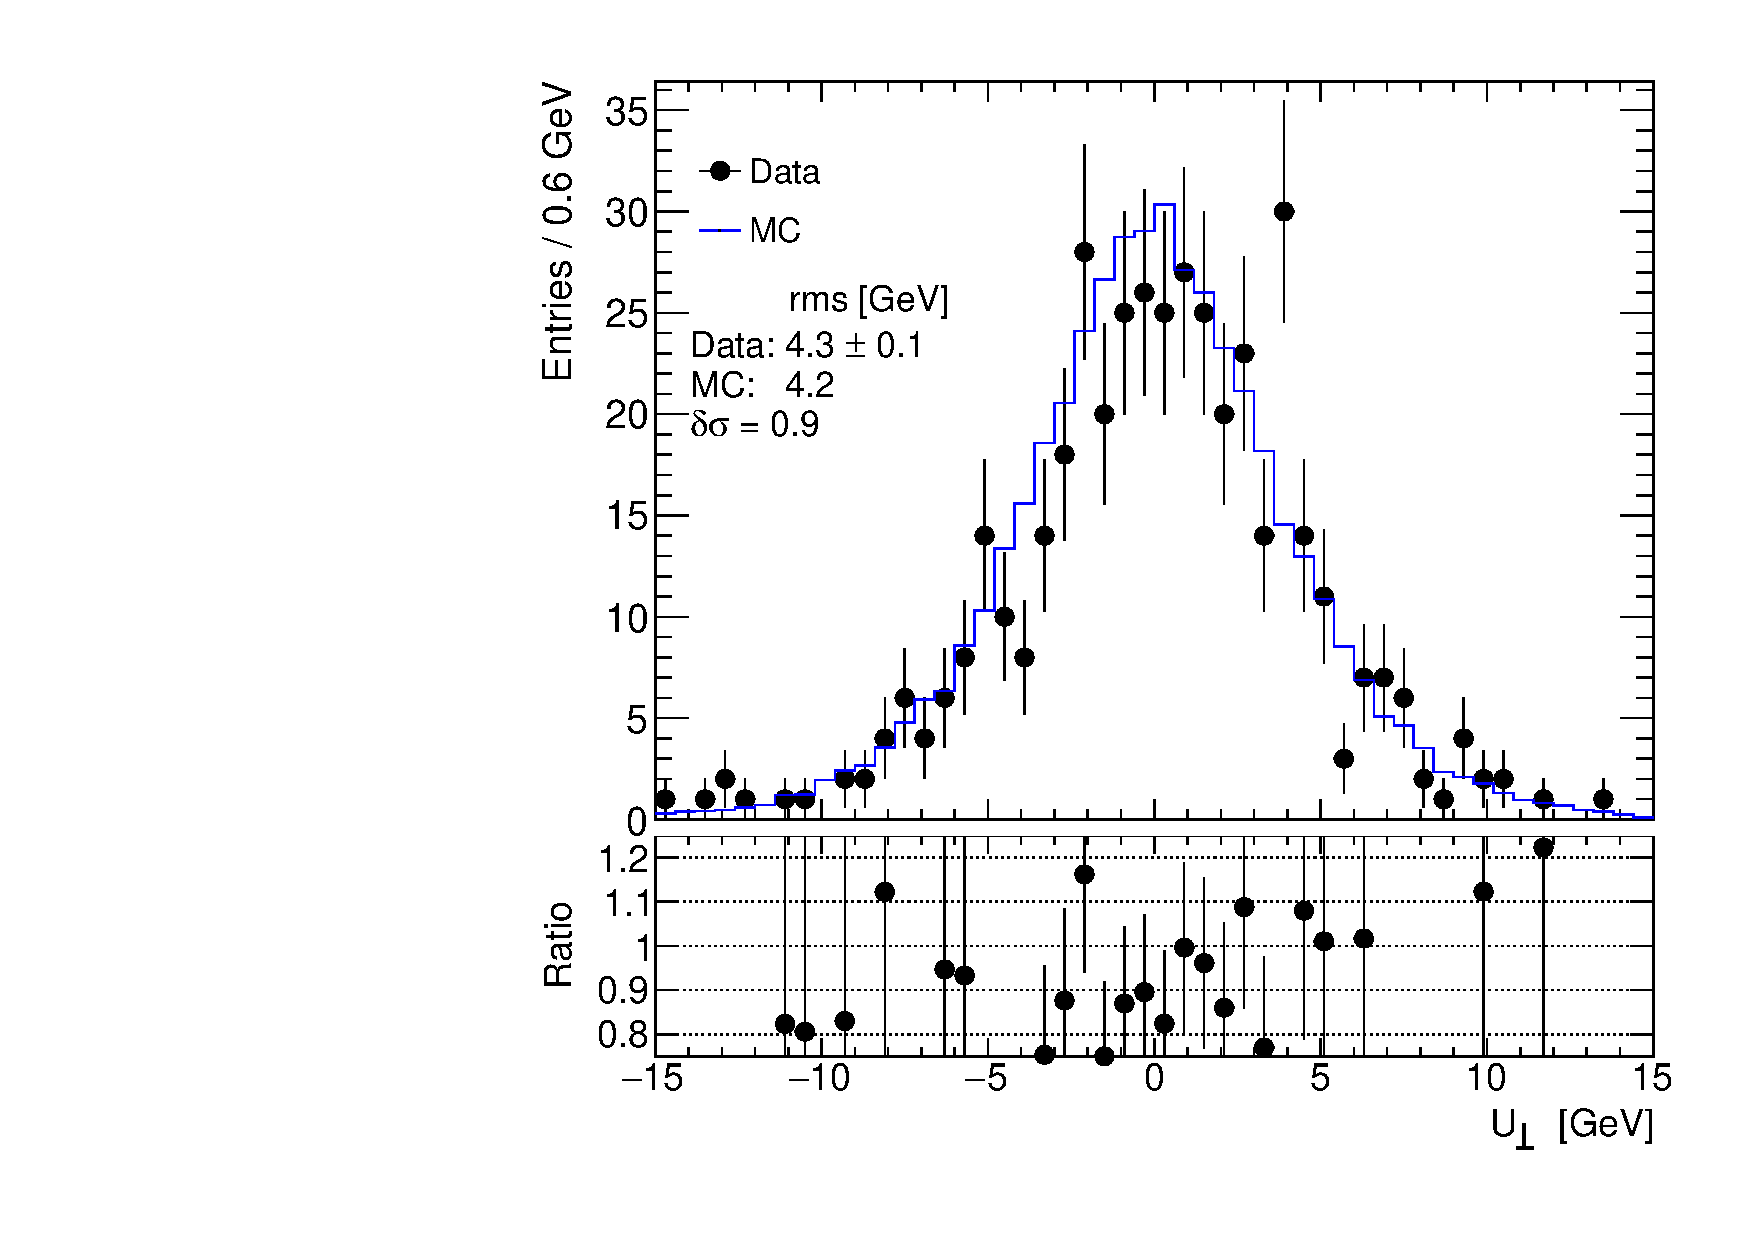
\includegraphics[width=1.\linewidth]{HadronRecoil/UPerpERMS.pdf} \\ a)}
\end{minipage}
\hfill
\begin{minipage}[h]{0.32\linewidth}
\center{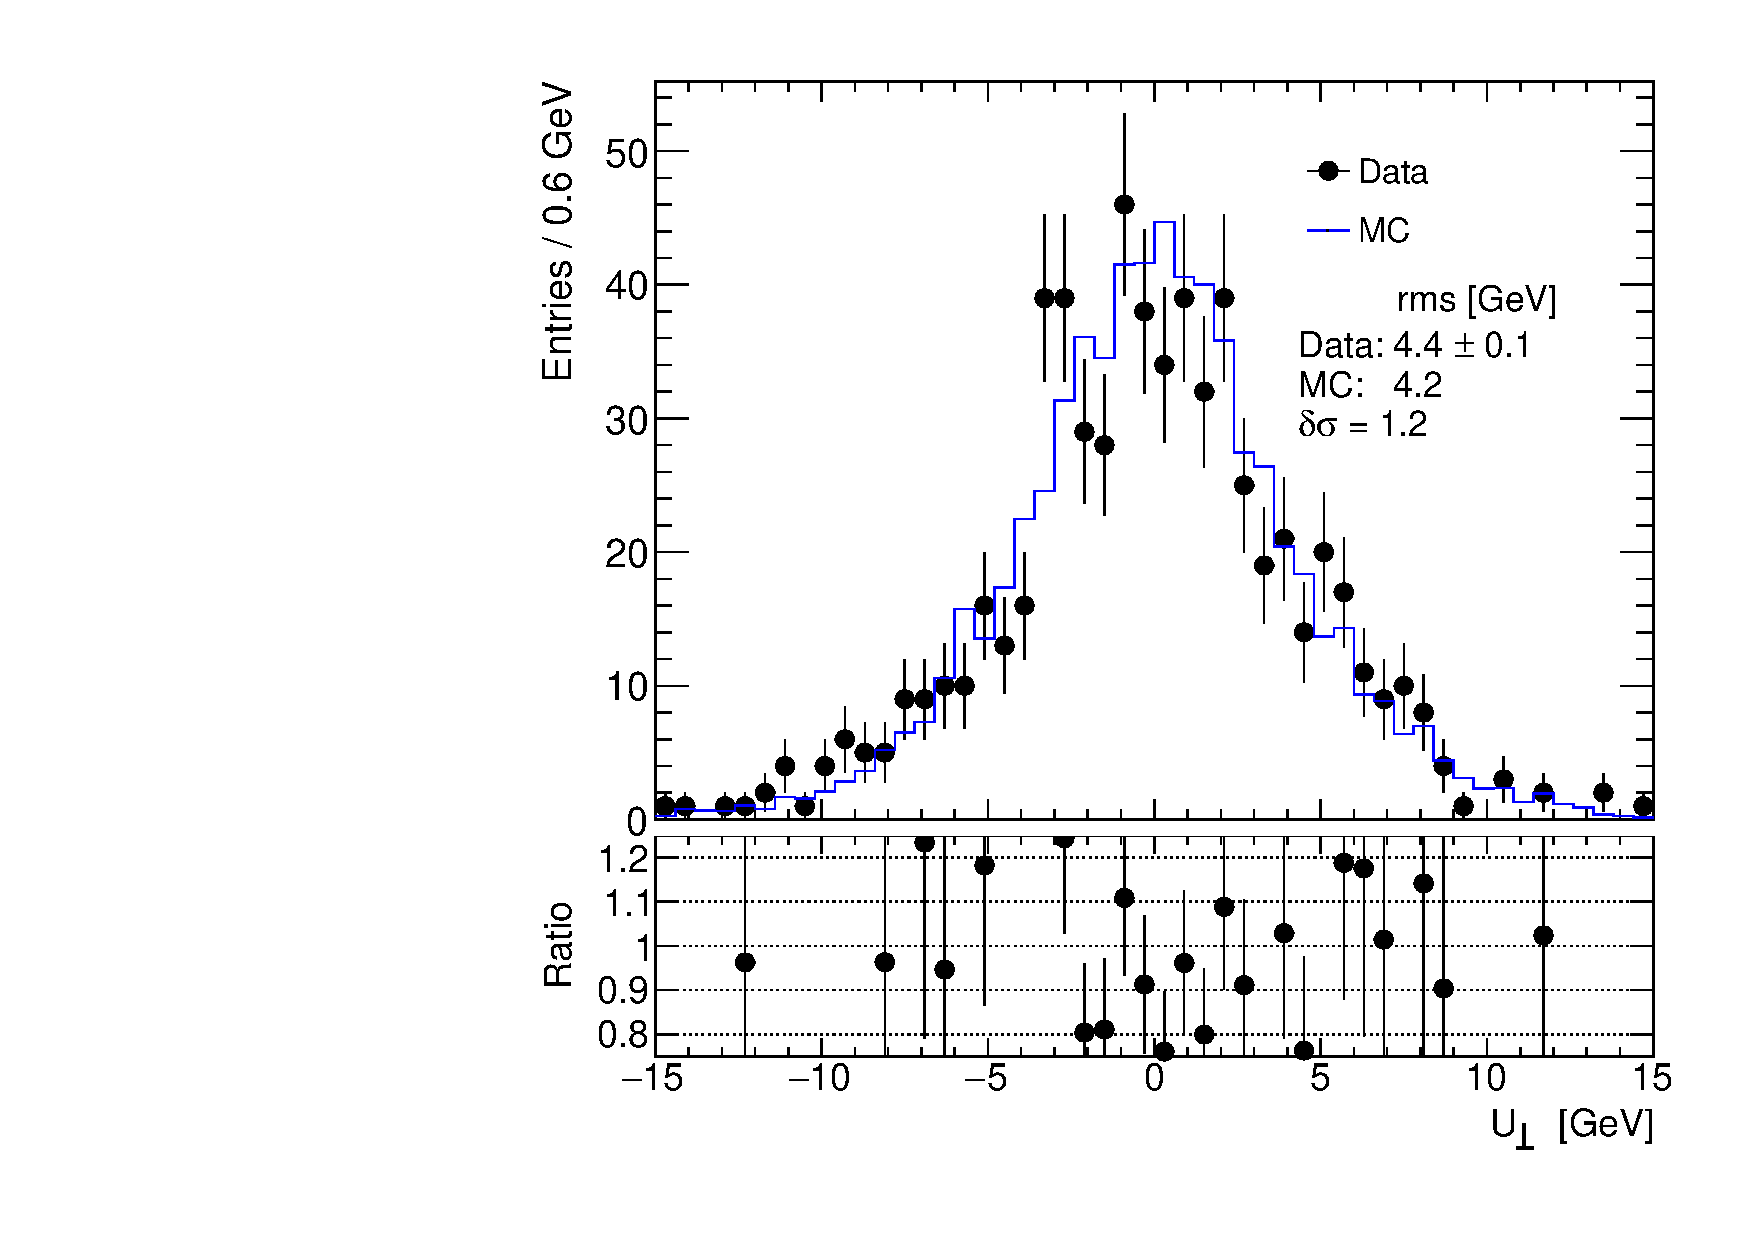
\includegraphics[width=1.\linewidth]{HadronRecoil/UPerpMRMS.pdf} \\ b)}
\end{minipage}
\hfill
\begin{minipage}[h]{0.32\linewidth}
\center{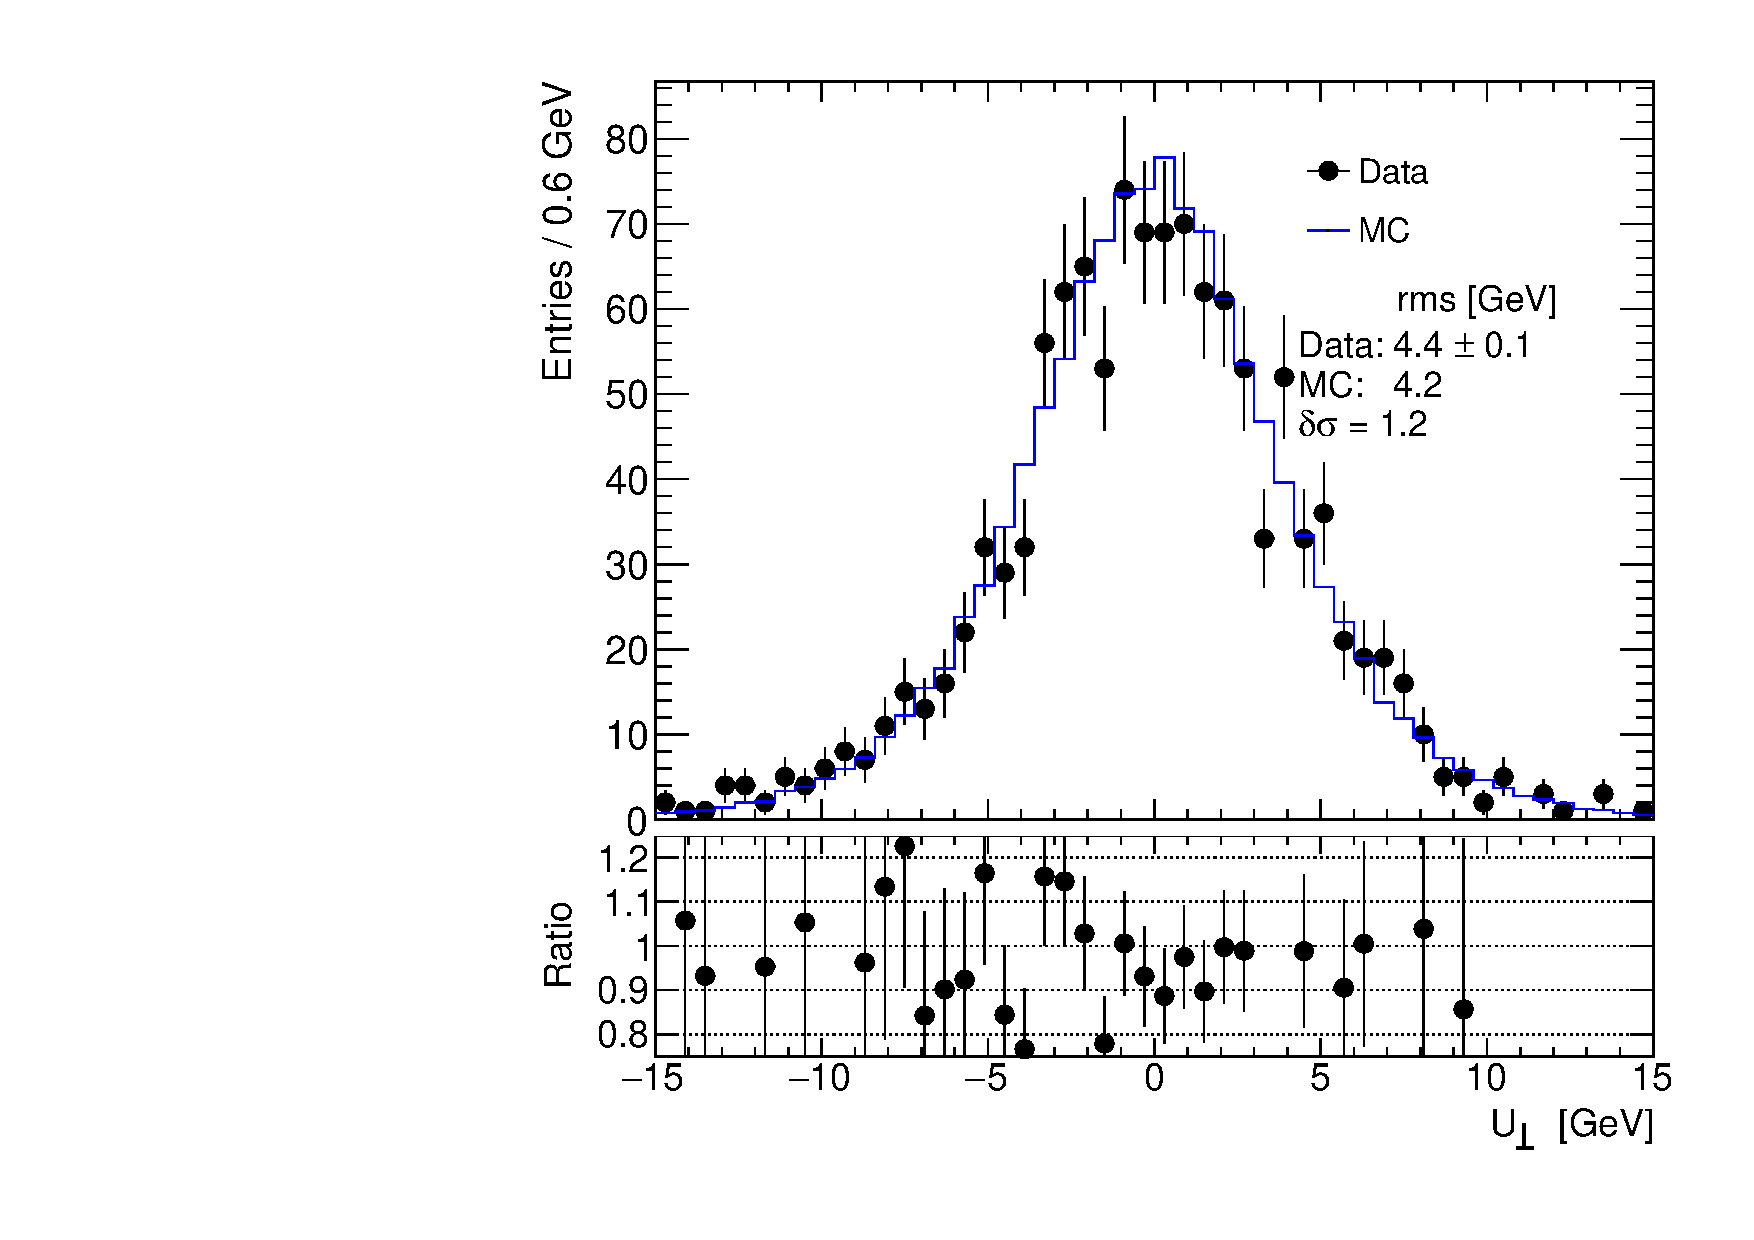
\includegraphics[width=1.\linewidth]{HadronRecoil/UPerpTotalRMS.pdf} \\ c)}
\end{minipage}
\caption{Difference between perpendicular hadronic recoil component (\uperp) and the transverse momentum of the Z-boson from a) the $Z\to ee$  b) $Z\to\mu\mu$  and c) combined analysis channels. The expected contribution from signal is estimated with Monte Carlo simulation, whereas any background sources are considered negligible..}
\label{HadrRecoil:UpeprSmear}
\end{figure}

The hadronic recoil resolution in simulation is corrected using the Gaussian smearing of perpendicular and parallel component of hadronic recoil using the equations:
\begin{equation}
\upar' = \upar+Gaus(0, d\sigma)
\end{equation}
\begin{equation}
\uperp' = \uperp + Gaus(0, d\sigma),
\end{equation}

\subsubsection{Estimation of systematic uncertainty}


The effect of hadronic recoil resolution smearing correction is estimated using On/Off method (Chap.~\ref{chap:Unc}). The scan through the possible $d\sigma$ parameters has shown the decrease of correction factor $C_W$ with the growth of the smearing parameter $d\sigma$. %However, due to the random nature of the correction, the $C_{W}$ fluctuates within the mean value.

The systematic uncertainty is estimated by repeating the correction procedure 25 times (Fig.~\ref{ris:HadrRecSmearStab}). The mean of the obtained parameters $C_{W}$ is treated as a systematic ucertainty of the resolution correction. Tab.~\ref{SmearCW} presents the results of $C_{W}$ systematic error measurement together with standard deviation and the error of the mean, calculated as:
\begin{equation}\label{eq:MeanErr2}
U \Big( C_W \Big) = \frac{\sigma( C_{W} )}{\sqrt N},
\end{equation}
where $\sigma(C_w)$ is a standard deviation of $C_W$ distribution and $N=25$ is a total number of repetitions used. An overall systematic effect is below 0.2\% for each analysis channel, what is significantly lower than a statistical uncertainty for the W-boson analyses (Chap.~\ref{chap:Unc}).

\begin{figure}[!tbp]
\begin{minipage}[h]{0.49\linewidth}
\center{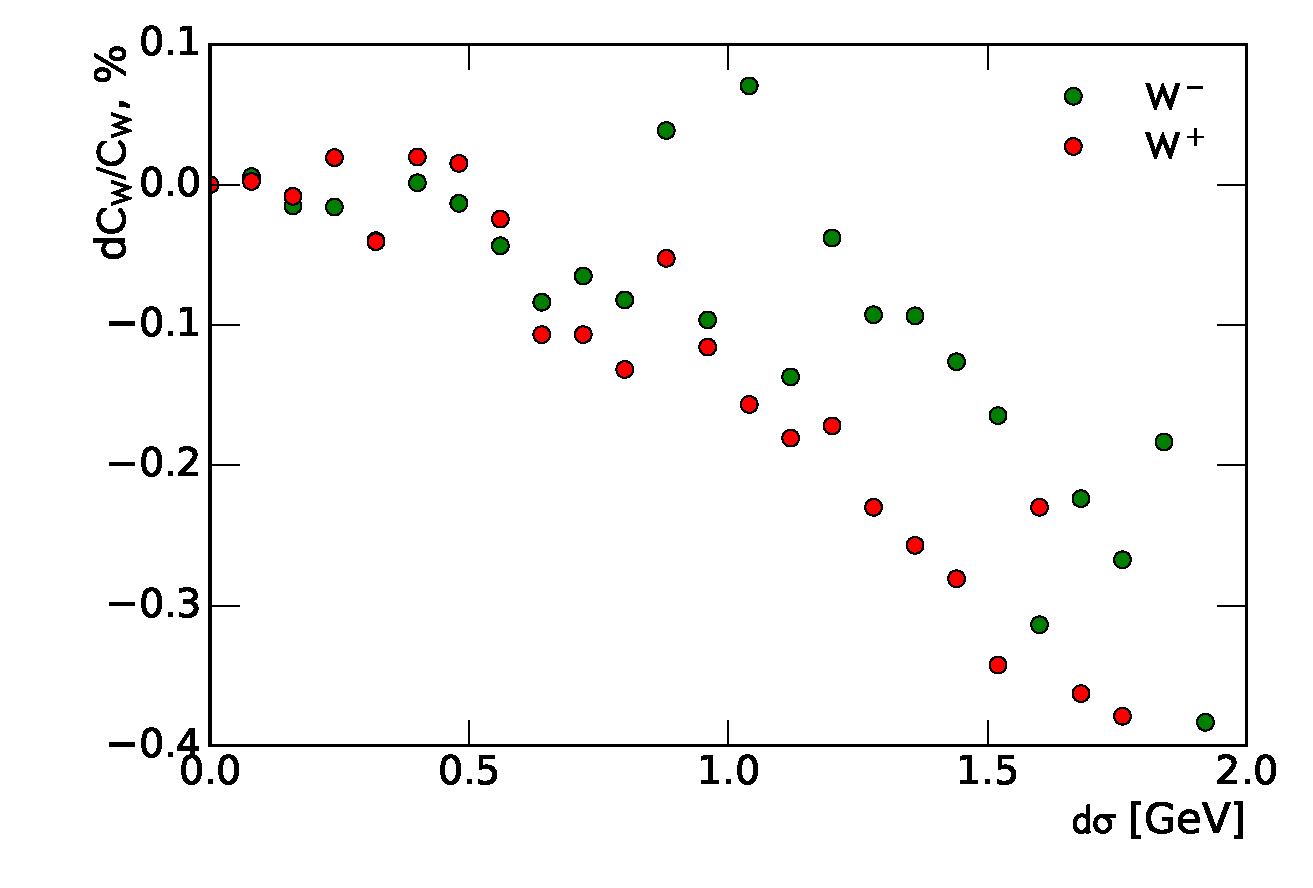
\includegraphics[width=1.\linewidth]{HadronRecoil/CWElectronSmearing.pdf} \\ a)}
\end{minipage}
\hfill
\begin{minipage}[h]{0.49\linewidth}
\center{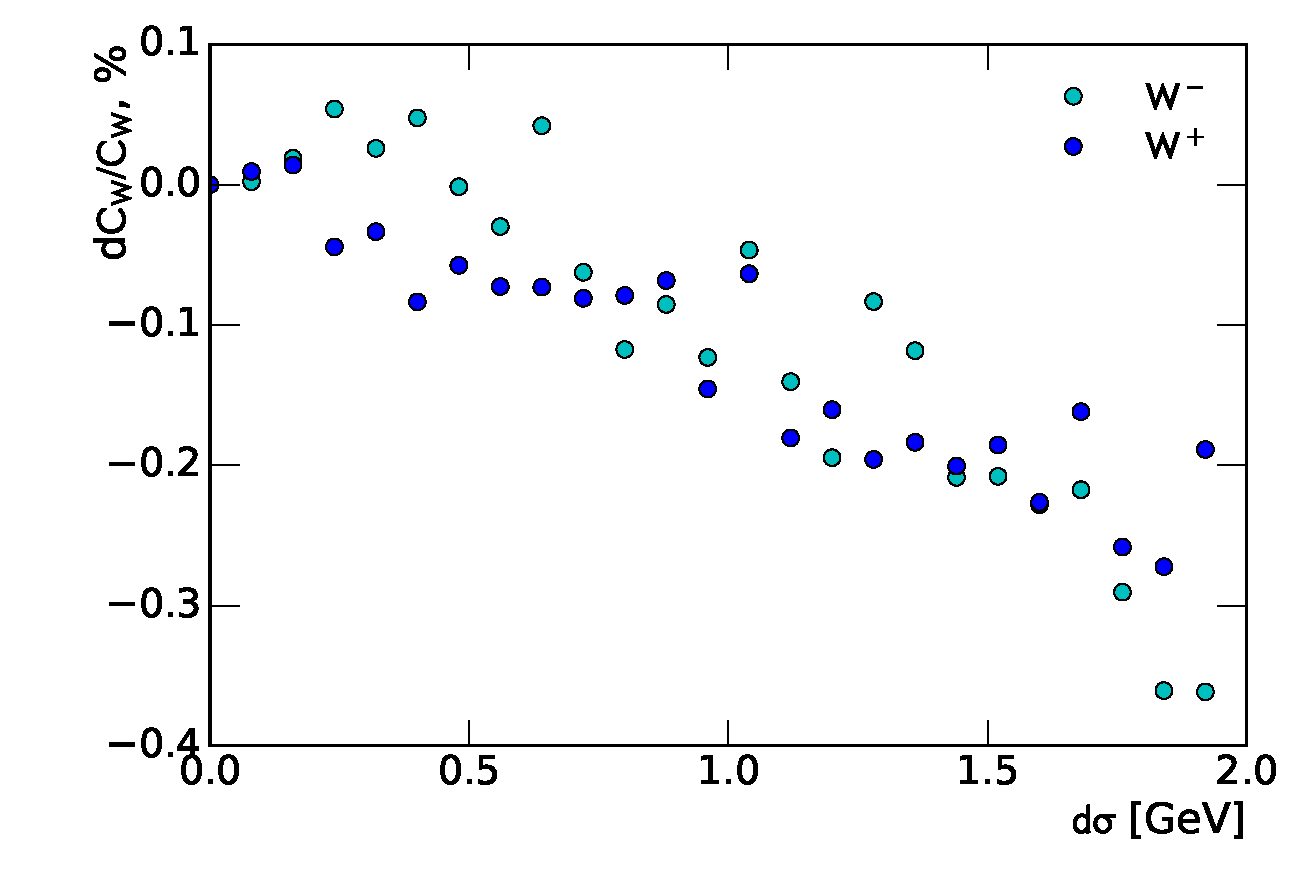
\includegraphics[width=1.\linewidth]{HadronRecoil/CWMuonSmearing.pdf} \\ b)}
\end{minipage}
\caption{Shift in correction factor \cw from hadronic recoil resolution correction as a a function of smearing correction ($d\sigma$) for a) \wenu b) \wmunu analysis channels.}
\label{ris:HadrRecSmearScan}
\end{figure}

\begin{figure}[!tbp]
\begin{minipage}[h]{0.49\linewidth}
\center{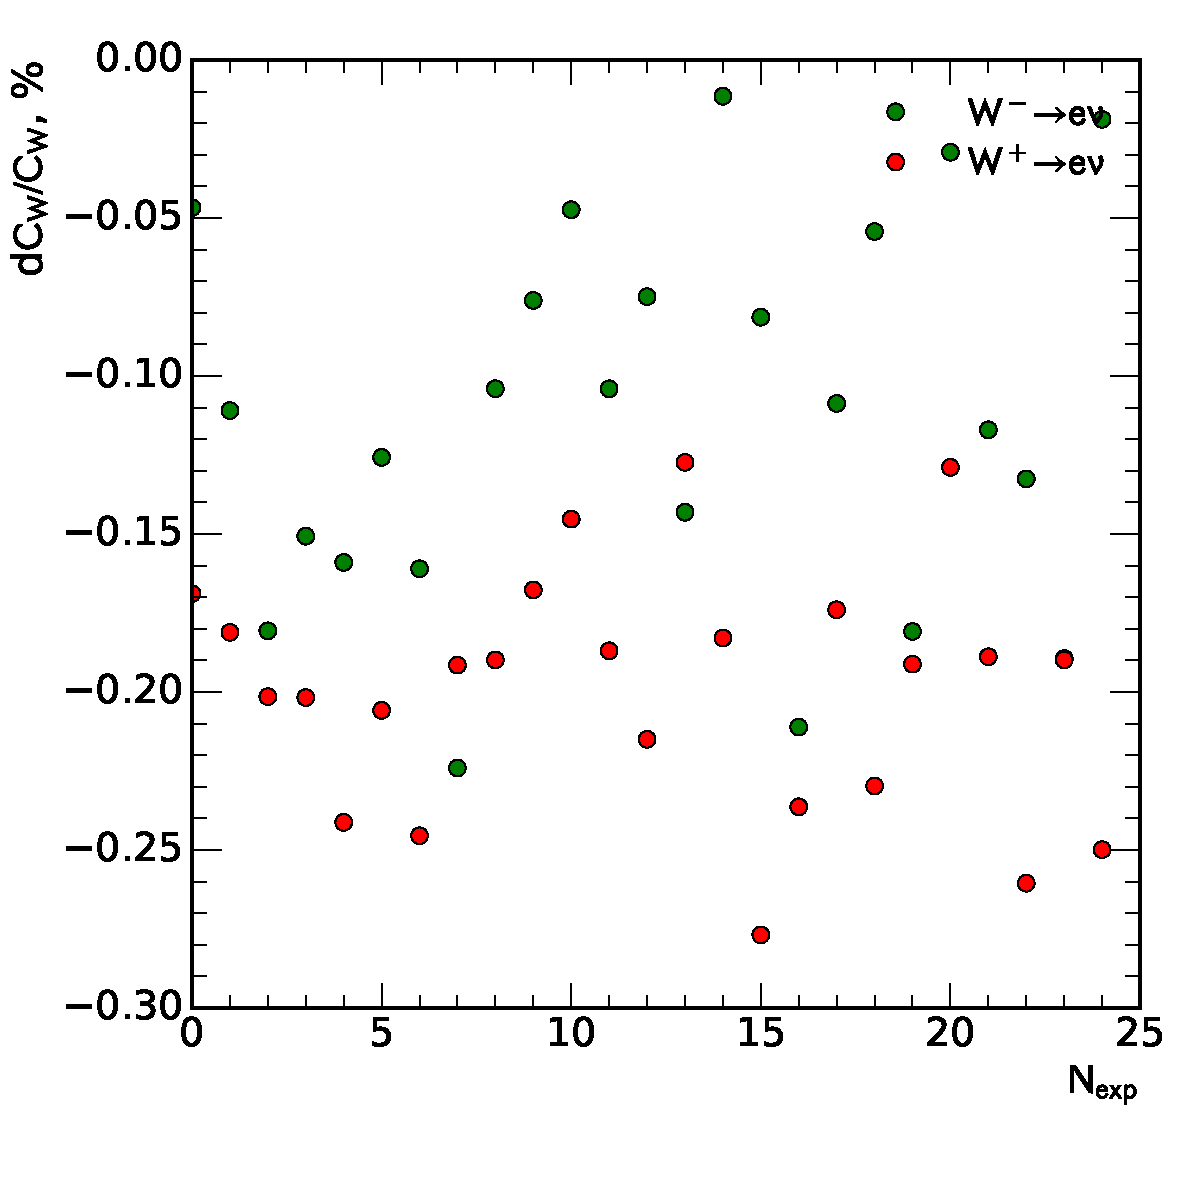
\includegraphics[width=1.\linewidth]{HadronRecoil/CWElectronStab.pdf} \\ a)}
\end{minipage}
\hfill
\begin{minipage}[h]{0.49\linewidth}
\center{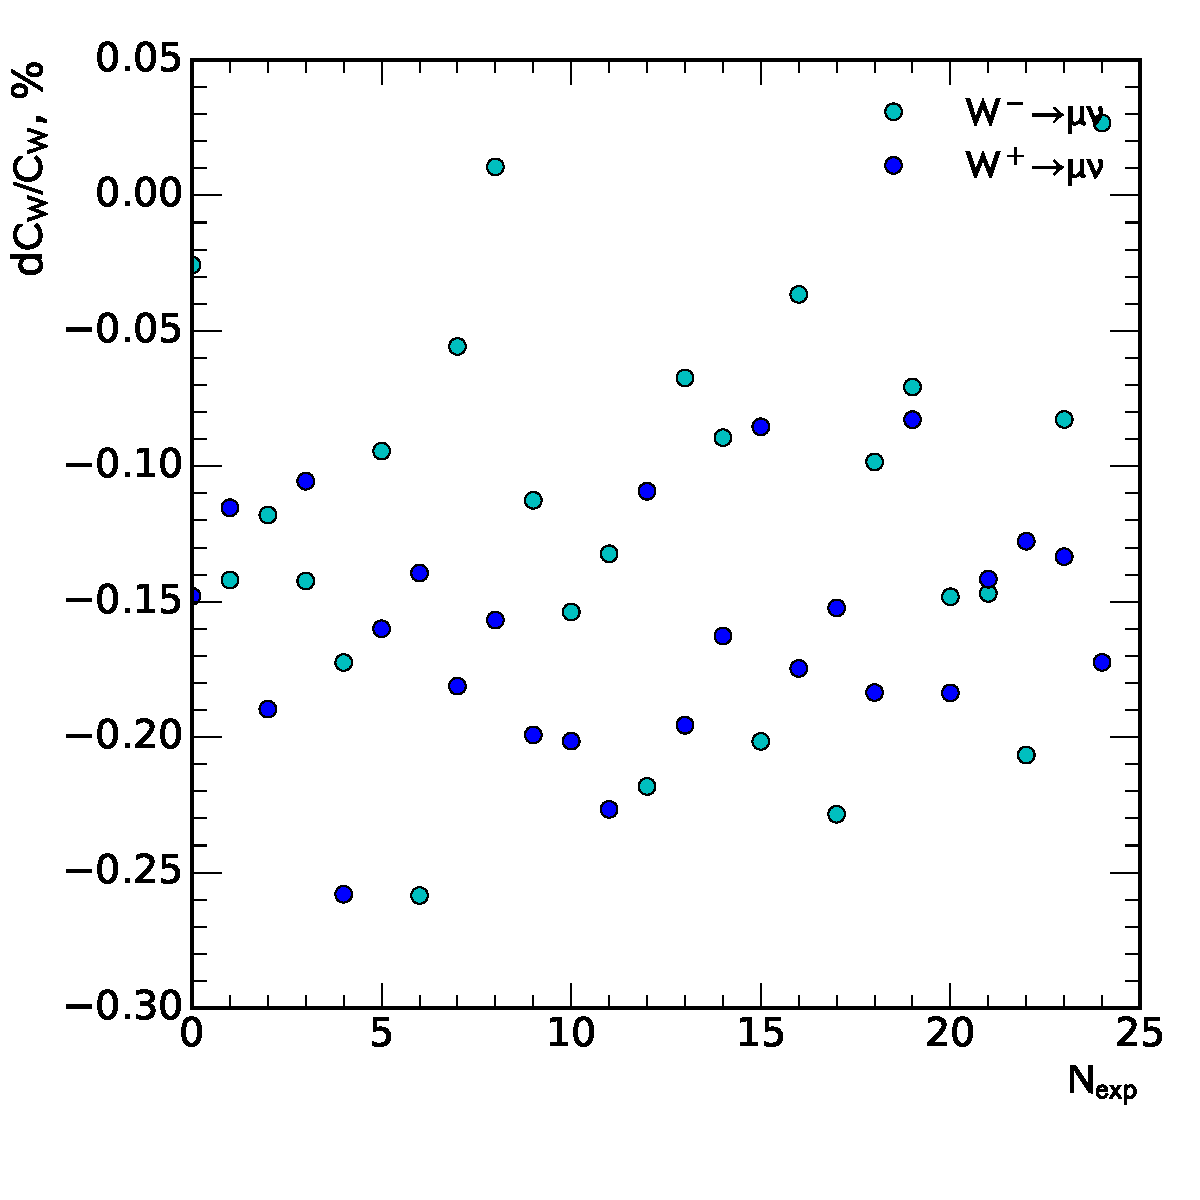
\includegraphics[width=1.\linewidth]{HadronRecoil/CWMuonStab.pdf} \\ b)}
\end{minipage}
\caption{Shift in correction factor \cw from hadronic recoil resolution correction ($d\sigma$ = 1.3 GeV) for a) \wenu b) \wmunu analysis channels as a function of number of repetitions.}
\label{ris:HadrRecSmearStab}
\end{figure}


 \begin{table}[!t]
 \caption{The effect of hadronic recoil smearing correction on $C_{W}$ for different channels. The statistical error (noted $stat.err.$) of the mean value is estimated using Eq.~\ref{eq:MeanErr2}.}
\label{SmearCW}
\begin{center}
\begin{tabular}{| l  | c | c | }
\hline
Channel & $\delta C_W \pm stat.\, err.$ & rms \\
\hline
\hline
$W^{+} \to e^{+}\nu$ & -0.20$\pm0.01$\% & 0.04\% \\
$W^{-} \to e^{-}\nu$ & -0.11$\pm0.01$\% &  0.06\% \\
\hline
$W^{+} \to \mu^{+}\nu$ & -0.16$\pm0.01$\% & 0.04\% \\
$W^{-} \to \mu^{-}\nu$ & -0.12$\pm0.01$\% & 0.07\% \\
\hline
\end{tabular}
\end{center}

\end{table}

\section{Hadronic recoil bias correction}\label{sec:HRBias}


As it was mentioned in Sec,~\ref{sec:HRIntro}, the hadronic recoil distribution in the simulation may be shifted with respect to the data due to the mismodelling of the underlying event and calorimeter cluster responses. The correction of the hadronic recoil bias is performed by applying the relevant correction factor $HR_{SF}$ on a hadronic recoil in simulation:
\begin{equation}
\upar^{cor}=\upar \cdot HR_{SF},
\end{equation}
where \upar is the parallel component of the hadronic recoil measured with the respect to the W-boson direction.

\begin{figure}[!b]
\minipage{0.32\textwidth}
  \center{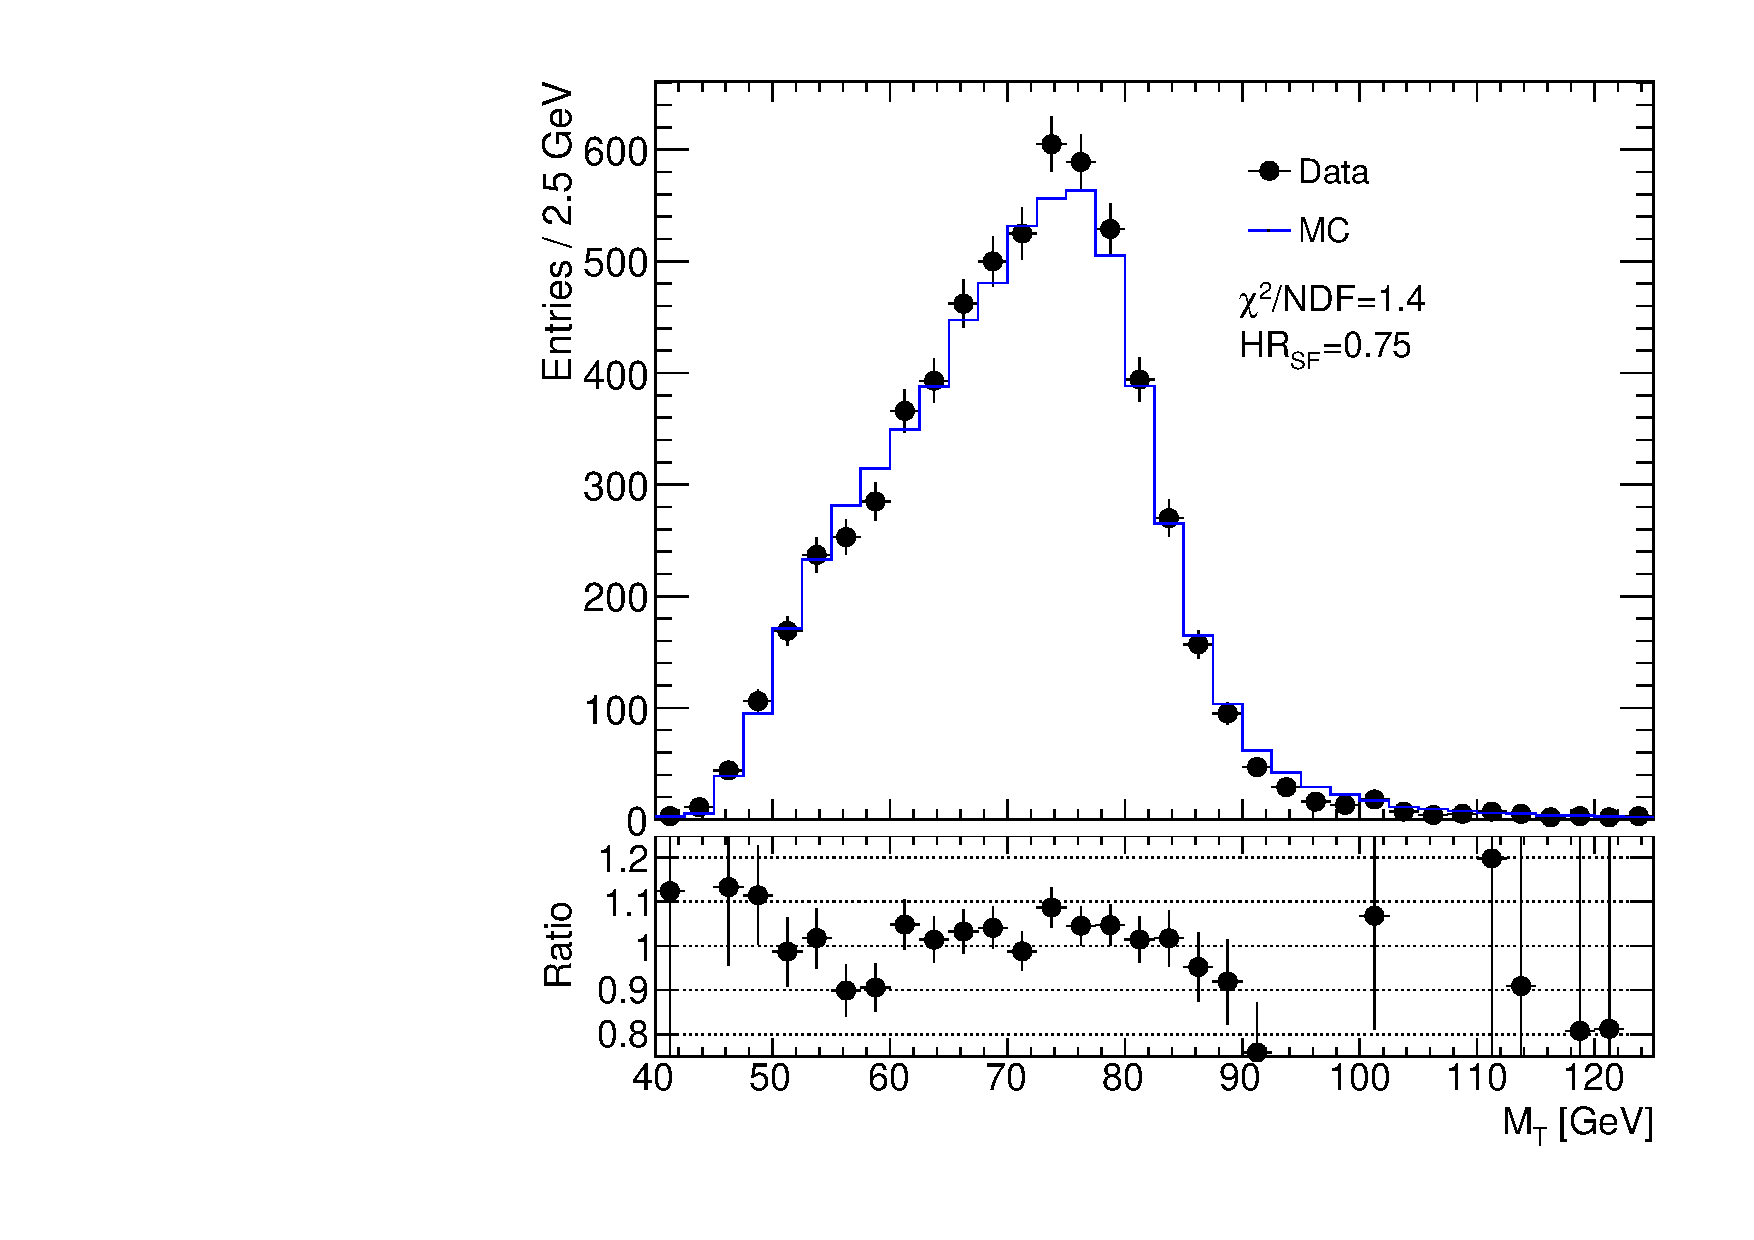
\includegraphics[width=\linewidth]{HadronRecoil/MtWEScale0.pdf} a)}
\endminipage\hfill
\minipage{0.32\textwidth}
   \center{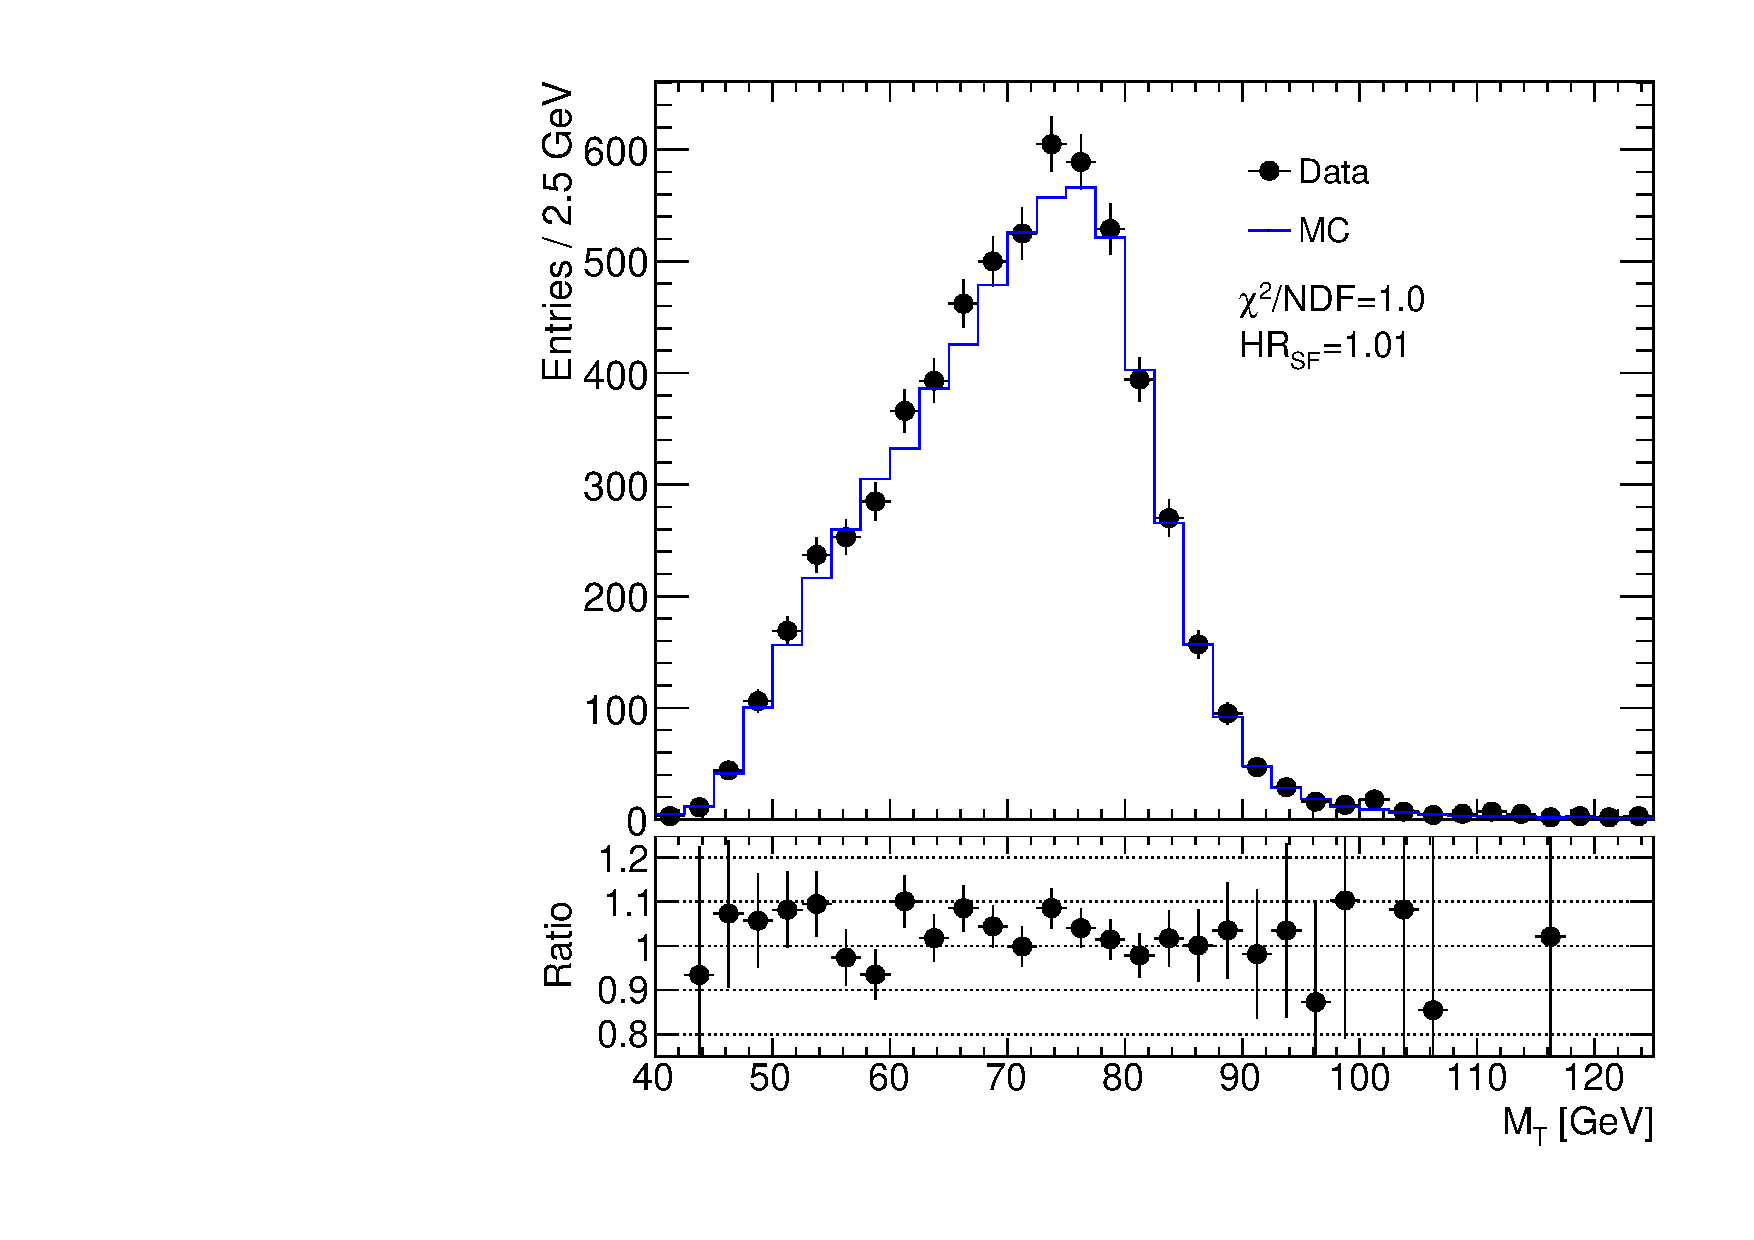
\includegraphics[width=\linewidth]{HadronRecoil/MtWEScale13.pdf} b)}
\endminipage\hfill
\minipage{0.32\textwidth}%
   \center{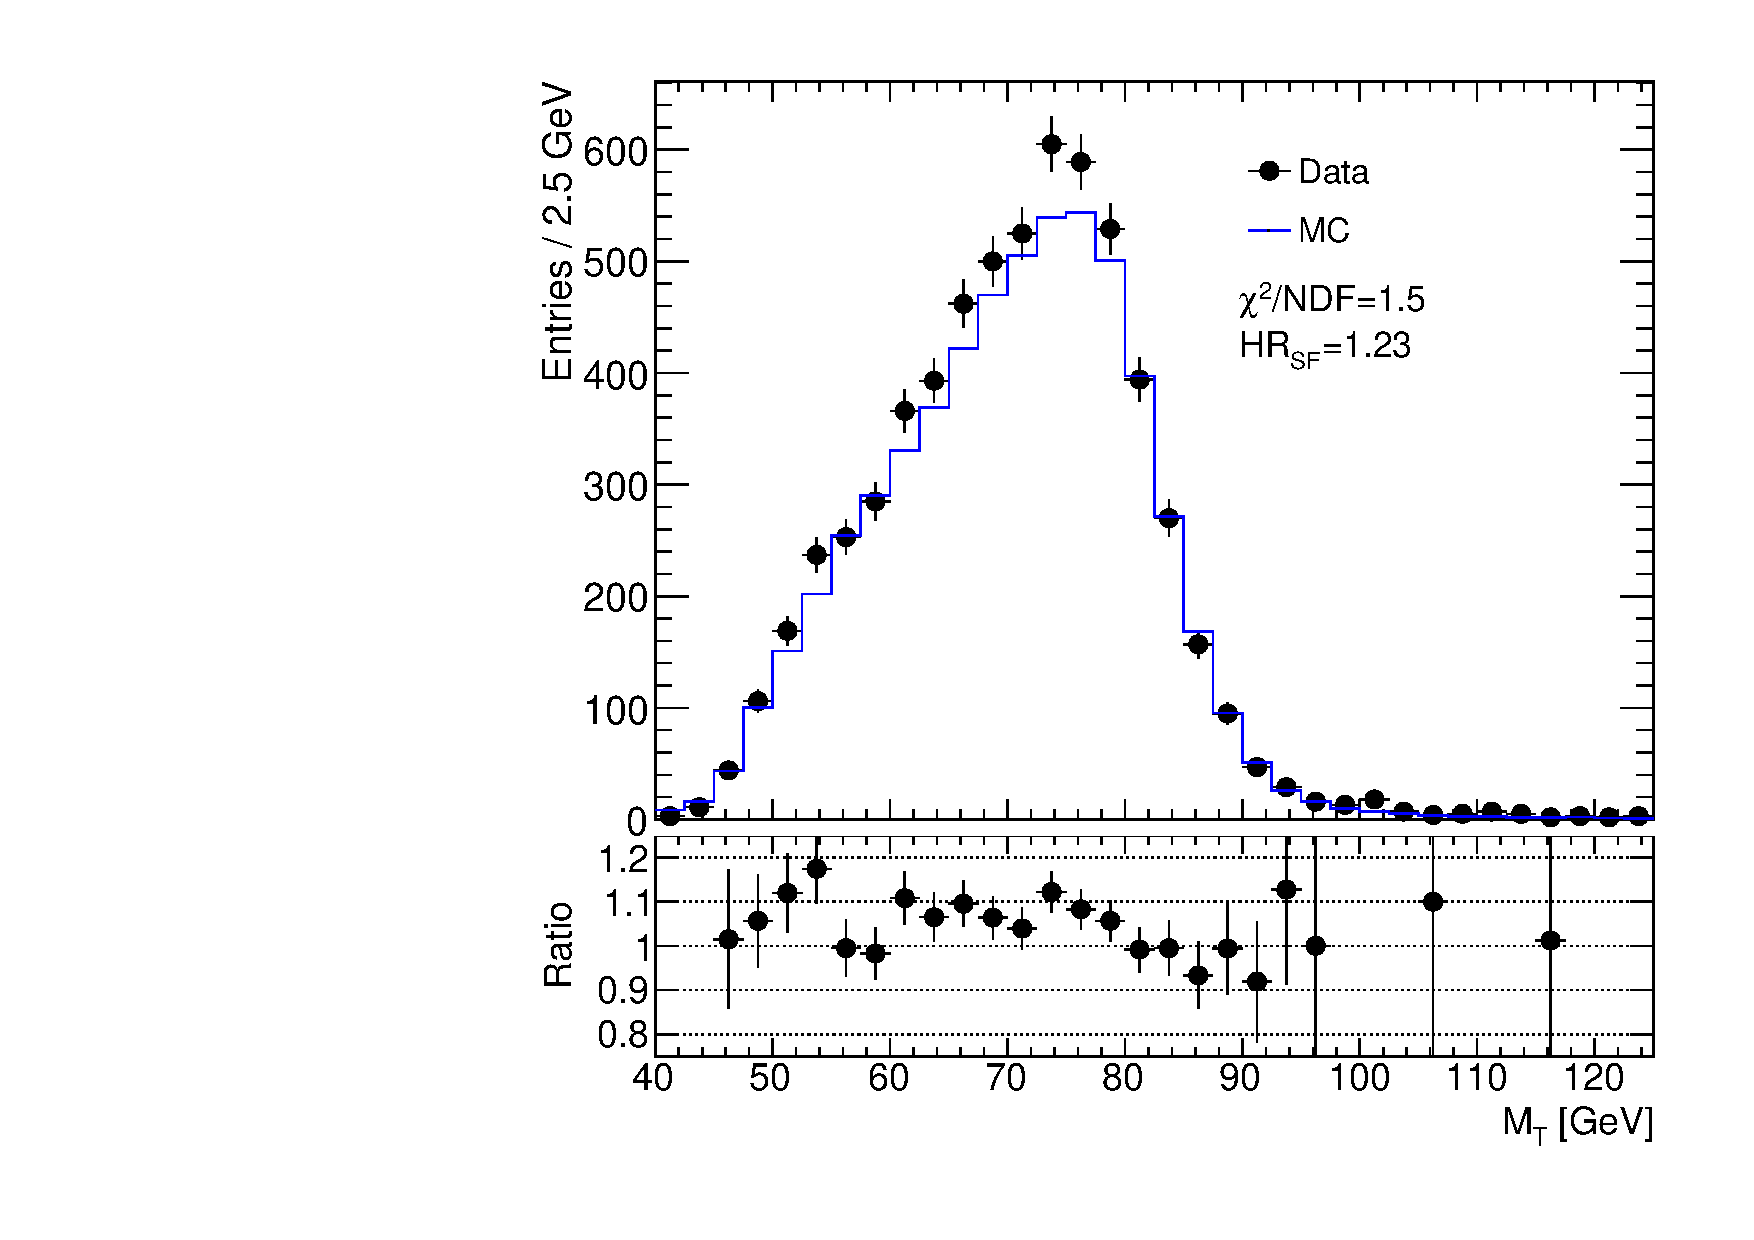
\includegraphics[width=\linewidth]{HadronRecoil/MtWEScale24.pdf} c)}
\endminipage
\caption{Transverse mass distribution for the \wenu event candidates for different  choice of hadronic recoil correction factors: a) $HR_{SF}$=0.75 b) $HR_{SF}$= 1.1 c) $HR_{SF}$=1.23. The expected contributions from signal and background processes are estimated using Monte Carlo simulation.}
\label{HadronRecoilScaleMtW}
\end{figure}

The determination of the optimal parameter $HR_{SF}$ is performed through the scan of correction factor values. It is assumed that the best value of the hadronic recoil bias corresponds to the best agreement between the data and simulation, tested using the $\chiD$-test. The correction value is obtained through the \chiD fit of \chiD-test results using the to the function:
\begin{equation}\label{eq:chiD}
\chi^2 = \frac{(HR_{SF}-sf_{best})^2}{\sigma_{sf}^2}+\chi^2_0,
\end{equation}
where $sf_{best}$ is the hadronic recoil correction scale factor, obtained from the \chiD fit,  $\sigma_{sf}$ is a statistical error of correction factor and $\chi^2_0$ is a value of \chiD in its minimum. 

In the following sections methods of hadronic recoil bias determination using W and Z-boson candidate events are discussed.

\subsection{Bias determination from the \mtw distribution}


The hadronic recoil bias determination is performed using the distributions, that  are not sensitive to the true \ptw spectrum, to exclude the effect of possible \ptw mismodelling in the simulation.  One of the optimal choices is the \mtw distribution. Transverse mass distribution for different values of correction factors $HR_{SF}$ is shown in Fig.~\ref{HadronRecoilScaleMtW}. 

\begin{figure}[!tbp]
\begin{minipage}[h]{0.49\linewidth}
\center{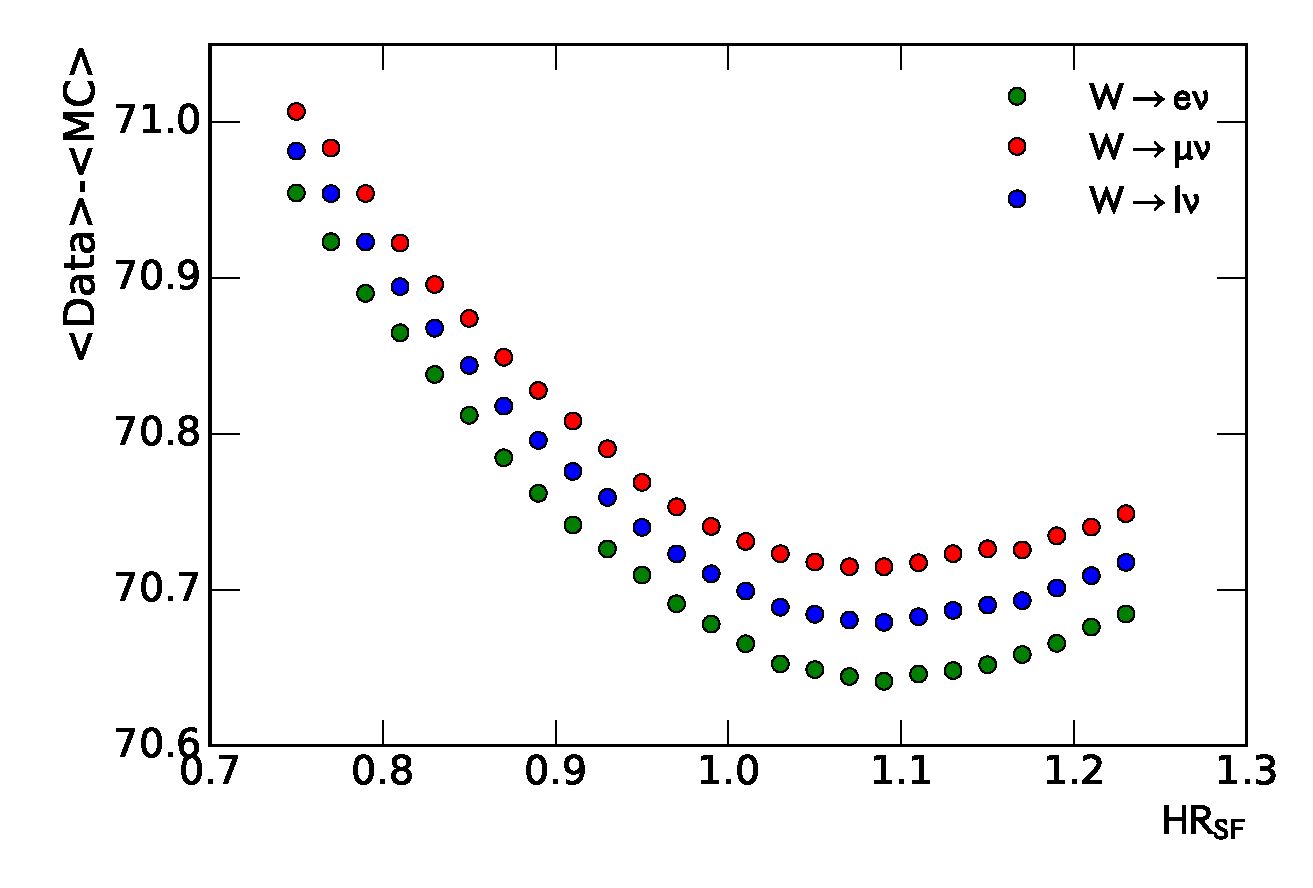
\includegraphics[width=1.\linewidth]{HadronRecoil/MeanAll.pdf} \\ a)}
\end{minipage}
\hfill
\begin{minipage}[h]{0.49\linewidth}
\center{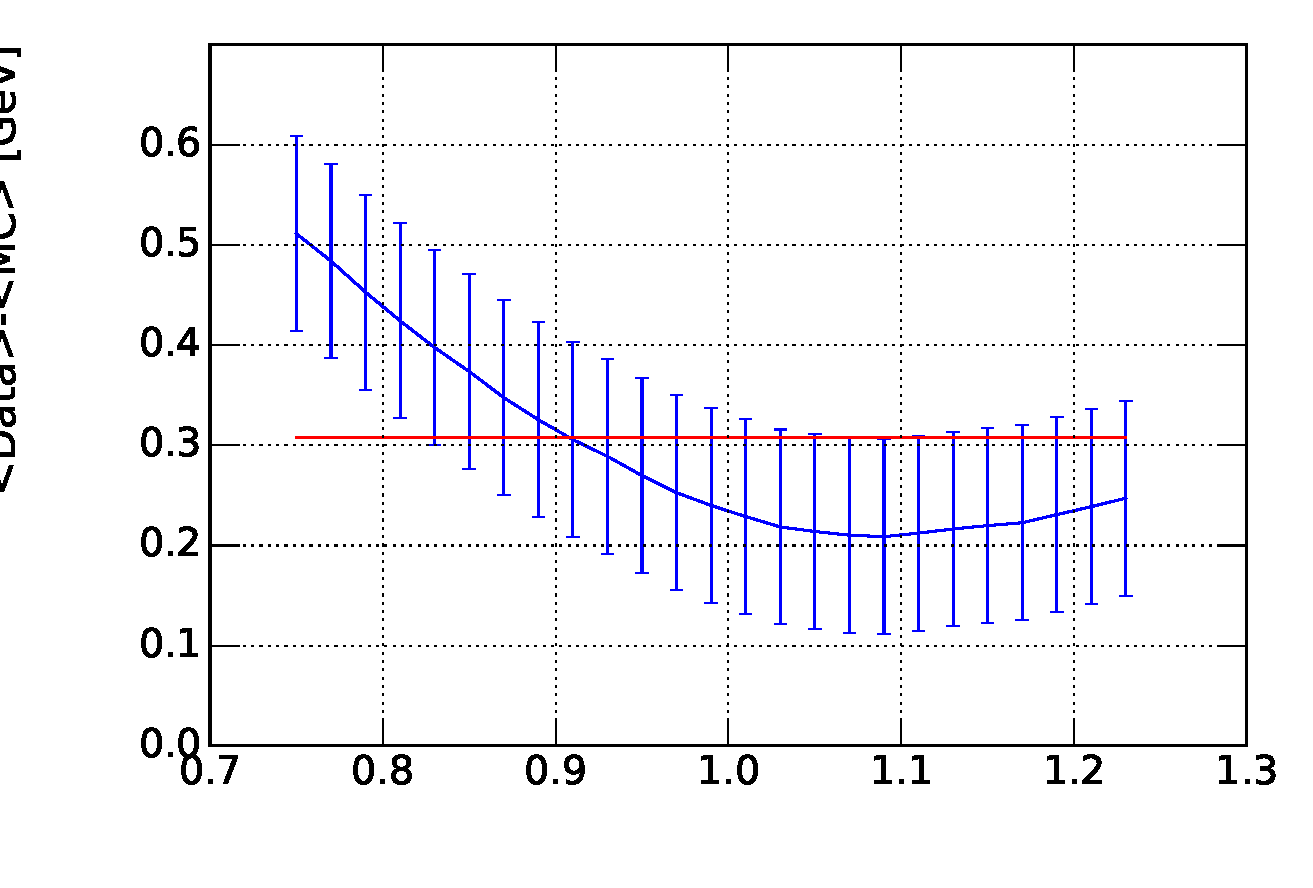
\includegraphics[width=1.\linewidth]{HadronRecoil/MeanCombined.pdf} \\ b)}
\end{minipage}
\caption{Distribution of a difference in a mean transverse mass $<\mtw>$ between the data and simulation as a function of the hadronic recoil correction factor $HR_{SF}$ a) for a different W boson decay channels and b) for combined $W \to l \nu$ selection.}
\label{fig:HRBiasMean}
\end{figure}

One of the possible methods to determine the correction factor is to use a difference in the mean of the transverse mass distributions in data and simulation (Fig.~\ref{fig:HRBiasMean}). Statistical uncertainty on $HR_{SF}$ is considered as a dominant source of uncertainty. Its estimated as a standard error of a mean $\sigma ( <\mtw> ) $, calculated as:
\begin{equation}\label{eq:MeanErr}
\sigma \Big( <\mtw> \Big) = \frac{\sigma( \mtw )}{\sqrt N},
\end{equation}
where $\sigma(\mtw)$ is a standard deviation of $\mtw$ distribution and $N$ is a total number of events. The minimum difference is reached at $HR_{SF}=1.1\pm0.2$. Due to the large statistical uncertainty of this method, it is used as a cross-check for other methods of hadronic recoil bias determination.

\begin{figure}[!tbp]
\begin{minipage}[h]{0.49\linewidth}
\center{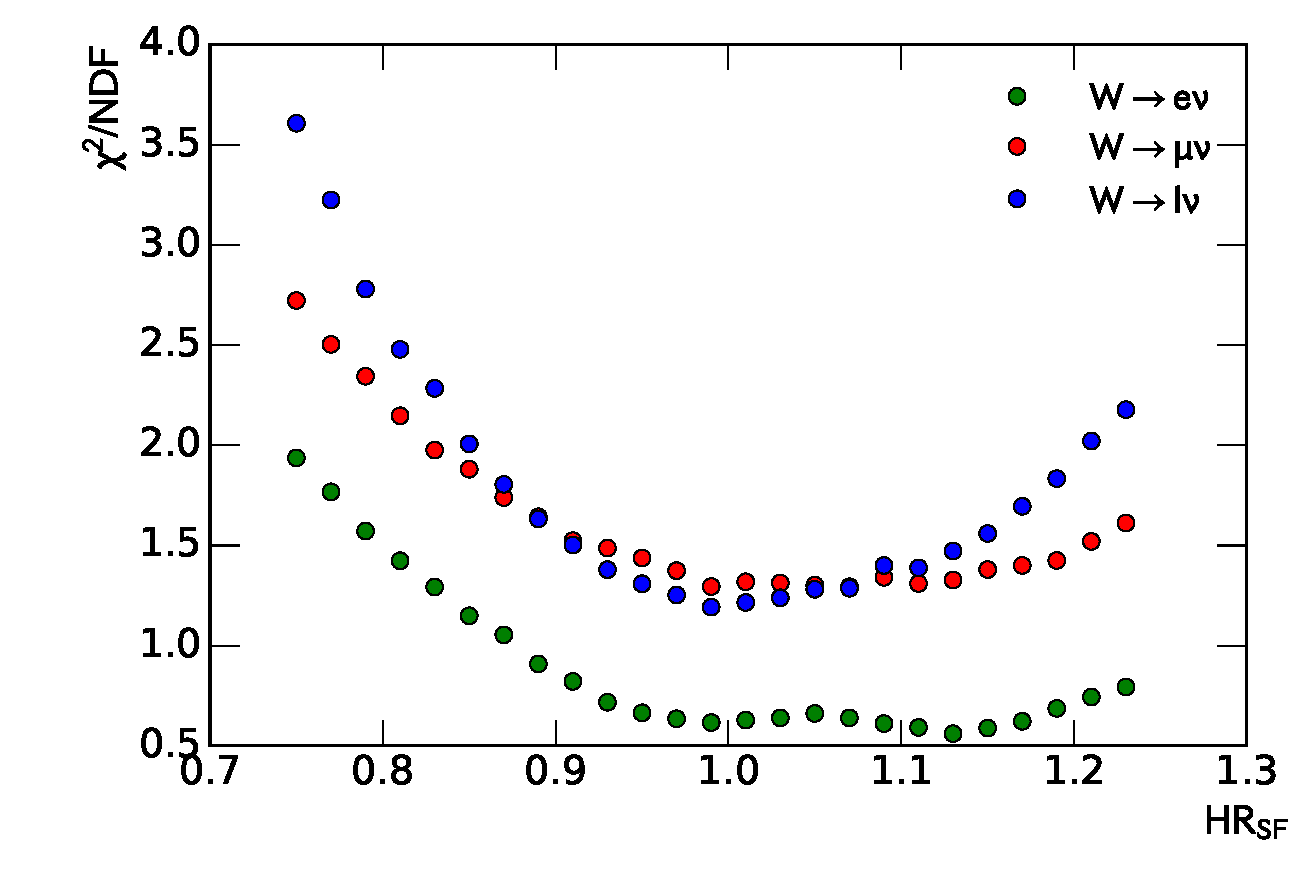
\includegraphics[width=1.\linewidth]{HadronRecoil/chi2AllChannelsMtw.pdf} \\ a)}
\end{minipage}
\hfill
\begin{minipage}[h]{0.49\linewidth}
\center{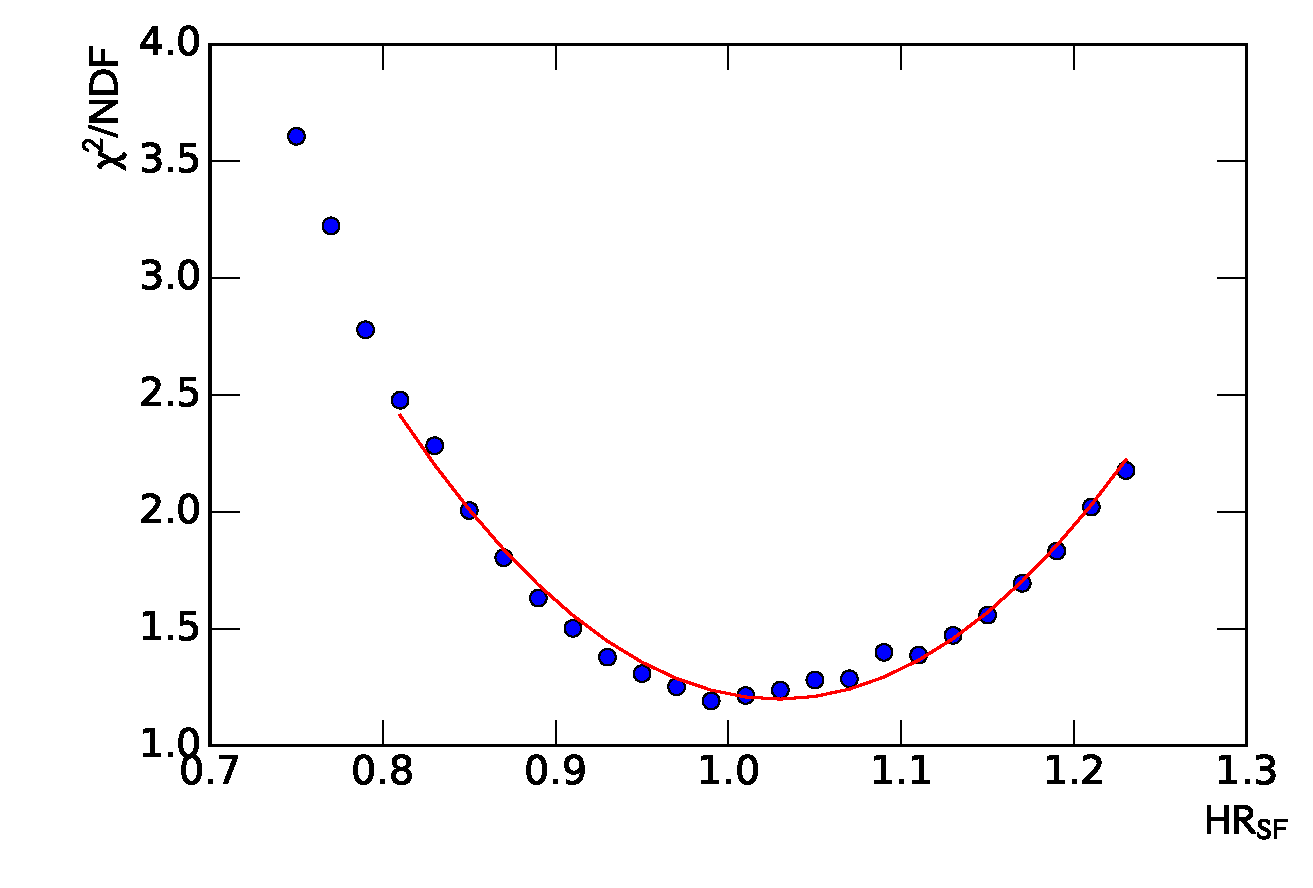
\includegraphics[width=1.\linewidth]{HadronRecoil/chi2TotalMtw.pdf} \\ b)}
\end{minipage}
\caption{Distribution of \chiD-test results for and simulation  for $<\mtw>$ distribution as a function of hadronic recoil correction factor $HR_{SF}$ a) for different W boson channels. 
b) for combined $W \to l \nu$ selection and the \chiD fit results.}
\label{mtWChi2}
\end{figure}

\begin{figure}[!tbp]
\centering
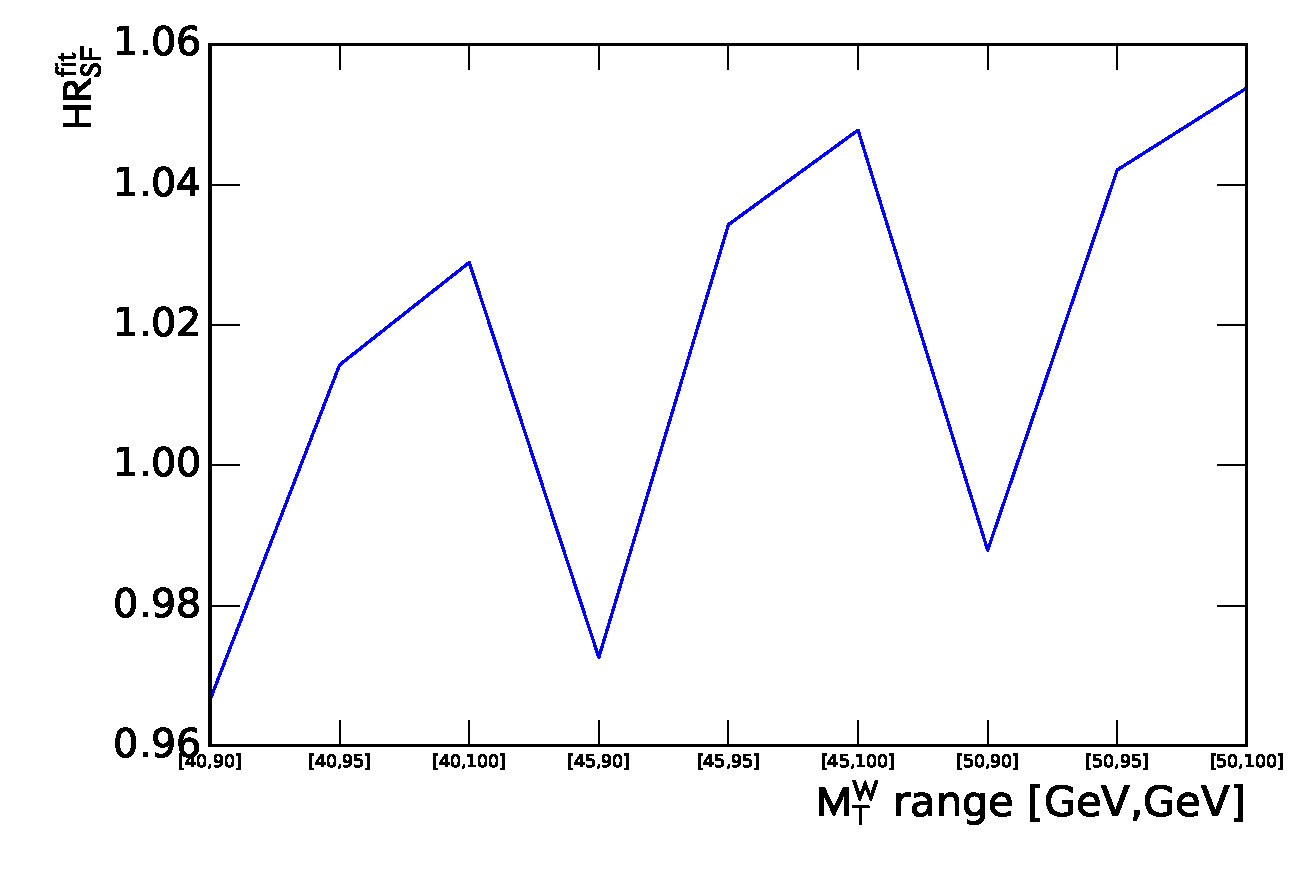
\includegraphics[width=0.5\textwidth]{HadronRecoil/RangeEffect.pdf}
\caption{Hadronic recoil scale correction factors as a function of \mtw fit range. }
\label{ScaleMtWRange}
\end{figure}

Distribution of \chiD-test values for different values of $HR_{SF}$ for W selection is shown in Fig.~\ref{mtWChi2} a). Because of a possible mismodelling of the tail of the \mtw distribution, events with \mtw > 100 GeV are not included in a \chiD-test. There is a small peak visible in the \chiD distribution for \wenu events, that is assumed to come from the missing multijet background contribution. Hadronic recoil bias parameters determined through the fit of \chiD-test distribution in combined $W\to l\nu$ analysis using Eq.~\ref{eq:chiD}. The resulting correction factor is $HR_{SF}=1.02$, with the statistical uncertainty of 0.06. 

The range of the \mtw distribution used in the \chiD-test introduces an additional source of systematic uncertainty. This uncertainty is estimated by repeating the \chiD-test and \chiD fit procedure for  different \mtw ranges, as shown in Fig.~\ref{ScaleMtWRange}. The resulting hadronic recoil correction factor is $HR_{SF}=1.02\pm0.06(stat.)\pm0.03(syst.)=1.02\pm0.07$. 


\subsection{Bias determination from the \upar distribution}




\begin{figure}[!tbp]
\minipage{0.32\textwidth}
  \center{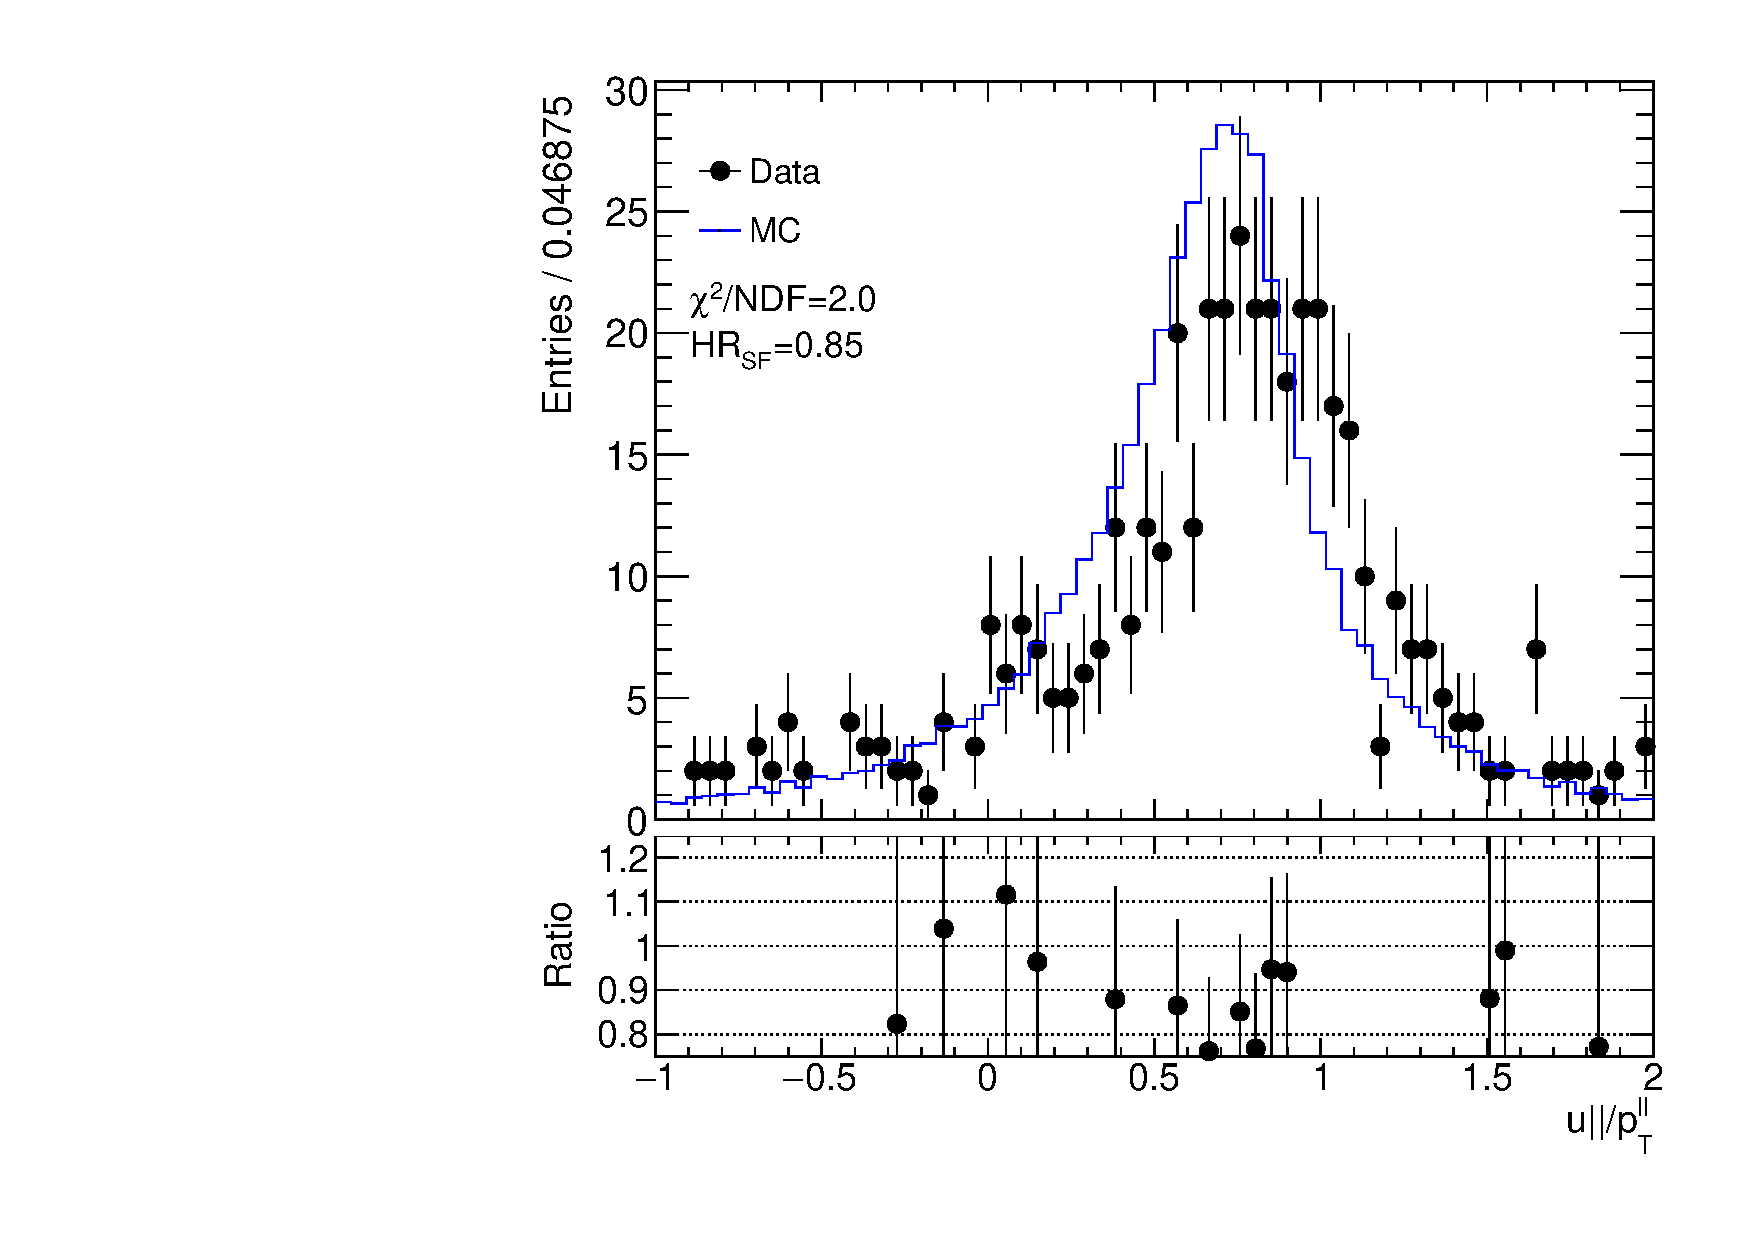
\includegraphics[width=\linewidth]{HadronRecoil/UParEScale5.pdf} a)}
\endminipage\hfill
\minipage{0.32\textwidth}
   \center{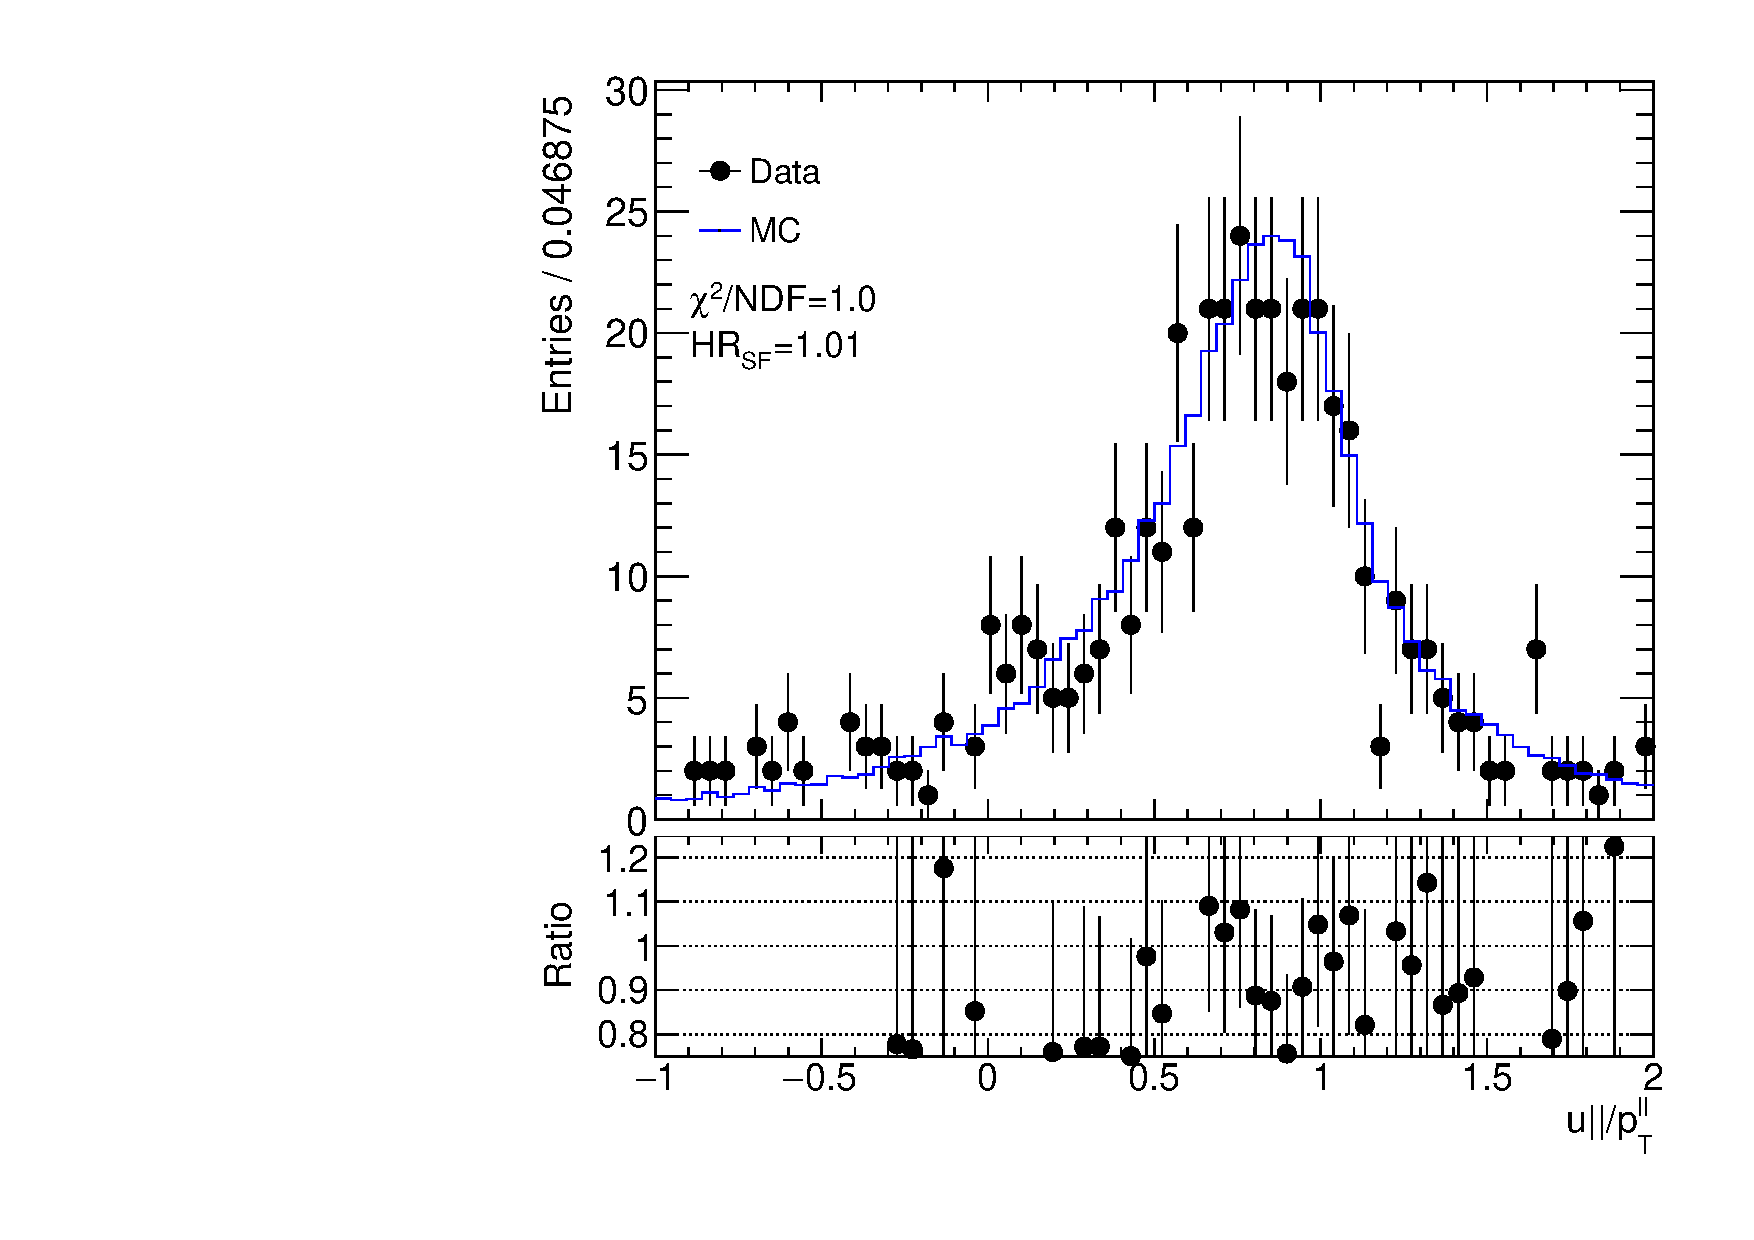
\includegraphics[width=\linewidth]{HadronRecoil/UParEScale13.pdf} b)}
\endminipage\hfill
\minipage{0.32\textwidth}%
   \center{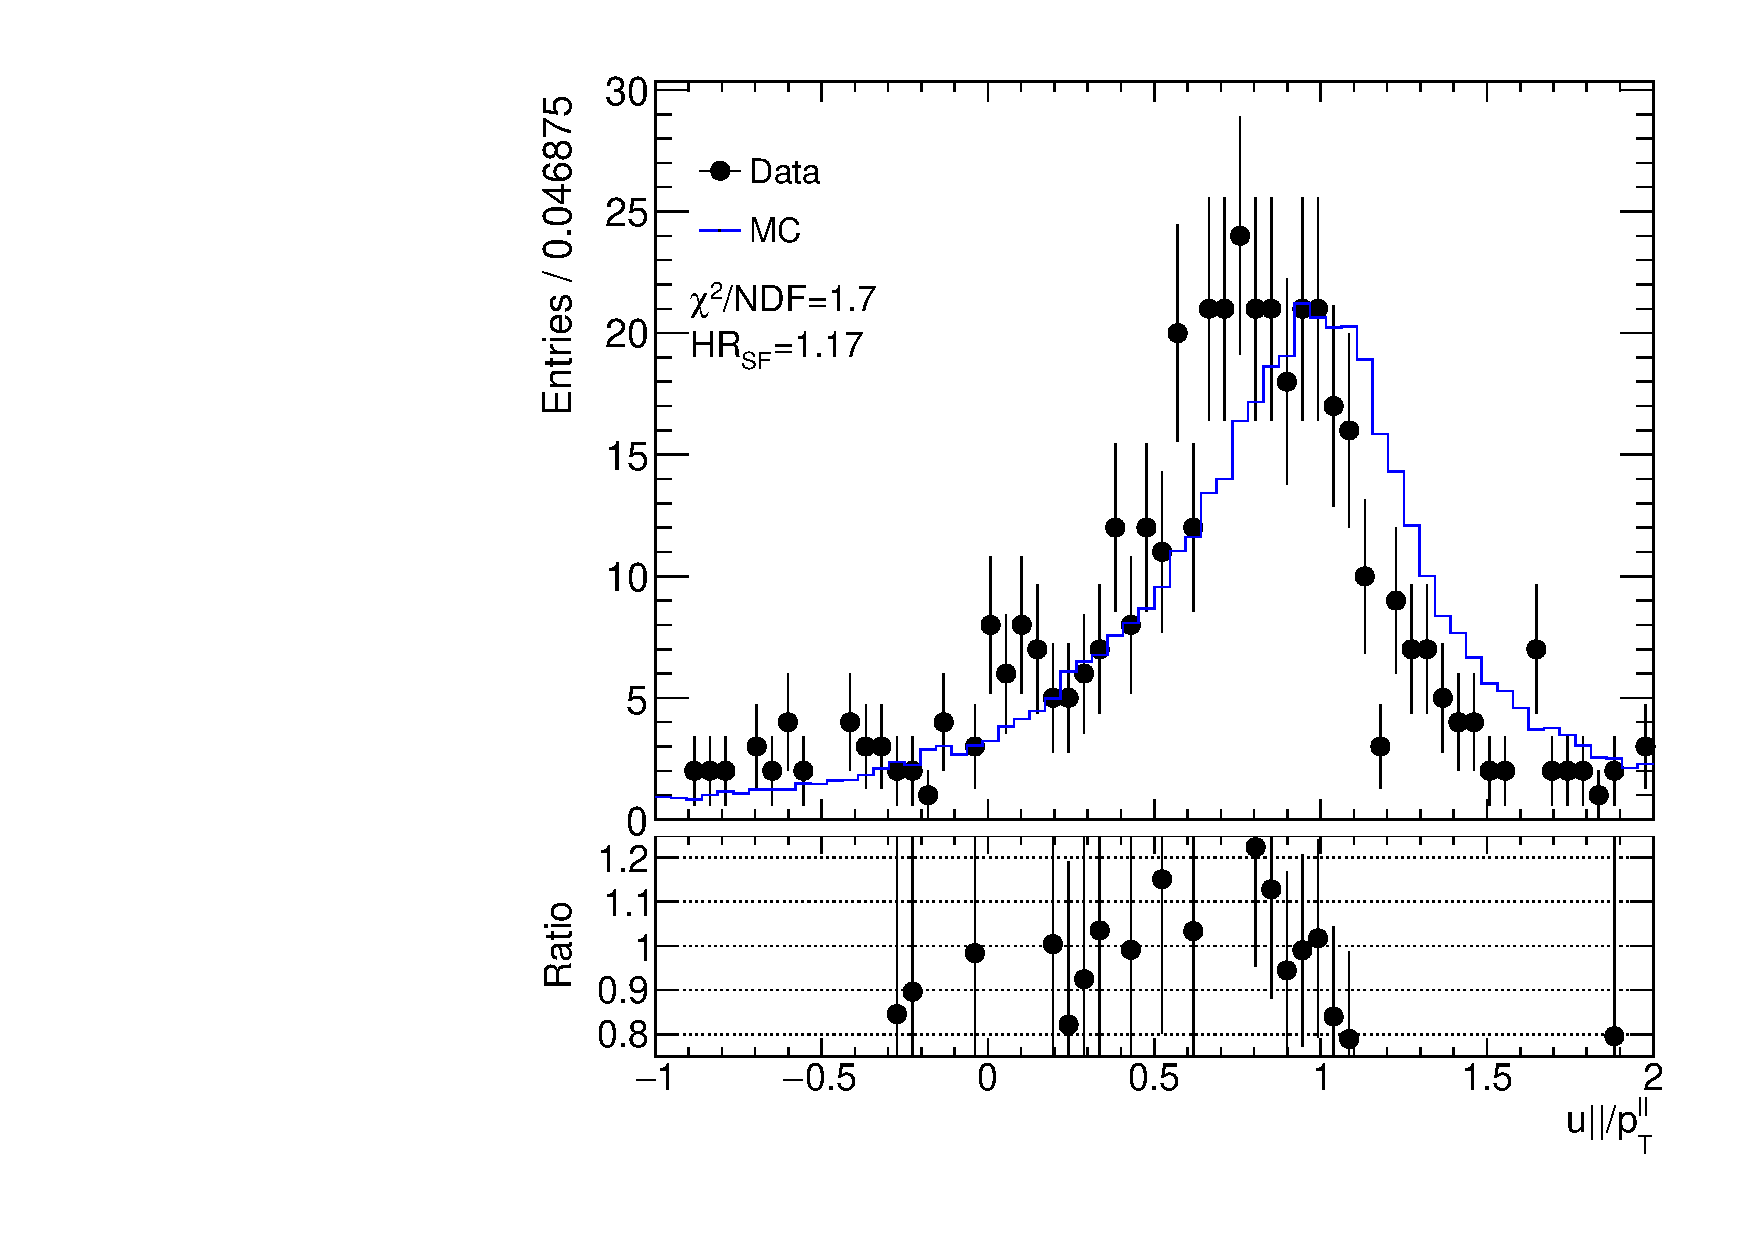
\includegraphics[width=\linewidth]{HadronRecoil/UParEScale21.pdf} c)}
\endminipage
\caption{Hadronic recoil component \upar divided by the transverse momentum of the Z-boson for $Z\to ee$ event selection for different hadronic recoil correction factors: a) $HR_{SF}$=0.75, b) $HR_{SF}$= 1.1 and c) $HR_{SF}$=1.23.}
\label{HadrRecoil:ZScan}
\end{figure}

\begin{figure}[!tbp]
\begin{minipage}[h]{0.49\linewidth}
\center{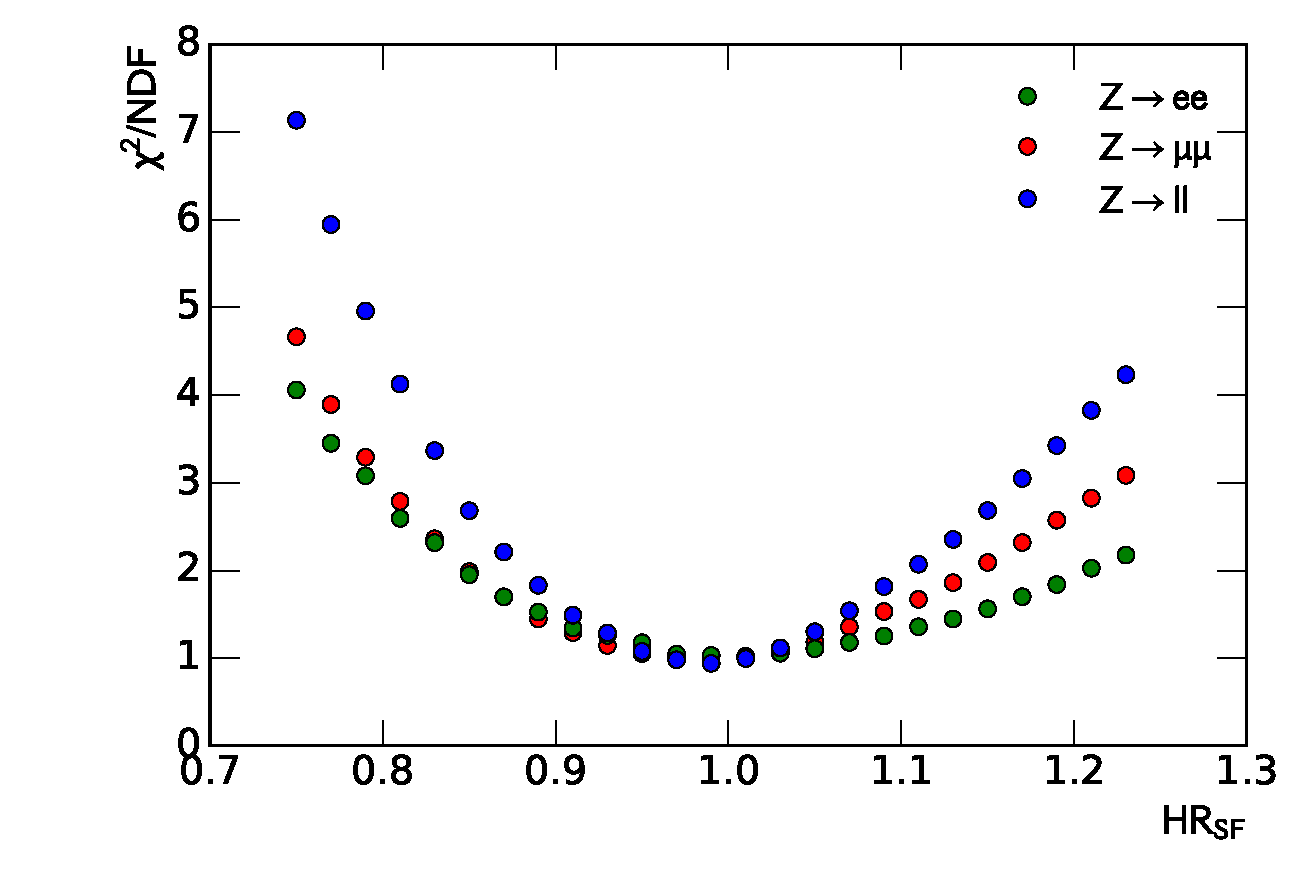
\includegraphics[width=1.\linewidth]{HadronRecoil/chi2Upar.pdf} \\ a)}
\end{minipage}
\hfill
\begin{minipage}[h]{0.49\linewidth}
\center{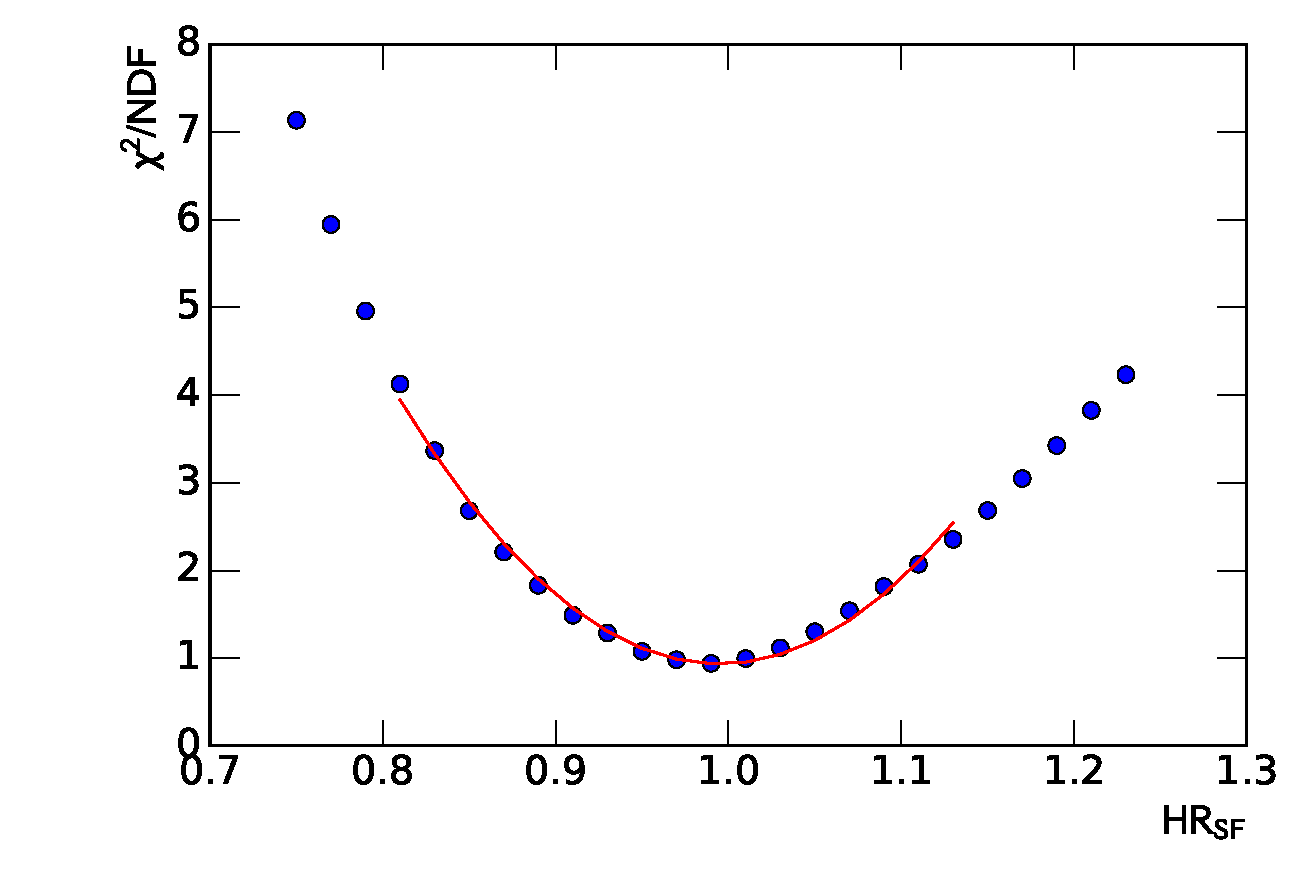
\includegraphics[width=1.\linewidth]{HadronRecoil/chi2UparTot.pdf} \\ b)}
\end{minipage}
\caption{Distribution of \chiD-test values for  data and simulation for $\upar/P_T^{bos}$ distribution as a function of hadronic recoil scale correction factors $HR_{SF}$ for a) different Z boson channels. 
b) for combined $Z \to ll$ selection with the \chiD fit results.}
\label{uPAr}
\end{figure}  
 
The correction factors can be determined from the Z sample using the $\upar/P_T^{Z}$ distribution, as shown in Fig.~\ref{HadrRecoil:ZScan}. Results of the \chiD-test for different values of $HR_{SF}$ for data and simulation for $Z\to ll$ selection are shown in Fig.~\ref{uPAr}. A \chiD fit of the \chiD-test values distribution for combined channel  gives the most precise estimation of the hadronic recoil bias $HR_{SF} = 1.00 \pm 0.01$. 



  
\subsection{Systematic uncertainty estimation}

Summary of a hadronic recoil correction factors is shown in Tab.~\ref{tab:SFHadronRecoil}. The results are consistent with each other within the uncertainty. In the dinal step, it was decided to choose $HR_{SF}$ determined  with the smallest uncertainty (from $Z\to ll$ analysis). Scale factors extracted using other methods are used as a cross-check.


\begin{table}[!tbp]
\caption{Hadronic recoil bias determination results and errors for different methods.}
\label{tab:SFHadronRecoil}
\begin{center}
\begin{tabular}{| l | c | c |}
\hline
Method & SF & error \\
\hline
\hline
Mean $M_T^{W}$ & 1.10 & 0.2\\
$M_T^{W}$ \chiD & 1.01 & 0.07 \\
\upar \chiD & 1.00 & 0.014 \\
\hline
\end{tabular}
\end{center}
\end{table}


Effect of the hadronic recoil bias correction for different bias correction factors are presented in Fig.~\ref{ris:Cw}. Systematic error, coming from the bias correction, is estimated using Offset method (see Chap.~\ref{chap:Unc}). 

\begin{figure}[!tbp]
\begin{minipage}[h]{0.49\linewidth}
\center{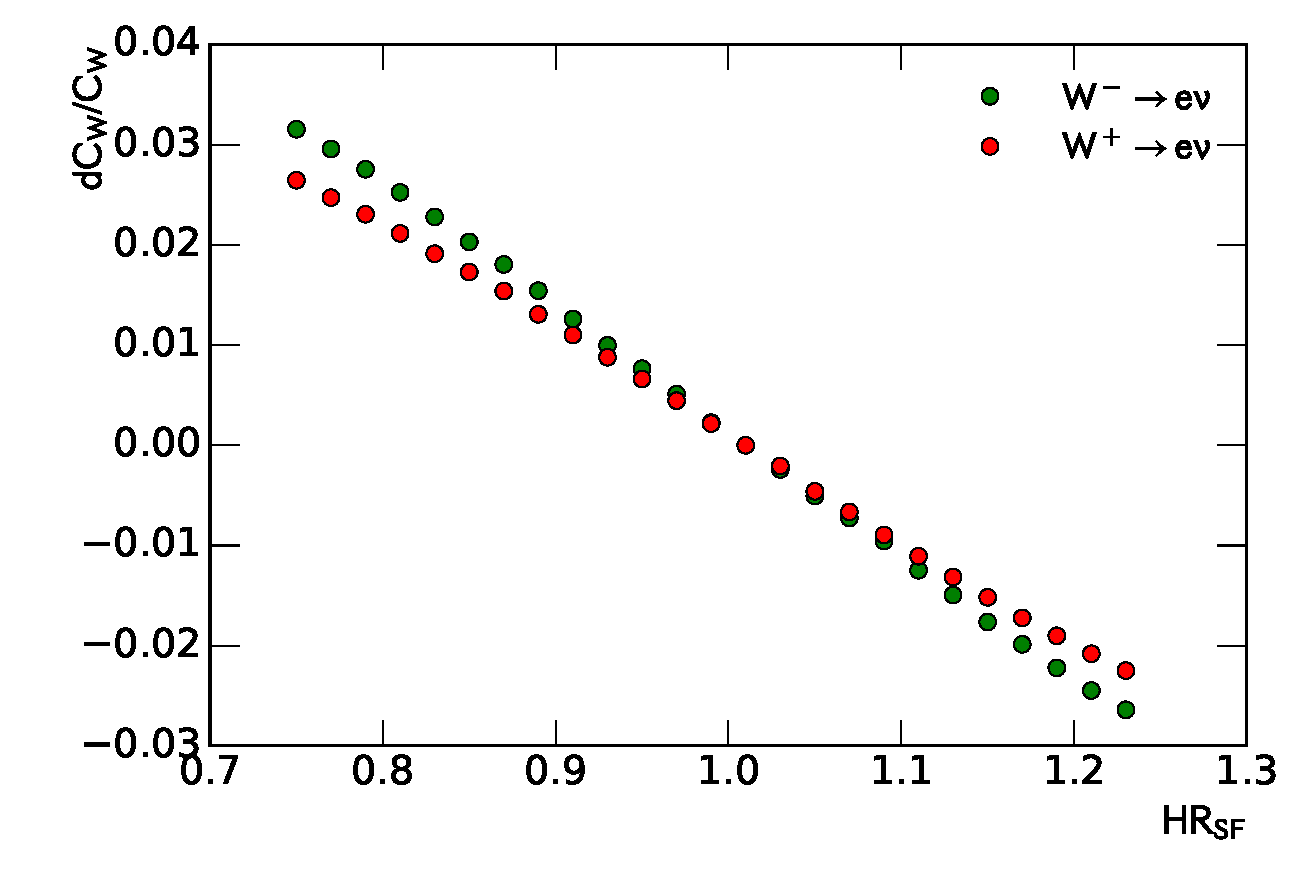
\includegraphics[width=1.\linewidth]{HadronRecoil/CWElectron.pdf} \\ a)}
\end{minipage}
\hfill
\begin{minipage}[h]{0.49\linewidth}
\center{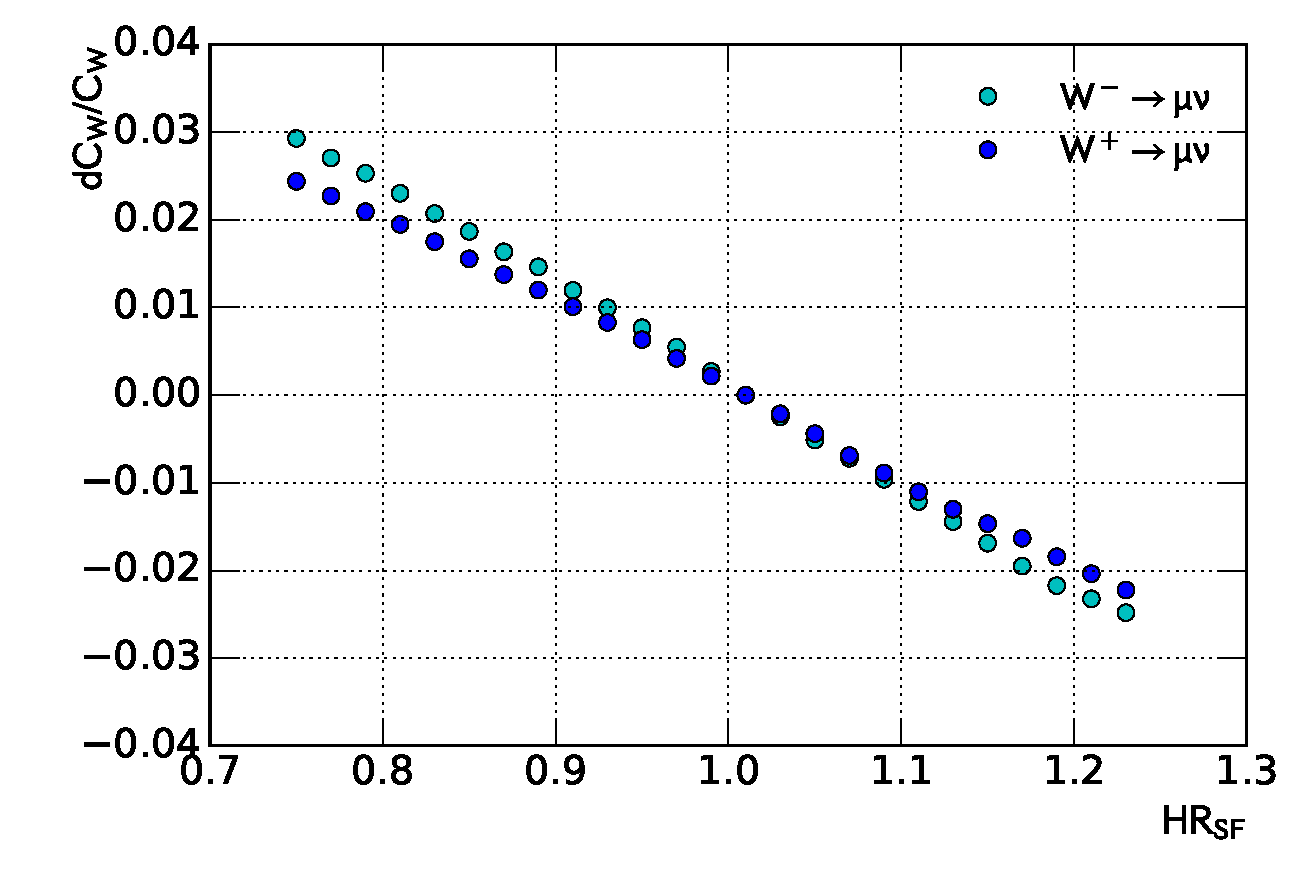
\includegraphics[width=1.\linewidth]{HadronRecoil/CWMuon.pdf} \\ b)}
\end{minipage}
\caption{Shift in the \cw for a different hadronic recoil scale correction factors for a) \wenu b) \wmunu event selection.}
\label{ris:Cw}
\end{figure}


\section{Summary of hadronic recoil calibration}\label{sec:HRSum}
Using the standard \etmiss reconstruction algorithm the data is not described properly by the simulation, therefore  it is decided to use a dedicated hadronic recoil algorithm for \etmiss reconstruction. The methodology of hadronic recoil calibration is developed for the $\sqrt{s}$ = 2.76 TeV data.

The hadronic recoil calibration procedure consists of parts: the correction of resolution effects and the bias correction. 
The hadronic recoil resolution has been corrected using the following methods:
\begin{itemize}
\item Event activity correction through the reweighting of \sumet distribution. Different methods of the data/MC ratio parameterization have been developed and showed a consistent result. However, this method gives a nonphysical difference between electron and muon channels, that cannot be accounted for the data uncertainty, so it was decided to drop this method;
\item Smearing correction of the hadronic recoil. This method uses the Z sample to determine the difference in resolutions of the hadronic recoil components. The overall effect of these corrections was estimated by repeating the smearing 25 times and consistent between electron and muon channels.
\end{itemize}
The bias of hadronic recoil  is estimated using W and Z-boson candidate with the following three methods:
\begin{itemize}
\item Comparison of the mean of the \mtw distributions between data and simulation. This method gives the biggest uncertainty and is used as a cross-check for other results;
\item From the \chiD fit of the \chiD-test results for \mtw distribution for different values of hadronic recoil corrections. Error on this method is dominated by the statistics;
\item From the \chiD fit of the \chiD-test results for $\upar/P_T^{Z}$ distribution for different values of hadronic recoil corrections. Despite the limited statistics of the Z-boson sample, this method gives the biggest sensitivity to the hadronic recoil scale choice. It is therefore decided to use this method as a baseline for the hadronic recoil bias.
\end{itemize}

The corresponding systematic uncertainties for the hadronic recoil calibration are summarized in Tab.~\ref{tab:SFHadronRecoilBias}. The overall uncertainty on \etmiss is around 0.3 \% for  W-boson decay channels.

\begin{table}[!tb]
\caption{Systematic uncertainties from the hadronic recoil calibration for different W boson decay channels.}
\label{tab:SFHadronRecoilBias}
\begin{center}
\begin{tabular}{| l || c | c | c | c |}
\hline
Systematic source & $W^{+} \to e^{+}\nu$ & $W^{-} \to e^{-}\nu$  & $W^{+} \to \mu^{+}\nu$ & $W^{-} \to \mu^{-}\nu$ \\
\hline
\hline
Hadronic recoil resolution & -0.2\% & -0.11\% & -0.16\% & -0.12\% \\
Hadronic recoil scale &  0.21\% & 0.20\% & 0.23\% & 0.24\% \\
\hline
\end{tabular}
\end{center}
\end{table}
